%!TEX root = these.tex

\chapter[Taxinomie des environnements de sélection]{Taxinomie des environnements de sélection de cibles en mouvement}
\minitoc
\label{chap3}
\cleardoublepage

% TODO: Schémas ou tableau pour illustrer le sens de certains critères, genre ciné-discret vs. ciné-continu, etc.
% TODO: Générer des trajectoires avec le modèle VFA à mémoire, pour prouver que ça marche.
% TODO: Idem newtonien ?

\section{Introduction}
	Au cours du premier chapitre de ce manuscrit, nous avons identifié et décrit les besoins de différents domaines d'expertise liés à l'activité de sélection de cibles mobiles. Nous nous sommes en particulier attachés à caractériser la nature des cibles mobiles que l'on rencontre dans ces applications, afin de permettre au lecteur d'apprécier d'une part l'ensemble des difficultés inhérentes aux tâches de sélection dans ces applications, et d'autre part la nécessité d'une assistance à la sélection.
	
	Si nous avons jusqu'ici énuméré et caractérisé ces types de cibles, avec une attention toute particulière à leur contexte applicatif, nous n'avons pas procédé à une classification systématique des cibles selon la nature de leur mouvement, définie selon des critères objectifs et des mesures quantitatives. Or, il nous apparaît que pour réellement comprendre les enjeux et défis liés à la sélection de cibles mobiles, une telle classification est nécessaire.
	
	L'objectif de ce chapitre est donc d'établir une taxinomie des cibles mobiles selon des critères objectifs et, dans la mesure du possible, de permettre une quantification des valeurs auxquelles ils se rapportent. Nous commençons par exposer nos réflexions sur les critères à retenir pour établir cette taxinomie, puis nous confrontons les cibles et leurs environnements à ces critères. Nous présentons ensuite un modèle que nous avons développé pour décrire et générer du mouvement pseudo-aléatoire, régi par des paramètres finement contrôlés. Nous nous appuyons sur ce modèle pour compléter notre taxinomie par des mesures quantitatives et objectives de différents cas applicatifs mobilisant une activité de sélection de cible mobile.	
	
	\section{Critères de discrimination et nature du mouvement}
	Bien qu'une \og simple \fg{} taxinomie des cibles mobiles en fonction de la nature de leur mouvement ait beaucoup d'intérêt, elle ne saurait fournir suffisamment d'informations pour guider la conception de techniques de sélection sans tenir compte de l'\emph{environnement} de sélection. En effet, la cible la plus petite, la plus rapide et la plus imprévisible imaginable est triviale à sélectionner s'il s'agit du seul objet d'intérêt dans l'environnement : il n'y a qu'une sélection possible, donc la technique de sélection optimale --- ou du moins suffisante --- consiste à permettre la sélection de la cible par la simple pression d'un bouton, ou activation d'un quelconque périphérique de saisie.
	
	Dans un tel cas, du point de vue de la théorie de l'information de Shannon~\cite{shannon2001mathematical}, un seul bit d'information est à transmettre de l'utilisateur au système, correspondant à la réponse à la question suivante : \og la cible doit-elle être sélectionnée ? \fg{}. Si la réponse est négative, l'utilisateur ne fait rien et le système non plus ; si elle est positive, une seule action est nécessaire de la part de l'utilisateur, et le système, qui connaît la position de la cible, n'a qu'à la sélectionner sans requérir de précision de la part de l'utilisateur.
	
	Même dans un cas où il y aurait plusieurs objets de ce type, mais en petit nombre, la sélection demeurerait relativement aisée avec une technique telle que le \emph{Bubble Cursor}, analysée au cours du deuxième chapitre. En effet, cette technique illustrée par la figure~\ref{fig:bubble} partage l'espace en plusieurs cellules, selon un diagramme de Voronoï (voir la figure~\ref{fig:voronoi}). De fait, avec par exemple quatre cibles (même très petites, rapides et imprévisibles) l'espace virtuel serait partagé en quatre parties qui, la plupart du temps, seraient très grandes. La loi de Fitts ne s'appliquerait pas directement, car ces zones de sélection seraient mobiles, mais l'on voit bien que la sélection ne serait pas très difficile.
	
	À l'inverse, avec des cibles aussi petites, rapides et imprévisibles, mais extrêmement nombreuses, l'on comprend aisément que l'intérêt du \emph{Bubble Cursor} serait très fortement diminué car les cellules de Voronoï de chaque cible deviendraient fort petites, et pas nécessairement significativement plus grandes que les cibles elles-mêmes.
	
	Il apparaît donc clairement que la difficulté d'une tâche de sélection ne peut être évaluée qu'en tenant compte de l'environnement dans lequel l'objet ciblé est sélectionné. De fait, les besoins et contraintes devant orienter la conception d'une technique d'assistance doivent également en tenir compte. Aussi notre taxinomie tiendra-t-elle compte de l'environnement global, et non seulement de la cible à sélectionner et de la nature de ses mouvements.


	L'établissement de notre taxinomie passe par le choix des critères qui nous permettront d'établir des distinctions entre les types de mouvements des cibles et les environnements de sélection. Dans les sous-sections suivantes, nous allons détailler les critères que nous avons retenus.
	
	\FloatBarrier \subsection{Dimensionnalité}
	Les cibles et leurs environnements se caractérisent notamment par leur nombre de dimensions spatiales. En soi, ce nombre peut varier de un à trois, mais les applications à une seule dimension sont trop rares et trop spécifiques pour entrer dans le cadre de nos travaux. Demeurent donc les objets évoluant dans des espaces 2D/3D. En pratique, la dimensionnalité de l'environnement \og écologique \fg{} des cibles ne correspond pas forcément à la dimensionnalité du dispositif d'affichage ou d'interaction. Les avions, par exemple, évoluent dans un espace tridimensionnel, mais sont généralement affichés sur un plan en 2D sur lequel ils sont projetés ; les périphériques de saisie permettant de les sélectionner sont aussi, généralement, limités à deux degrés de liberté.
	
	\FloatBarrier \subsubsection{Environnements 2D}
	Le contrôle de la circulation routière et des espaces maritimes sont des exemples d'environnements bidimensionnels, si l'on néglige les variations d'altitude sur les routes, les ponts, etc. La surveillance des signaux électromagnétiques entre également dans cette catégorie. Les jeux vidéos tels qu'\emph{Agar.io} (voir figure~\ref{fig:agario}) peuvent aussi présenter des environnements de ce type.
	
	\FloatBarrier \subsubsection{Environnements 3D projetés sur un plan}
	De nombreux types d'objets évoluent dans des environnements 3D mais sont couramment visualisés et sélectionnés à l'aide de systèmes 2D --- par choix, car il est généralement possible d'utiliser des systèmes 3D, et pour certaines applications, c'est occasionnellement le cas. Notons ici les applications pouvant entrer dans la catégorie \og 3D projetée en 2D \fg{}, qu'elles puissent également intégrer la catégorie 3D ou non. Citons donc les simulations moléculaires, le contrôle de l'espace aérien, extra-atmosphérique, maritime quand les sous-marins sont pris en compte, la vidéo-surveillance quand les environnements présentent de forts écarts d'altitude (comme dans un simple bâtiment à plusieurs étages), les retransmissions d'événements sportifs, et enfin la plupart des jeux vidéo dits \og en 3D \fg{} --- à ne pas confondre avec l'immersion en 3D rendue possible par la \emph{stéréoscopie}.
	
	\FloatBarrier \subsubsection{Environnements 3D}
	Parfois, il est possible d'interagir avec un environnement 3D à l'aide d'un dispositif de visualisation immersif et un périphérique de saisie adapté, ayant généralement au moins trois degrés de liberté. C'est occasionnellement le cas des simulations moléculaires et autres applications scientifiques, de certains jeux vidéo, et potentiellement de toutes les applications mentionnées dans la catégorie \og 3D projetée en 2D \fg{}, même si nous n'avons pas connaissance, par exemple, de tels systèmes actuellement utilisés pour le contrôle de l'espace aérien.

	\FloatBarrier \subsection{Autocorrélation}
	Nous considérons ici qu'un mouvement est autocorrélé si un \emph{changement de direction} opéré à l'instant $t$ dépend du \emph{changement} (éventuellement nul) opéré à l'instant $t-1$. Si, au contraire, un changement peut avoir lieu à l'instant $t$ quelle que fût la situation à l'instant précédent, nous appelons ce mouvement \emph{markovien}~\cite{markov1960theory} en admettant qu'il s'agit d'un abus de langage, puisqu'un processus respectant la propriété de Markov est totalement indépendant de l'état du système à l'instant précédent ; or, ici, le vecteur vitesse d'un objet à l'instant $t$ peut dépendre de son orientation à l'instant $t-1$ même si le changement d'orientation n'en dépend pas.
	
	En effet, si ledit changement se fait selon un angle borné (entre -10\textdegree{} et +10\textdegree{}, par exemple) alors l'orientation du vecteur vitesse à l'instant $t$ dépendra de son orientation à $t-1$, puisqu'elle ne pourra différer de celle-ci que de 10\textdegree{}. Tant que le \emph{changement} de direction à l'instant $t$, lui, est bien indépendant du \emph{changement} à l'instant $t-1$, nous admettons cet abus de langage et parlons de mouvement markovien.
	
	Dans le cas contraire, le mouvement est dit autocorrélé. Par exemple, un véhicule effectuant un virage à un instant $t$ est susceptible de maintenir ce virage --- donc le changement de direction correspondant --- à l'instant $t+1$ : le fait que le changement de direction à un instant influence celui de l'instant suivant constitue ce que nous appelons l'autocorrélation. Par commodité, nous appliquons ces termes aux objets autant qu'à leurs mouvements.

	Parmi les objets autocorrélés figurent tous les véhicules que nous avons évoqués au cours du chapitre~\ref{chap1} : les automobiles, navires, aéronefs, engins spatiaux, etc. Au sens strict, tout objet de masse non nulle et macroscopique devrait être autocorrélé, mais nous pouvons considérer que certains peuvent changer de direction de manière si vive et imprévisible qu'ils sont subjectivement markoviens. En règle générale, nous admettons qu'un projectile est autocorrélé, tout en gardant à l'esprit que dans certains cas il peut avoir un comportement subjectivement markovien.
	
	Le cas des jeux vidéo est délicat en ce qu'il s'agit d'un domaine extrêmement vaste dans lequel il est possible de trouver des cibles de toutes natures. Néanmoins, quand ils sont modélisés de manière (subjectivement) réaliste, les objets qui sont autocorrélés dans le monde réel le sont également dans les environnements virtuels des jeux. Enfin, il est possible de rencontrer dans un jeu vidéo n'importe quel type d'objet, réel ou imaginaire. Ceux de la seconde catégorie peuvent être autocorrélés comme markoviens ; il est impossible d'en dresser un inventaire exhaustif, mais disons simplement qu'ils existent --- comme les disques du jeu \emph{Agar.io}, mentionné dans le premier chapitre, qui sont markoviens.

	\FloatBarrier \subsubsection{Uniformité}
	Le mouvement autocorrélé le plus simple est le mouvement uniforme, c'est-à-dire celui pour lequel le vecteur vitesse ne change jamais. Les objets de mouvement uniforme se déplacent donc en ligne droite. Inversement, un mouvement n'est pas uniforme si, à un instant quelconque, la direction ou la norme du vecteur vitesse de l'objet concerné change. Du fait du focus de ce manuscrit sur les cibles mobiles de sélection difficile, nous n'avons pas réellement abordé d'objets aux mouvements uniformes au cours du premier chapitre. Il va sans dire qu'ils existent pourtant. Remarquons néanmoins que si l'on restreint suffisamment la fenêtre temporelle au travers de laquelle on analyse le mouvement d'un objet, l'on peut généralement aboutir à un mouvement localement uniforme.
	
	C'est notamment le cas de véhicules, et particulièrement de ceux qui couvrent de longues distances. Ainsi, les avions et les navires suivent généralement des géodésiques\footnotemark{}, et même une automobile sur une autoroute tend à suivre une trajectoire rectiligne si l'on n'en observe que quelques centaines de mètres. Même un piéton sur un trottoir ou un athlète sur une piste de course peuvent avoir une trajectoire localement uniforme. Les projectiles ayant des trajectoires balistiques, ils ne sont pas de mouvement uniforme, mais peuvent le paraître si ce mouvement est projeté sur un plan horizontal, masquant les variations d'altitude (quoique des variations de vitesse puissent demeurer perceptibles). %Pour être tout à fait exact, un projectile tournant sur lui-même dans l'air (ou un autre fluide) est soumis à l'effet Magnus~\cite{magnus1853ueber, briggs1959effect} et n'a donc pas une trajectoire balistique ; selon l'axe de sa rotation, il peut donc ne pas avoir un mouvement rectiligne une fois sa trajectoire projetée sur un plan horizontal. C'est par exemple le cas d'un ballon de football suite à une \og frappe enroulée \fg{}.

	
	\footnotetext{Une géodésique est une ligne droite sur une surface de géométrie quelconque. Sur une sphère, une géodésique est un \emph{grand cercle}.}
	
	\FloatBarrier \subsubsection{Périodicité}
	Un mouvement sera dit périodique si les changements de direction sont tels que l'objet effectuera une trajectoire qu'il répétera (éventuellement sur une partie seulement) à intervalles réguliers. Plus formellement, un mouvement est périodique s'il admet une période $T$ telle que :	$\forall t,~Pos_{t}~=~Pos_{t+T}$ où $Pos_{t}$ désigne la position de l'objet à l'instant $t$.
	
	Là encore, du fait du focus de ce manuscrit, les objets de mouvement périodique ont peu été abordés au cours du premier chapitre. On les trouve cependant dans certains jeux vidéo, ainsi que dans des applications astronomiques, les objets célestes étant généralement en orbite autour d'un point de l'espace. Les débris spatiaux sont donc des exemples d'objets de mouvement périodique, même s'ils sont susceptibles d'être examinés sur des échelles temporelles trop courtes pour que cette périodicité soit perceptible. Ce n'est cependant pas nécessairement le cas, par exemple si l'on souhaite étudier ces objets dans leur ensemble et sur un temps relativement long, afin d'examiner les dangers qu'ils représentent. La densité de ces objets rend par ailleurs ce cas particulièrement intéressant ; en ceci, nous pouvons le rapprocher de l'étude des anneaux de certaines planètes\footnotemark{}.
	
	\footnotetext{Le cas de Saturne est d'autant plus intéressant qu'en plus d'être nombreux et très riches, ses anneaux ont été étudiés de très près et longuement par la sonde \emph{Cassini}, de sorte que nous avons des informations détaillées dessus.
	
	\url{https://saturn.jpl.nasa.gov/mission/grand-finale/grand-finale-orbit-guide}}
	
	\paragraph{Pseudo-périodicité.}
	Nous appellerons pseudo-périodique un mouvement caractérisé par une trajectoire répétée à intervalles \emph{irréguliers}. Un tel mouvement ne satisfait pas la condition formalisée ci-dessus, mais admet un ensemble de positions limitées à une trajectoire donnée, et revisitées continuellement dans le même ordre --- simplement, à des vitesses pouvant varier.
	
	Les objets de mouvement pseudo-périodique sont très proches (subjectivement) de ceux de mouvement périodique. Ils sont également assez rares dans les applications impliquant une tâche de sélection de cible mobile. Nous pouvons néanmoins citer les véhicules de course sur circuit. Compte tenu des durées des pseudo-périodes concernées, il est cependant peu probable que la pseudo-périodicité soit perceptible par un utilisateur, à moins bien sûr qu'il ne visionne un enregistrement de la course en accéléré. Une telle activité pourrait avoir de l'intérêt, par exemple pour une écurie de Formule~1 cherchant à analyser une course terminée.
	
	\paragraph{Ellipticité et pseudo-ellipticité.}
	Un mouvement (pseudo-)périodique peut être elliptique, voire circulaire. Nous considérons en pratique que les implications pour la tâche de sélection sont presque identiques.
	
	Nous avons déjà examiné le cas des objets célestes dans la catégorie des objets de mouvement périodique, aussi n'est-il pas utile d'y revenir ici, si ce n'est pour préciser qu'ils appartiennent évidemment à la catégorie des objets de mouvement elliptique lorsqu'ils sont en orbite~\cite{kepler1953epitome}. Rares sont les objets non célestes suivant de telles trajectoires, bien que les voitures de course de type NASCAR ou les chevaux de course s'en approchent.
	
	\subsection{Vitesse}
	La vitesse des cibles est un critère essentiel de notre taxinomie, car cette valeur a une très forte influence sur la difficulté de sélection, comme le montrent notamment les résultats empiriques obtenus par Ortega~\cite{ortega2013hook} (voir section~\ref{sub:hook}), ainsi que les travaux de Jagacinksi \emph{et al.}~\cite{jagacinski1980test} (voir section~\ref{sub:fittsMobile}) et ceux d'Al Harji \emph{et al.}~\cite{hajri2011moving} (section~\ref{sub:fittsMobile}). Plus une cible est rapide, plus elle est difficile à sélectionner. Nos propres mesures, sur lesquelles nous reviendrons en détail plus loin, le confirment.
	
	La vitesse \emph{absolue} de la cible n'est pas très importante, seule sa vitesse \emph{relative} (observée à l'écran) compte. Par exemple, la Terre effectue sa rotation autour du Soleil à près de 30~km/s, soit 108~000~km/h. Cette vitesse réelle a pourtant peu de chances d'être un problème dans une application réelle, car une telle application présenterait probablement la Terre à une échelle permettant d'observer son orbite. Or, la Terre mettant environ 365 jours à compléter son orbite, sa vitesse relative serait très faible, donc peu gênante dans une tâche de sélection. À l'inverse, une balle de tennis est comparativement lente ($\approx$~200~km/h), mais étant observée à l'échelle d'un court de tennis (environ 24~m) sa vitesse relative est considérable. De même, un objet dans un jeu vidéo peut se déplacer très lentement, à quelques cm/s seulement ; mais si ce mouvement est observé à l'échelle 1, alors l'objet traversera un écran standard très rapidement.
	
	Or, notre taxinomie vise à classifier les cibles et leurs environnements selon les difficultés de sélection qu'ils présentent et non selon leurs caractéristiques absolues ; de fait, nous nous intéressons aux vitesses relatives des objets examinés. Ce choix est lourd de conséquences car la vitesse relative d'un objet d'une vitesse réelle donnée dépend des conditions dans lesquelles il est affiché, en particulier de l'échelle relative à la taille du dispositif d'affichage, et de ladite taille. Elle dépend également, pour tout ce qui n'est pas joué à vitesse réelle, de la vitesse choisie pour l'animation ou la simulation.
	
	La taxinomie que nous proposons implique de faire des choix. La vitesse des objets est un critère de discrimination essentiel, qui impose de discrétiser un espace continu. Dans un souci de simplicité, nous avons choisi de le réduire à deux catégories : les objets rapides et les objets lents. Ce choix est quelque peu arbitraire et subjectif, mais nécessaire, et nous semble d'autant plus justifié que c'est justement l'impression subjective des utilisateurs face à un certain type de mouvement qui nous intéresse, car nous faisons l'hypothèse (sur laquelle nous reviendrons) que cette impression subjective est corrélée aux performances de sélection.
	
	\FloatBarrier \subsubsection{Variabilité de la vitesse}
	Il serait pratique de pouvoir résumer la vitesse à une variable scalaire, mais ce n'est malheureusement pas toujours possible. En effet, dans les applications identifiées le long du chapitre~\ref{chap1}, la vitesse des objets est généralement variable. L'on ne saurait donc la résumer par un simple nombre. Dans l'idéal, il serait bon de connaître toutes les vitesses atteintes par les objets de la scène, avec leurs fréquences d'occurrence ; cela nous permettrait d'en dresser un histogramme. Connaissant toutes ces valeurs, l'on pourrait les représenter de façon plus concise par une moyenne et un écart-type ; il serait sans doute opportun d'ajouter à cette représentation la vitesse maximale possible, afin de pouvoir caractériser le cas (potentiellement) le plus difficile. Pour certaines applications, il sera difficile voire impossible d'avoir des informations aussi précises. Dans ce cas, nous devrons nous contenter d'une estimation aussi précise que possible des valeurs sus-citées, par exemple d'une vitesse \og typique \fg{} et d'une vitesse maximale.
		
	\FloatBarrier \subsubsection{Objets lents, objets rapides}
	Le mode de visualisation détermine souvent la vitesse apparente des objets. À grande échelle, les véchicules paraissent lents. En règle générale, les piétons observés dans des enregistrements de mouvements de foule sont assez lents, exception faite des émeutes, où les mouvements se font plus vifs. À petite échelle, tout type de véhicule peut paraître rapide. La lenteur d'une cible mobile rend sa sélection plus aisée, mais des objets lents peuvent néanmoins être petits, distants, présents dans des environnements très denses, (partiellement) occultés, et caractérisés par des mouvements imprévisibles. Il serait donc imprudent de considérer qu'ils sont \og faciles \fg{} à sélectionner sur la seule base de leur lenteur.
	
	Dans la grande majorité des cas, les particules des simulations moléculaires sont (très) rapides à l'écran. Les athlètes peuvent également être assez rapides (les skieurs ou patineurs de vitesse, par exemple) mais c'est encore plus vrai des projectiles qu'ils utilisent. Enfin, les jeux vidéo regorgent d'objets de vitesses extrêmement variées, et il n'y a pas de borne maximale pratique à la vitesse des objets vidéoludiques.
	
	\FloatBarrier \subsubsection{Accélération}
	Au-delà des valeurs moyennes/typiques ou maximales de la vitesse, il peut être judicieux d'examiner dans quelle mesure la vitesse peut varier en un court laps de temps, c'est-à-dire de détailler la façon dont les objets sont susceptibles d'accélérer. En effet, un objet se déplaçant relativement lentement peut paraître aisé à sélectionner, mais s'avérer fort difficile s'il accélère brutalement, surtout si cette accélération a lieu précisément au moment où l'utilisateur effectue son mouvement de sélection.
	
	Là encore, l'idéal serait d'avoir un histogramme, ainsi qu'une moyenne, un écart-type et une valeur maximale. L'on devra plus souvent se contenter d'une valeur typique et d'une valeur maximale estimées. Ce sera généralement suffisant pour répondre à la question primordiale concernant l'accélération : \og la cible est-elle susceptible d'accélérer brusquement ? \fg{}. Les objets accélèrent généralement d'autant plus facilement qu'ils sont légers, et que les atomes peuvent le faire brusquement, y compris dans les simulations de dynamique moléculaire.

	Les objets de vitesse \emph{strictement} constante sont rares, mais pas inexistants. La table~\ref{tab:dotamoves}, par exemple, fournit les vitesses des personnages les plus vifs d'un jeu vidéo, et ces vitesses sont constantes (sauf effets magiques ou autres). Certains des objets de mouvement circulaire ont également une vitesse constante. Cependant, si l'on assouplit quelque peu notre critère pour inclure, d'une part, les objets de vitesse \emph{approximativement} constante et, d'autre part, les objets de vitesse constante sur une partie (significative) de leur trajectoire, alors nous pouvons en ajouter un nombre important : de nombreux véhicules, quand une vitesse de croisière est maintenue pendant un temps assez long, ou les objets célestes, pour peu que l'excentricité de leur orbite ne soit pas trop élevée --- car de celle-ci dépendent les variations de vitesse. Cela permet de considérer la Terre, dans son orbite autour du Soleil, comme un objet de vitesse constante. Ajoutons les piétons en marche, ou les athlètes pendant une course d'endurance.
	
	Comme la vitesse, l'accélération est une quantité réelle. De fait, son utilisation comme critère de discrimination implique de la discrétiser. Distinguons simplement les objets dont l'accélération est négligeable de ceux dont elle est clairement perceptible ou particulièrement élevée. Nous définissons ici l'accélération comme la dérivée de la \emph{vitesse} (la valeur scalaire représentant la norme de la vélocité) et non de la \emph{vélocité} (qui est une valeur vectorielle). Nous partons donc du principe qu'un objet changeant brusquement de direction tout en maintenant une vitesse constante a une \og accélération \fg{} nulle, même si sa vélocité change brusquement, par exemple en passant de $\vec{v}_{t} = (0,1)$ à $\vec{v}_{t+1} = (1,0)$, où le vecteur vélocité est inversé mais la vitesse demeure constante et vaut 1.
	
	Beaucoup d'objets vidéoludiques peuvent accélérer de façon plus ou moins vive, selon les circonstances. À vrai dire, c'est même le cas des personnages de jeux vidéo cités plus haut, car ils peuvent passer d'une vitesse nulle à leur vitesse maximale de façon presque instantanée\footnotemark{}.
	
	\footnotetext{Dans bien des jeux, cette accélération se fait en l'espace d'une \emph{frame}, c'est-à-dire (grossièrement) d'une itération de la boucle de jeu, soit un peu moins de 17~ms dans la plupart des cas.}
	
	Les véhicules accélèrent aussi, dans des mesures diverses : bien en dessous d'un $g$ pour une automobile ordinaire ou un gros navire, environ $1~g$ pour un avion de chasse (ou Usain Bolt\footnotemark{}), ou plusieurs dizaines de $g$ pour certains missiles\footnotemark{}.
	
	\addtocounter{footnote}{-1}
	\footnotetext{\url{http://io9.gizmodo.com/the-physics-of-usain-bolts-world-record-100-meter-dash-924744818}}
	\addtocounter{footnote}{1}
	\footnotetext{\url{http://www.designation-systems.net/dusrm/app4/sprint.html}}
	
	Les objets nanoscopiques tels que les atomes peuvent accélérer si vivement qu'une tentative de quantifier cette accélération en $g$ n'aurait que peu de sens, surtout du point de vue d'une interface homme-machine nécessairement limitée par la fréquence de rafraîchissement de son dispositif d'affichage, située entre 60~Hz et 240~Hz en général\footnotemark{}, voire 1~kHz sur le canal haptique~\cite{perret2013interactive}. Quand bien même cette limite technique n'existerait pas, il est douteux qu'un humain puisse percevoir une différence à l'œil nu entre les quelque 10~000~$g$ d'un coup de squille (ou crevette-mante)~\cite{patek2004biomechanics} et les 100~000~$g$ d'une morsure de fourmi \emph{Odontomachus}~\cite{patek2006multifunctionality}. Observons simplement que ces objets peuvent accélérer très vivement.
	
	\footnotetext{\url{https://www.blurbusters.com/faq/120hz-monitors}}
	   
	\FloatBarrier \subsection{Fréquence des changements de direction}
	Pour les objets macroscopiques réels, la direction est généralement soit constante, soit en changement continu. Par exemple, une automobile peut rouler droit devant elle pendant un certain temps, puis, pendant une durée généralement plus courte, suivre une trajectoire courbe caractérisée par une rotation continue de son vecteur vitesse. Dans ce cas, il est difficile de parler de \emph{fréquence} des changements de direction, comme s'ils étaient des événements ponctuels et discrets, à moins de considérer cette fréquence comme étant soit nulle (car il n'y a jamais de changement brusque), soit infinie (car il y a un changement constant). Dans les deux cas, ce n'est guère utile pour caractériser le mouvement.
	
	Parfois, cependant, il peut être pertinent de considérer un changement de direction relativement court et rapide comme un événement se produisant à un instant bien défini. Pour reprendre l'exemple de l'automobile, il est clair que cette approximation posera généralement des problèmes pour les trajets à grande vitesse, par exemple sur les autoroutes --- les courbes y sont très douces et, de fait, les changements de direction sont lents et continus. À plus basse vitesse, cependant, et notamment pendant la circulation urbaine, il est possible d'effectuer un virage à (plus de) 90\textdegree{} sur un temps beaucoup plus court. Dans ces conditions, assimiler ce virage à une rotation instantanée du vecteur vitesse est plus raisonnable, compte tenu de la perception subjective d'un utilisateur.
	
	Les objets nanoscopiques, du moins tels qu'ils sont généralement simulés, tendant à changer de direction de manière abrupte, et la notion de fréquence de changement de direction a généralement du sens. La fréquence qui nous intéresse ici est celle affichée à un utilisateur, car nous ne nous préoccupons que de ce qu'un utilisateur perçoit et de la mesure dans laquelle cela influe sur ses performances de sélection. Et dans les simulations moléculaires, par exemple, cette fréquence dépend de la vitesse à laquelle on joue une animation, ou affiche une simulation, comme pour la vitesse des cibles.
	
	Les objets virtuels tels que ceux rencontrés dans les jeux vidéo ne sont soumis à aucune contrainte physique, et leurs directions peuvent changer de manière instantanée ou continue, selon les choix des développeurs ; dans certains cas, cette notion de fréquence aura donc du sens, et dans d'autres, non.
	
	\subsubsection{Cinématique discrète ou continue}
	\label{sub:kinematicTypes}
	Afin de les différencier, nous disons que les objets dont les changements de direction sont instantanés sont de cinématique discrète, tandis que les autres sont de cinématique continue. Par souci de concision, nous appelons les premiers ciné-discrets et les seconds ciné-continus. Dans la plupart des cas, les objets markoviens sont ciné-discrets et les objets autocorrélés sont ciné-continus, de telle sorte que ces termes sont presque interchangeables. Ce n'est toutefois pas systématiquement le cas, d'où l'utilisation de ces quatre termes.
	
	\subsubsection{Variabilité}
	Comme pour la vitesse, la fréquence des changements de direction d'une cible n'est pas nécessairement constante. Il n'est pas évident de déterminer comment comptabiliser les différentes fréquences au cours de la trajectoire d'un objet. Nous proposons de compter les périodes $T_{i}$ entre chaque changement de direction, et de calculer l'ensemble des $F_{i} = 1/T_{i}$. De même que pour la vitesse, on tâchera donc d'obtenir un histogramme des valeurs, une moyenne, un écart-type, et un maximum.
	
	Dans l'impossibilité de le faire, nous opterons pour une estimation des valeurs \og typique \fg{} et maximale. Illustrons simplement ce propos par l'exemple d'une automobile : sur autoroute, sa fréquence de changements de direction sera presque nulle ; en ville, elle sera bien plus élevée.
	
	\FloatBarrier \subsubsection{Objets ciné-continus, ciné-discrets}
	Cette catégorie contient la plupart des objets autocorrélés : véhicules, projectiles, objets célestes, etc. Certains objets vidéoludiques sont également (perçus comme) ciné-continus et, pour un petit nombre d'entre eux, peuvent être markoviens, du moins dans certains cas. Le jeu \emph{Agar.io}, cité dans le chapitre~\ref{chap1}, en est un exemple.
	
	Les objets markoviens sont généralement ciné-discrets. Nous trouvons donc dans cette catégorie les atomes des simulations moléculaires, divers objets de jeux vidéo\ldots{} Mais précisons que bien qu'ils soient, au sens strict, incapables de changer de direction \emph{instantanément}, certains objets paraissent subjectivement le faire de façon suffisamment soudaine pour que nous les considérions comme ciné-discrets.
	
	C'est par exemple le cas des êtres humains en mouvement, et \emph{a fortiori} de plus petits animaux plus vifs, dont l'exemple le plus emblématique est peut-être la mouche, connue pour ses trajectoires saccadées, avec des changements de direction d'environ 90\textdegree{} en moins de 100~ms~\cite{tammero2002influence, collett1975visual, wagner1986flight, schilstra1999blowfly} --- nous reviendrons plus loin sur cette classe de mouvement.
	
	\FloatBarrier \subsubsection{Objets changeant de direction à basse fréquence}
	Posons comme définition que pour un objet ciné-discret, sa fréquence de changements de direction est \og basse \fg{} si elle est inférieure ou égale à 1~Hz. Si l'objet est ciné-continu, nous dirons que sa fréquence est basse (par abus de langage) si, sur la durée de son mouvement, la proportion du temps qu'il passe à changer de direction est faible.
	
	Ce critère est arbitraire, voire subjectif, mais c'est inévitable pour dresser une taxinomie pertinente. Classons dans cette catégorie les véhicules (ou les missiles) \og en croisière \fg{} : avions de ligne, gros navires, automobiles sur autoroute, etc. En effet, une automobile, par exemple, satisfait généralement les critères définissant cette catégorie, exception faite des déplacements particulièrement rapides ou irréguliers, par exemple sur des routes sinueuses ou dans des environnements urbains exigus.
	
	Les piétons et les plus petits véhicules peuvent entrer dans cette catégorie, selon la nature de leurs déplacements. Les athlètes n'en font partie que pour certaines disciplines bien précises --- courses d'endurance ou cyclisme dans certains cas, notamment. Comme d'habitude avec les jeux vidéo, certains objets qui les peuplent font partie de cette catégorie, et d'autres non.
	
	\subsubsection{Objets changeant de direction à haute fréquence}	
	Les objets de haute fréquence par excellence sont les atomes des simulations moléculaires. Ils peuvent changer de direction à chaque itération de la simulation, ce qui peut aisément dépasser 60~Hz.
	
	Parmi les objets ciné-continus, citons les petits bateaux, les automobiles et surtout les aéronefs militaires, particulièrement au combat : dans ces situations, ils tendent à changer de direction en permanence, de manière imprévisible. Les missiles peuvent présenter des caractéristiques similaires. Même un piéton se frayant un chemin à travers une foule peut avoir des changements de direction très fréquents\ldots{} en particulier s'il cherche à échapper aux forces de l'ordre le poursuivant ou le surveillant. Dans la plupart des cas, les athlètes ont des changements de direction fréquents, surtout dans les sports \og vifs \fg{}. Les projectiles, notamment sportifs, ont des trajectoires balistiques ou plus irrégulières (rebonds, effets\ldots{}) ; ils sont donc dans cette catégorie également. Enfin, les jeux vidéo regorgent d'objets de ce type, qu'il faut souvent viser et détruire.
	
	\subsection{Amplitude des changements de direction}
	Les changements de direction doivent aussi être examinés selon leur amplitude : quand une cible change de direction, son vecteur vitesse subit une rotation. C'est l'angle de cette rotation que nous appelons \emph{l'amplitude} du changement de direction. Pour une fréquence donnée, si cette valeur est faible, la direction de l'objet changera peu et sa trajectoire sera relativement \og lisse \fg{}, comme sur la plupart des exemples de la figure~\ref{fig:motion1530}, sauf ceux dont la fréquence est élevée ($\geq$~16~Hz). Si elle est élevée, en revanche, la trajectoire sera très \og irrégulière \fg{}, comme on l'observe notamment sur la figure~\ref{fig:motion165180}, même à basse fréquence (les amplitudes données dans ces figures sont des valeurs maximales --- nous y reviendrons).
	
	\subsubsection{Nature discrète ou continue}
	Comme mentionné plus haut, un changement de direction peut être considéré comme un événement instantané et discret, ou continu. Dans le premier cas, il aura une valeur en degrés : l'angle entre la direction avant et après le changement ; dans le second, il aura une valeur en degrés/seconde : le taux de changement de direction en fonction du temps. En règle générale, les objets ciné-discrets peuvent avoir des amplitudes de changements de direction très élevées, tandis que les objets ciné-continus tendent à avoir des taux de changement de direction assez faibles, et ce d'autant plus qu'ils sont massifs. Pour un gros navire, par exemple, le rayon de giration minimal peut dépasser les 3~km\footnotemark{}.
	
	\footnotetext{Le rayon de giration est le rayon du cercle parcouru par un objet en mouvement circulaire uniforme. Pour l'exemple cité :
	\url{http://www.container-transportation.com/world-largest-ship.html}}
	
	\subsubsection{Variabilité}
	La variabilité est peut-être plus importante encore que pour la vitesse d'une cible ou la fréquence de ses changements de direction. En effet, rares sont les cibles dont les changements de direction se font toujours selon le même angle, à l'exception des cibles aux mouvements circulaires. Après discrétisation en cas de mouvement continu, un histogramme de ces valeurs peut être retenu, ainsi qu'une moyenne, un écart-type, et un maximum. À défaut, une moyenne et un maximum estimés suffiront.
	
	\subsubsection{Changements de faible amplitude}
	Les objets ciné-discrets dont les changements de direction sont de faible amplitude sont rares, sauf dans les jeux vidéo. Les objets ciné-continus, en revanche, ont souvent des changements de direction de faible amplitude : citons les véhicules lourds, les projectiles, les piétons ou même certains athlètes, comme les skieurs\ldots{} Les jeux vidéo en contiennent également beaucoup.
		
	\subsubsection{Changements de forte amplitude}
	Les objets ciné-discrets dont les changements de direction sont de forte amplitude incluent en premier lieu les atomes des simulations moléculaires, qui peuvent changer de direction de manière totalement libre à chaque itération de la simulation. On trouvera également de tels objets dans les jeux vidéo, dans des jeux comme le billard électrique (ou \emph{flipper}) mais surtout le billard (\emph{pool}, \emph{snooker}\ldots{}). Parmi les objets ciné-continus, l'on peut trouver la plupart des petits véhicules, mais aussi les piétons, les athlètes de nombreuses disciplines; et bien sûr des objets vidéoludiques.


	\subsection{Densité de l'environnement}
	Une caractérisation précise d'un environnement de sélection doit inclure une estimation de sa densité. Celle-ci peut se calculer en nombre d'objets pouvant être sélectionnés par unité de surface (pour un espace en 2D, ou un plan sur lequel un espace 3D serait projeté) ou par unité de volume. L'espace des densités est continu mais, pour les besoins de la taxinomie, on peut le discrétiser en un nombre fini de niveaux, définis par des intervalles de densité mutuellement disjoints. Plutôt que le nombre d'objet, il est également possible de considérer leur volume total, afin d'obtenir une valeur comprise entre 0 et 1.
	
	\FloatBarrier \subsubsection{Occultation}
	Le niveau d'occultation visuelle d'un environnement est également crucial. Il dépend fortement de la densité de l'environnement, mais n'y est pas équivalent. En effet, pour une densité donnée, le niveau d'occultation peut être très élevé si les cibles sont très grosses et opaques ; si, en revanche, elles sont relativement petites, voire semi-transparentes, l'occultation peut être assez faible. Par exemple, la même molécule est représentée sur la figure~\ref{fig:4awn_VdW} et sur la figure~\ref{fig:4awn_points}, mais le niveau d'occultation est bien plus élevé dans le premier cas que dans le second. En outre, la \og taille \fg{} des cibles ne peut pas forcément s'exprimer de façon adéquate avec une valeur scalaire. En effet, si la taille d'une cible sphérique est correctement exprimée par son seul rayon, il en va autrement d'un objet d'une forme quelconque, et \emph{a fortiori} complexe.
	
	Pour ces raisons et d'autres, l'estimation du niveau d'occultation est difficile, et mériterait sans doute une étude très poussée. Peut-être serait-il opportun de la quantifier par une estimation de la probabilité qu'un objet quelconque soit totalement occulté, ou suffisamment occulté pour qu'un utilisateur manque de le remarquer avec une certaine probabilité donnée. Par souci de simplicité, nous devons ici nous contenter d'une estimation subjective de l'occultation, que nous exprimons par un ensemble fini de niveaux. Quoi qu'il en soit, attendu qu'il est généralement nécessaire de voir ou d'avoir vu un objet pour le sélectionner, il s'agit d'un critère important.
	
	L'utilisation de la densité d'un environnement et du niveau l'occultation implique là encore de discrétiser l'espace d'une variable réelle. Nous choisissons de définir la limite entre un environnement de faible densité et un environnement de forte densité comme le nombre de cibles mobiles à partir duquel il devient difficile voire impossible pour l'utilisateur de les compter. Notez que le mouvement des cibles rend le comptage nettement plus difficile. Précisons qu'une application donnée peut présenter des niveaux de densité et d'occultation parfois très variables, donc entrer dans les deux catégories.
	
	\subsubsection{Faibles densité et occultation}
	Selon les cas, les environnements urbains, routiers, maritimes, aériens, ou extra-atmosphériques peuvent présenter une faible densité, donc peu ou pas d'occultation. De nombreux sports entrent également dans cette catégorie, ainsi que des jeux vidéo. Cependant, un environnement de faible densité peut présenter un niveau d'occultation élevé, selon le point de vue. Cela peut par exemple être le cas d'une retransmission d'événement sportif filmé depuis le côté, comme sur la figure~\ref{fig:basketball}.
	
	\subsubsection{Fortes densité et occultation}
	Les simulations moléculaires sont souvent très denses, avec beaucoup d'occultation. C'est parfois également le cas de la vidéosurveillance, du contrôle des espaces fluides ou des signaux électromagnétiques, voire de la circulation routière. Certains sports et jeux vidéos sont aussi concernés. Attention toutefois : même une foule extrêmement dense, observée depuis le ciel, directement au-dessus, pourrait avoir un taux d'occultation nul.
	
\section{Modèle de génération de mouvement}
	Afin d'étudier rigoureusement la sélection de cibles mobiles en fonction de la nature du mouvement, il est nécessaire de pouvoir générer différents types de mouvements avec le plus petit nombre de paramètres possible. Dans l'idéal, le modèle choisi pour la génération de mouvement devrait être capable d'en générer une très grande variété. Les objectifs de variété et d'économie de paramètres étant contradictoires, un compromis doit être atteint. Dans le but d'obtenir un modèle relativement simple et facilement exploitable, nous avons choisi de nous limiter aux mouvements markoviens ; ce choix fut également motivé par le fait que ces mouvements sont intrinsèquement moins prévisibles et, par conséquent, plus difficiles à anticiper --- ils rendent de fait la sélection plus difficile.
	
	\FloatBarrier \subsection{Trois paramètres pour le mouvement synthétique}
	Nous avons opté pour un modèle (baptisé VFA) limité à trois paramètres pour définir le mouvement d'un objet de vecteur vitesse $\vec{dir}$ (indiquant sa direction par son orientation, et sa vitesse par sa norme) :
	\begin{enumerate}
		\item La vitesse $V$ à laquelle l'objet se déplace ;
		\item La fréquence $F$ des changements de $\vec{dir}$ ;
		\item L'angle maximal $A$ de ces changements de direction : à chaque période $T = \frac{1}{F}$, $\vec{dir}$ subit une rotation d'un angle $\alpha$ choisi aléatoirement et échantillonné uniformément dans l'intervalle $[-A, +A]$.
	\end{enumerate}
	
	Ces paramètres sont analogues à ceux choisis pour évaluer \emph{Comet}~\cite{hasan2011comet} et, dans une certaine mesure, \emph{Hook}~\cite{ortega2013hook}.
	
	\subsubsection{Gestion de la dimensionnalité et de la densité}
	L'objectif de ce modèle est de caractériser la nature des mouvements de cibles, ou de les générer. Il s'applique aux cibles elles-mêmes et non aux environnements de sélection dans leur ensemble. C'est pourquoi la dimensionnalité et la densité ne sont pas exprimées explicitement par ce modèle. Il s'en accommode néanmoins, puisqu'il est tout à fait possible d'animer une cible 2D ou 3D avec ces paramètres, et d'obtenir la densité voulue. En effet, la dimensionnalité n'implique qu'une différence : en 2D, l'angle $\alpha$ choisi aléatoirement à chaque période suffit à déterminer la nouvelle direction de la cible. En 3D, pour un angle $\alpha$ donné, les nouvelles directions possibles sont infinies, et réparties sur la surface d'un cône d'angle $\alpha$. Il suffit donc de choisir aléatoirement une direction sur ce cône.
	
	La densité, elle, est indépendante des paramètres de ce modèle : elle ne dépend que de la taille de l'environnement de sélection et de l'ensemble des cibles. Il suffit donc d'ajuster ces paramètres ; le modèle que nous proposons permet d'animer les cibles, indépendamment de la densité voulue.
	
	\subsubsection{Omission de l'autocorrélation}
	Nous avons délibérément choisi de ne pas retenir, dans cette version du modèle, de paramètre lié à l'autocorrélation. Ce choix est en partie motivé par l'absence d'autocorrélation des cibles dans les trajectoires de dynamique moléculaire, mais surtout par le fait qu'en choisissant les paramètres astucieusement, le modèle VFA peut simuler du mouvement autocorrélé de manière relativement convaincante, comme nous le montrons dans la section~\ref{sub:pseudoAutoCorr}.
	
	Par ailleurs, nous proposons deux extensions possibles de notre modèle VFA visant à gérer explicitement et correctement l'autocorrélation, pour les cas où la pseudo-autocorrélation permise par le modèle VFA de base ne serait pas suffisante. Ces propositions sont détaillées dans la section~\ref{sub:vfaAutoCorr}.
	
	\FloatBarrier \subsection{Examen des trajectoires obtenues}
	Des exemples de trajectoires obtenues avec ce modèle sont fournis dans la figure~\ref{fig:motion1530} avec $A=15$ et 30, dans la figure~\ref{fig:motion4560} avec $A=45$ et 60, dans la figure~\ref{fig:motion7590} avec $A=75$ et 90, dans la figure~\ref{fig:motion105120} avec $A=105$ et 120, dans la figure~\ref{fig:motion135150} avec $A=135$ et 150, et dans la figure~\ref{fig:motion165180} avec $A=165$ et 180. Dans tous les cas, $S=2,19$, $F$ prend les valeurs 1, 4, 8, 16, 32 et 60, et le mouvement généré dure 20 secondes. A est toujours exprimé en degrés d'angle, F en Hz, et S en cm/s.
	
	Naturellement, si la vitesse était plus élevée, les trajectoires seraient plus \og dilatées \fg{}, tandis que si elle était plus faible, elles seraient plus \og comprimées \fg{} (voir la figure~\ref{fig:spEffect}). De plus, si $A=0$ ou $F=0$, alors il n'y a aucun changement de direction, et le mouvement est uniforme (rectiligne). Si nous avons échantillonné tout l'espace des valeurs de $A$ possibles --- de 0 à 180\textdegree{} --- nous nous sommes limités à 60~Hz pour la fréquence, d'une part parce qu'il devient difficile de percevoir une différence marquée dès qu'elle atteint une trentaine de hertz, et d'autre part parce que la plupart des dispositifs d'affichage du commerce sont limités à 60~Hz.	
	
	\newcommand{\subImgWarea}{0.42\textwidth}
	\newcommand{\subImgWmo}{0.315\textwidth}
	\begin{figure}[htb]
		\begin{subfigure}[t]{\subImgWmo}
			\centering
			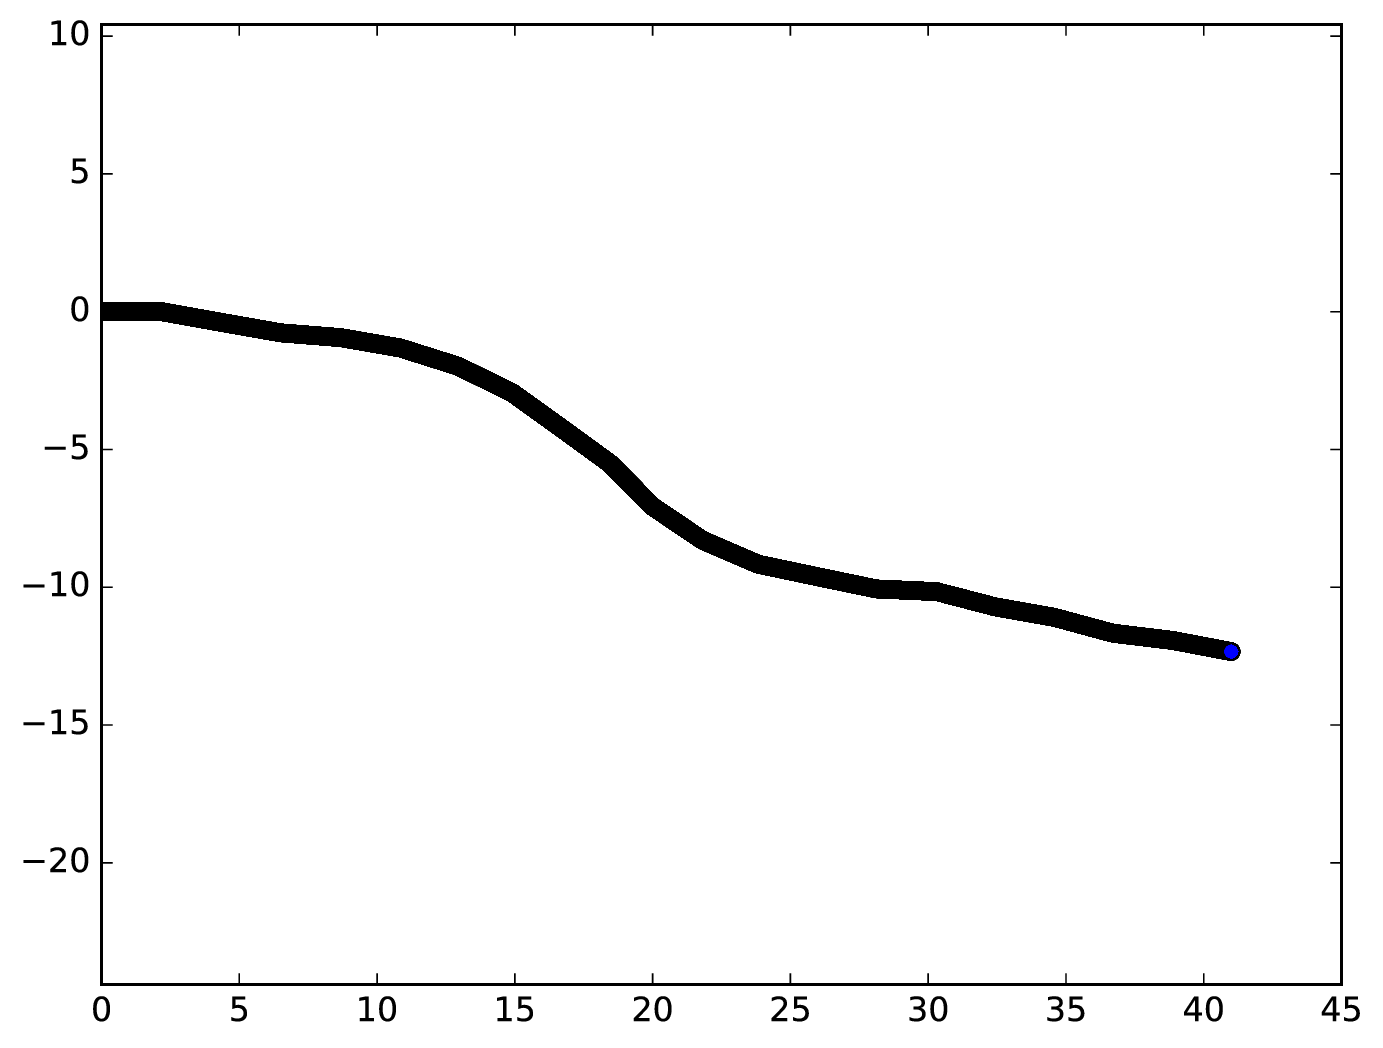
\includegraphics[width=\textwidth]{figures/ch3/synTraj_219_15_1}
			\caption[$A = 15$, $F=1$]{$A = 15$, $F=1$}
			\label{fig:synTraj_219_15_1}
		\end{subfigure}
		~
		\begin{subfigure}[t]{\subImgWmo}
			\centering
			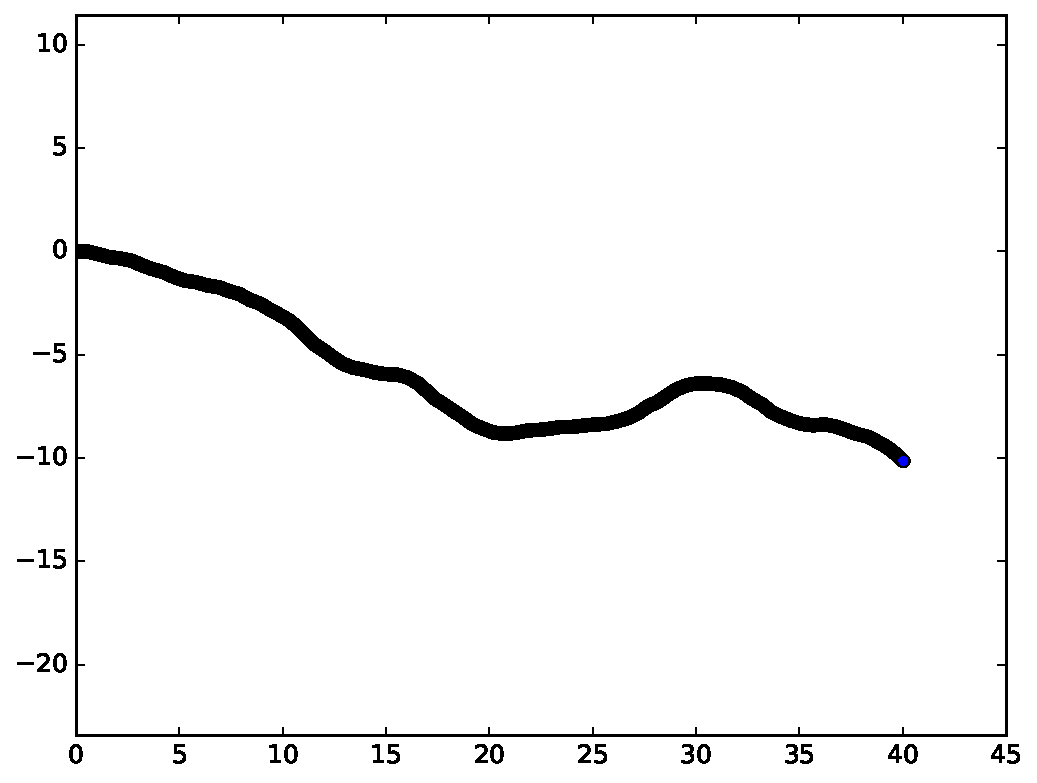
\includegraphics[width=\textwidth]{figures/ch3/synTraj_219_15_4}
			\caption[$A = 15$, $F=4$]{$A = 15$, $F=4$}
			\label{fig:synTraj_219_15_4}
		\end{subfigure}
		~
		\begin{subfigure}[t]{\subImgWmo}
			\centering
			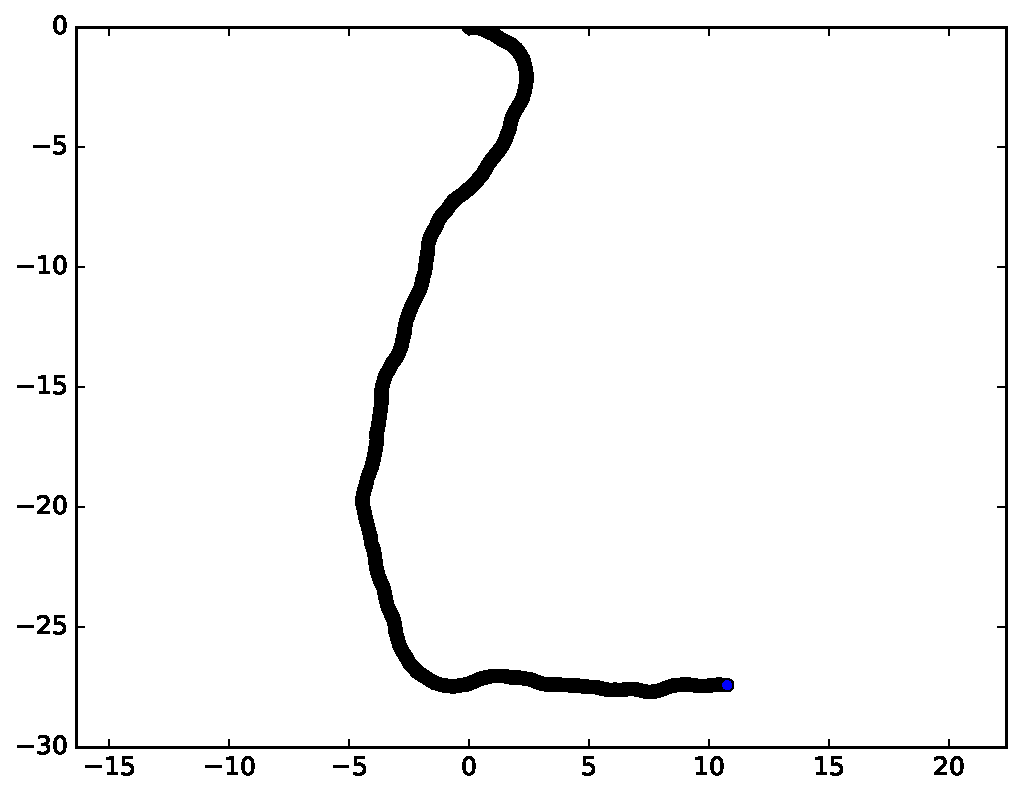
\includegraphics[width=\textwidth]{figures/ch3/synTraj_219_15_8}
			\caption[$A = 15$, $F=8$]{$A = 15$, $F=8$}
			\label{fig:synTraj_219_15_8}
		\end{subfigure}
		~
		\begin{subfigure}[t]{\subImgWmo}
			\centering
			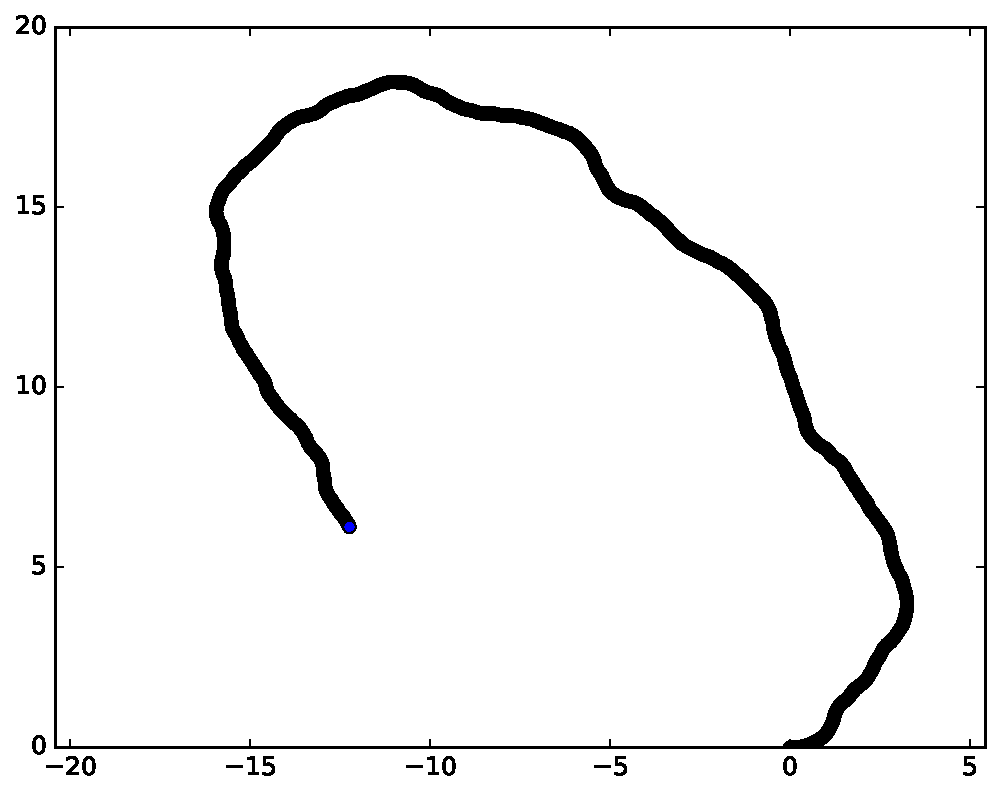
\includegraphics[width=\textwidth]{figures/ch3/synTraj_219_15_16}
			\caption[$A = 15$, $F=16$]{$A = 15$, $F=16$}
			\label{fig:synTraj_219_15_16}
		\end{subfigure}
		~
		\begin{subfigure}[t]{\subImgWmo}
			\centering
			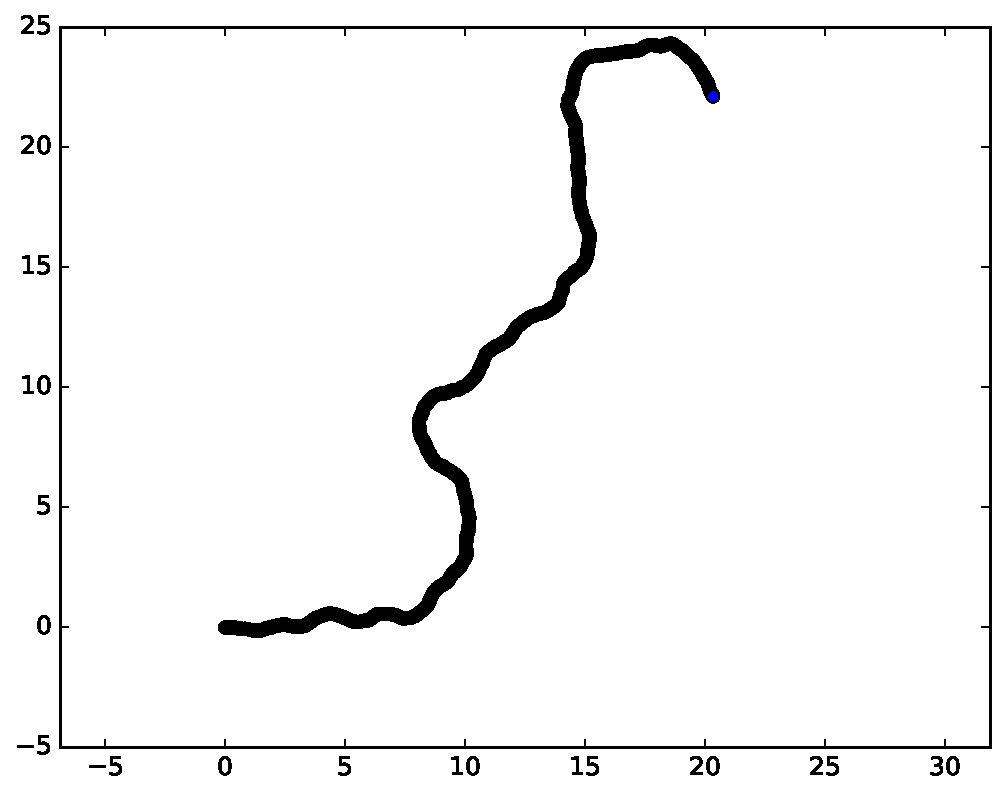
\includegraphics[width=\textwidth]{figures/ch3/synTraj_219_15_32}
			\caption[$A = 15$, $F=32$]{$A = 15$, $F=32$}
			\label{fig:synTraj_219_15_32}
		\end{subfigure}
		~
		\begin{subfigure}[t]{\subImgWmo}
			\centering
			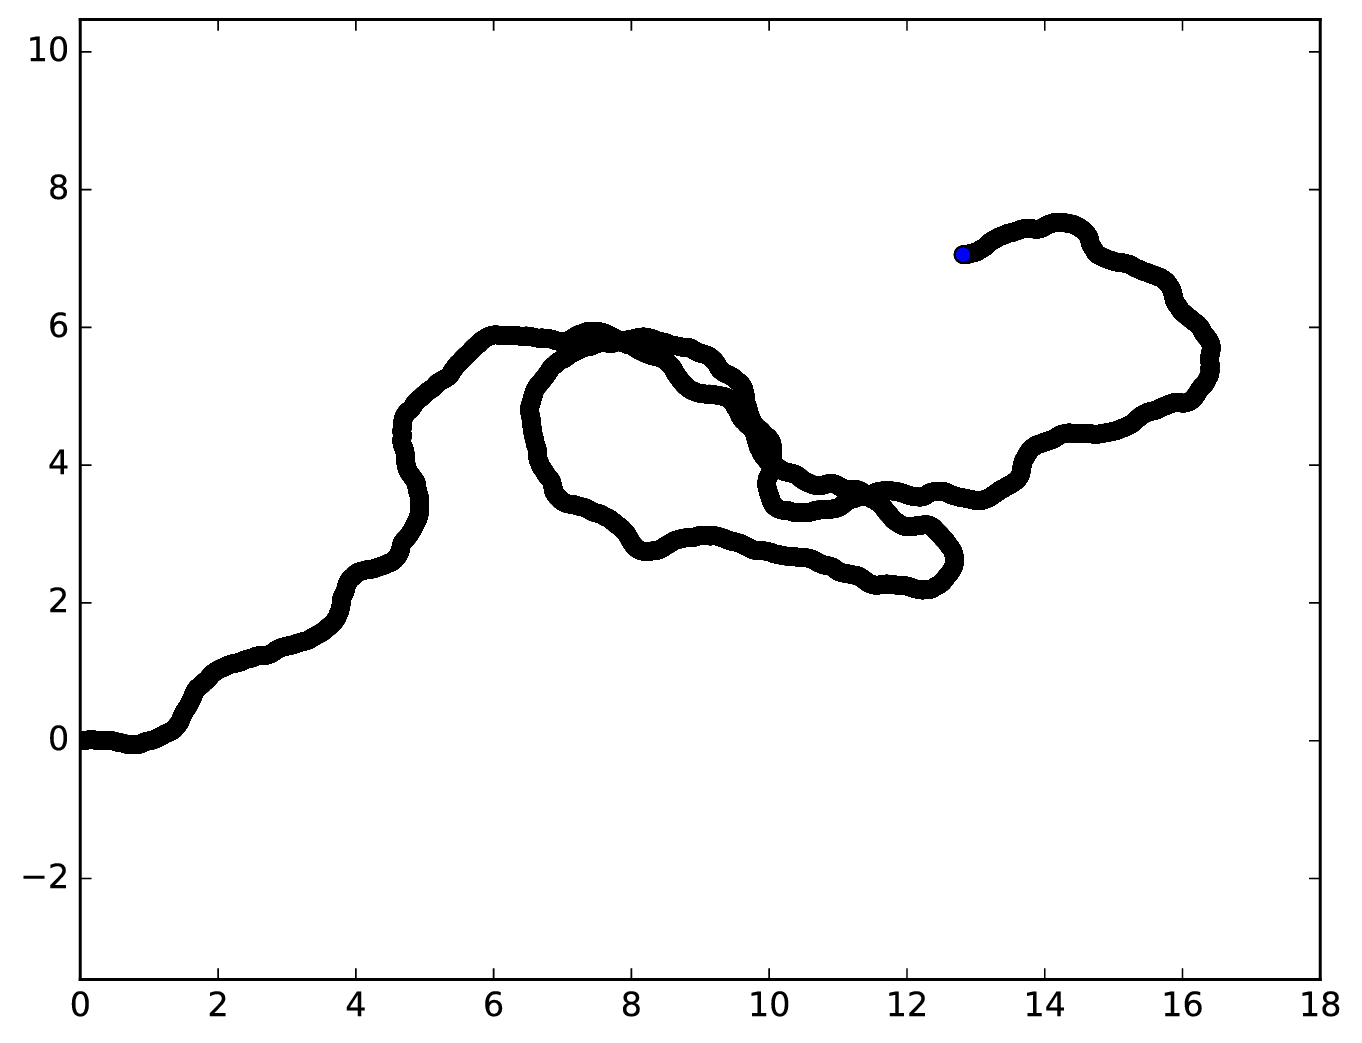
\includegraphics[width=\textwidth]{figures/ch3/synTraj_219_15_60}
			\caption[$A = 15$, $F=60$]{$A = 15$, $F=60$}
			\label{fig:synTraj_219_15_60}
		\end{subfigure}
		~
		\begin{subfigure}[t]{\subImgWmo}
			\centering
			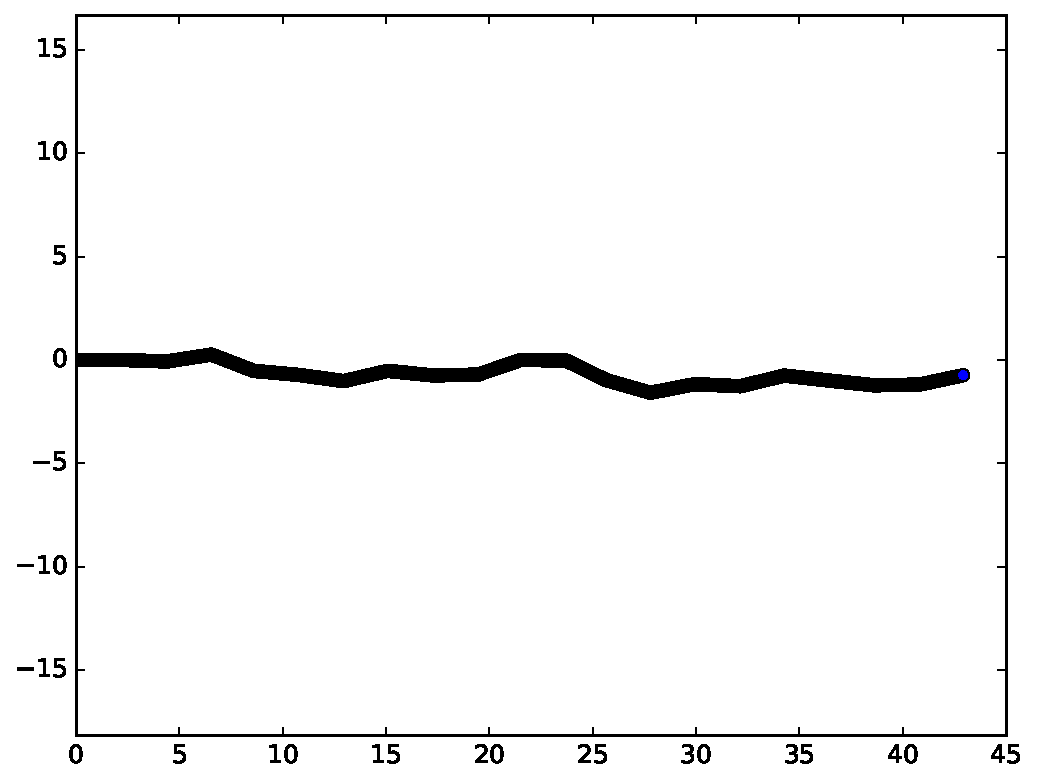
\includegraphics[width=\textwidth]{figures/ch3/synTraj_219_30_1}
			\caption[$A = 30$, $F=1$]{$A = 30$, $F=1$}
			\label{fig:synTraj_219_30_1}
		\end{subfigure}
		~
		\begin{subfigure}[t]{\subImgWmo}
			\centering
			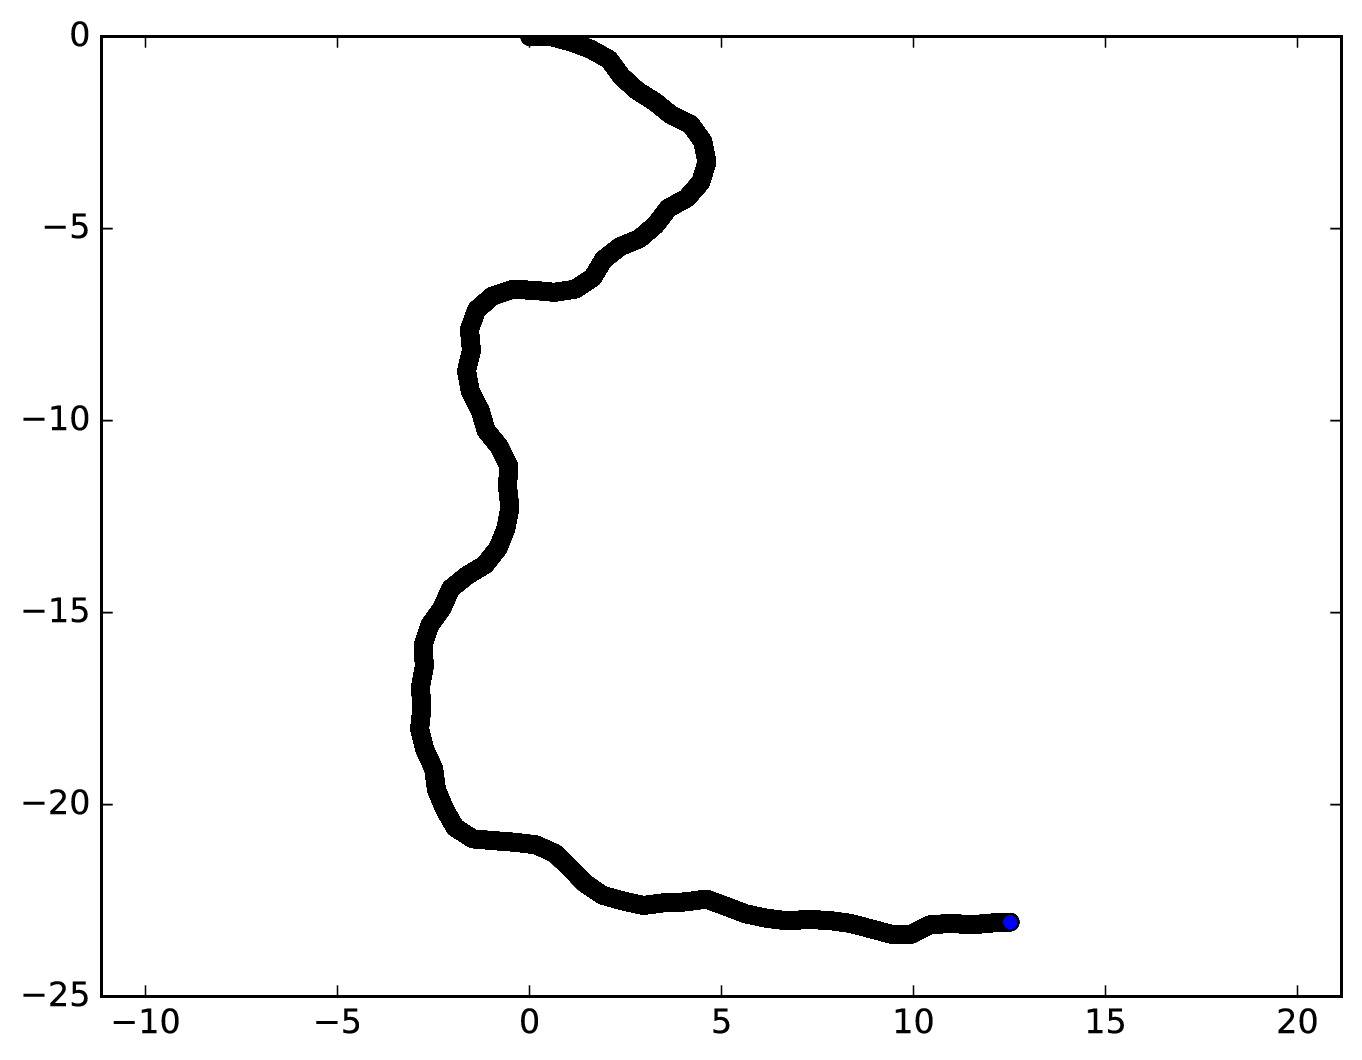
\includegraphics[width=\textwidth]{figures/ch3/synTraj_219_30_4}
			\caption[$A = 30$, $F=4$]{$A = 30$, $F=4$}
			\label{fig:synTraj_219_30_4}
		\end{subfigure}
		~
		\begin{subfigure}[t]{\subImgWmo}
			\centering
			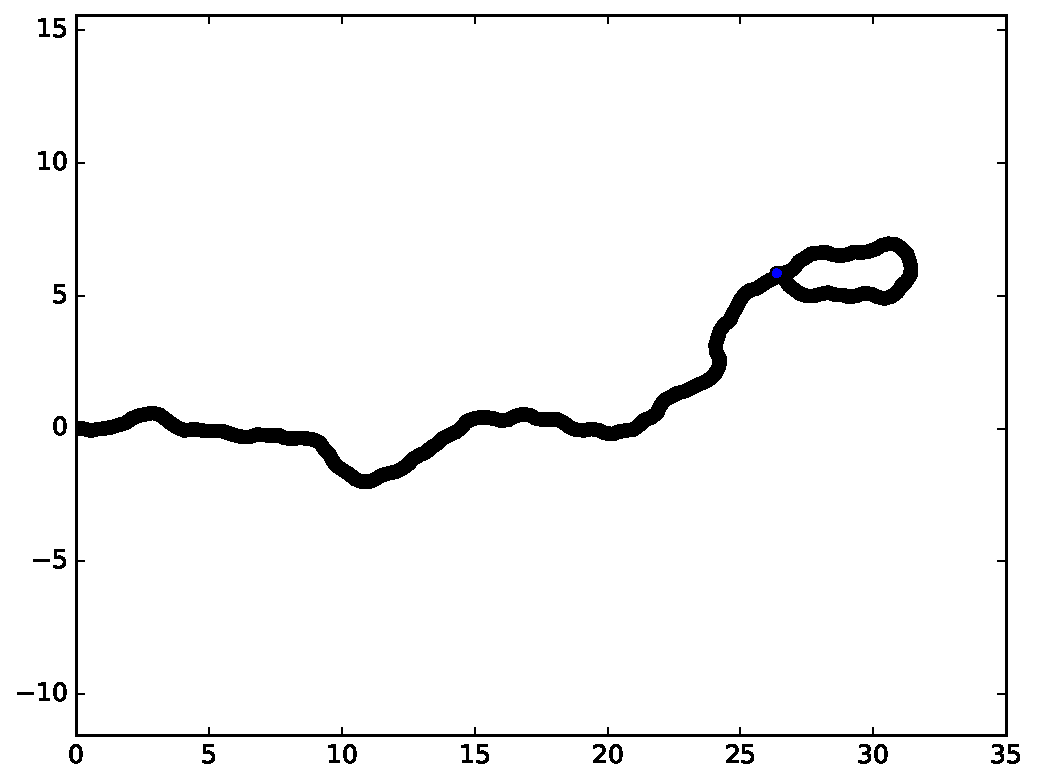
\includegraphics[width=\textwidth]{figures/ch3/synTraj_219_30_8}
			\caption[$A = 30$, $F=8$]{$A = 30$, $F=8$}
			\label{fig:synTraj_219_30_8}
		\end{subfigure}
		~
		\begin{subfigure}[t]{\subImgWmo}
			\centering
			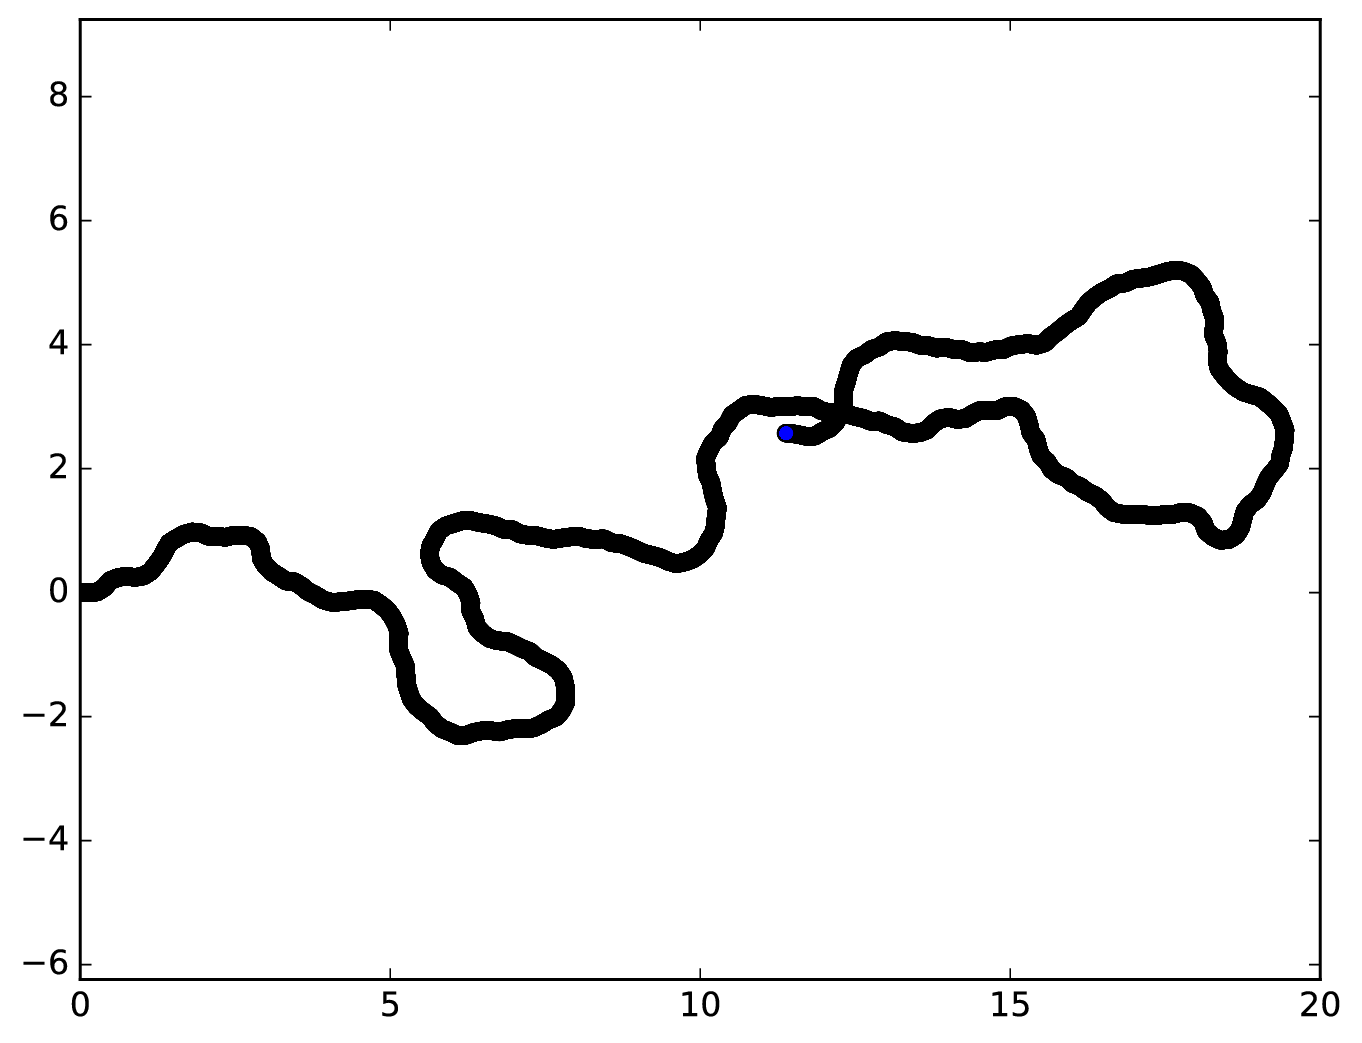
\includegraphics[width=\textwidth]{figures/ch3/synTraj_219_30_16}
			\caption[$A = 30$, $F=16$]{$A = 30$, $F=16$}
			\label{fig:synTraj_219_30_16}
		\end{subfigure}
		~
		\begin{subfigure}[t]{\subImgWmo}
			\centering
			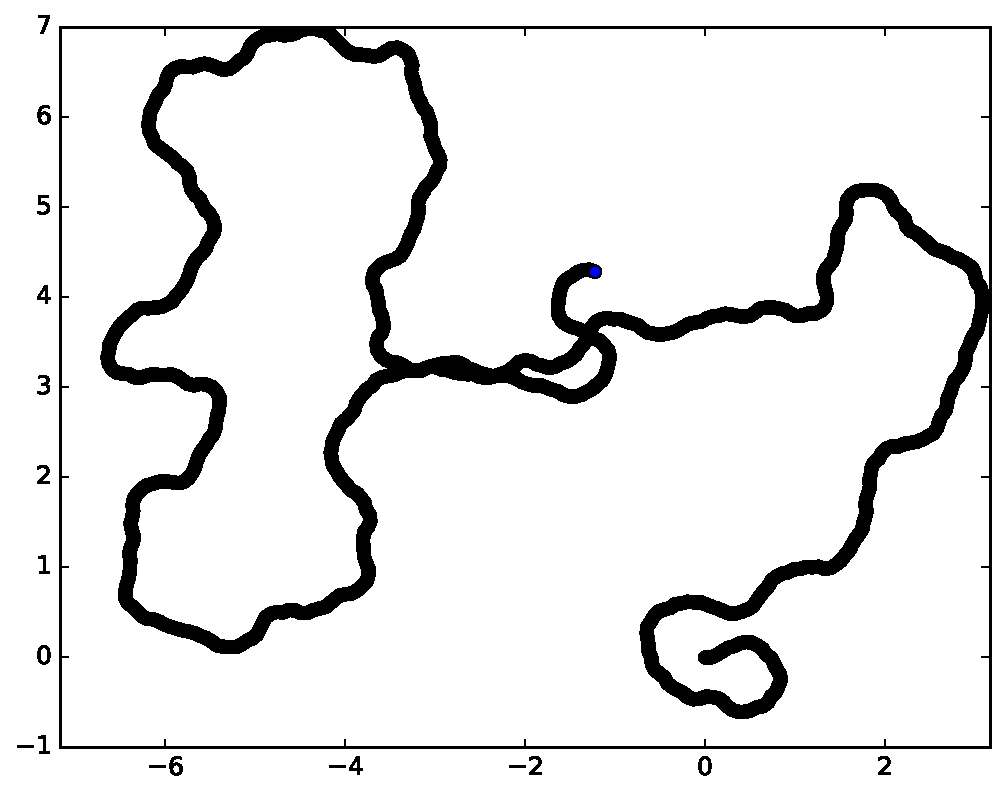
\includegraphics[width=\textwidth]{figures/ch3/synTraj_219_30_32}
			\caption[$A = 30$, $F=32$]{$A = 30$, $F=32$}
			\label{fig:synTraj_219_30_32}
		\end{subfigure}
		~
		\begin{subfigure}[t]{\subImgWmo}
			\centering
			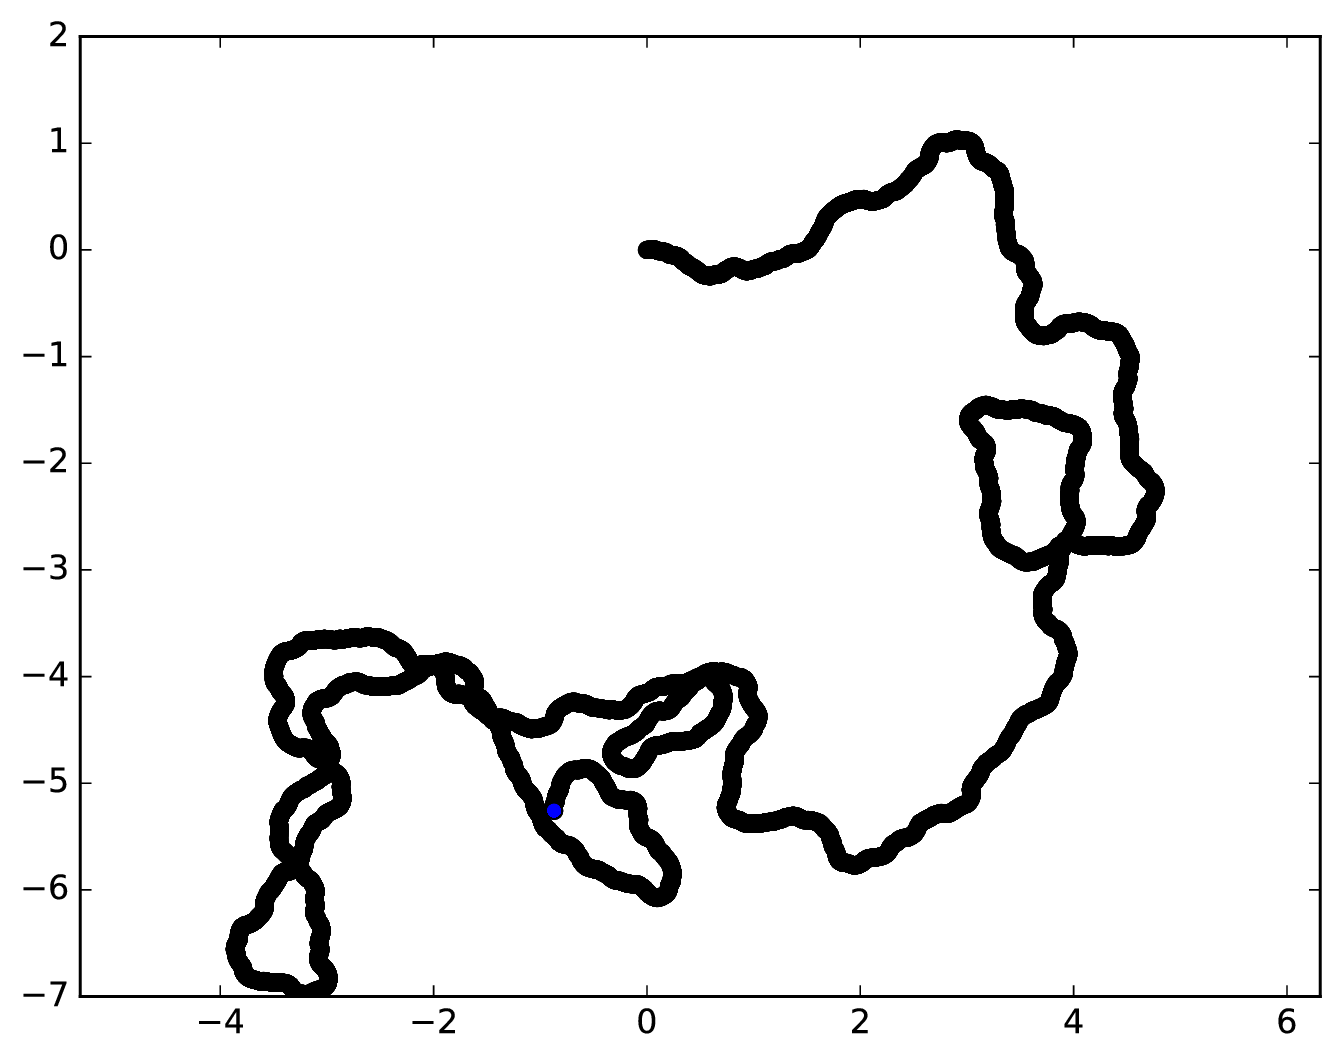
\includegraphics[width=\textwidth]{figures/ch3/synTraj_219_30_60}
			\caption[$A = 30$, $F=60$]{$A = 30$, $F=60$}
			\label{fig:synTraj_219_30_60}
		\end{subfigure}
		\caption[Mouvements générés par notre modèle]{Exemples de trajectoires générées par notre modèle pour un objet de vitesse constante (2,19~cm/s).}
		\label{fig:motion1530}
	\end{figure}
	
    \subsection{Un modèle puissant mais limité}
	Les capacités offertes par le modèle VFA sont très nombreuses, mais demeurent limitées, et ne peuvent couvrir tous les besoins en matière de génération de mouvement aléatoire.
    
    \subsubsection{Vitesse constante}
    Faire varier les paramètres, en particulier $F$ et $A$, permet de générer des types de mouvement subjectivement très différents. Néanmoins, et outre le problème des objets autocorrélés, notre modèle repose notamment sur une vitesse constante, ce qui, de fait, exclut tous les objets susceptibles d'accélérer. Là encore, ce choix fut fait pour limiter le nombre de paramètres, toujours dans l'objectif d'atteindre un compromis entre la simplicité du modèle et sa capacité à générer des mouvements que nos sujets puissent percevoir comme fondamentalement différents. Nous souhaitions tout particulièrement pouvoir générer du mouvement perçu comme \og régulier \fg{} ou \og prévisible \fg{} ainsi que du mouvement \og irrégulier \fg{}, \og saccadé \fg{} ou \og imprévisible \fg{}.
    
	\subsubsection{Pas de véritable autocorrélation}
	De même, ce modèle ne peut générer que du mouvement markovien. En effet, une rotation de $\vec{dir}$ générée est totalement indépendante de la dernière rotation générée, si elle existe. Cela ne signifie pas que $\vec{dir}_{t+1}$ soit indépendant de $\vec{dir}_{t}$, et il ne l'est pas, mais que le \emph{changement} de direction à tout instant est indépendant du passé de l'objet concerné. Il en résulte que ce modèle ne peut générer du mouvement autocorrélé. Ce choix reflète d'une part notre focus originel sur les simulations moléculaires (où il y a une demande claire émanant des utilisateurs) et d'autre part une volonté de conserver un modèle aussi simple que possible, afin de le rendre plus facile à utiliser, mais aussi pour pouvoir évaluer un échantillon représentatif des types de mouvements qu'il peut générer dans un laps de temps raisonnable pour une étude empirique, compte tenu notamment de la fatigue des sujets.
    
    \paragraph{Mouvements pseudo-autocorrélés.}
    \label{sub:pseudoAutoCorr}
	Néanmoins, une trajectoire générée par notre modèle peut, au moins temporairement, approximer un mouvement autocorrélé. Attendu qu'une tâche de sélection, pour peu qu'elle ne soit pas trop difficile, peut se dérouler sur une durée inférieure ou égale à la durée pendant laquelle le modèle VFA peut approximer un mouvement autocorrélé, il n'est pas inutile pour étudier les performances de sélection de ces objets. On privilégiera dans ce cas de très fortes valeurs de $F$ et de très faibles valeurs de $A$. La figure~\ref{fig:autocorr} fournit deux exemples de telles trajectoires que nous proposons d'appeler pseudo-autocorrélées, générées avec $F \in \{30,120\}$ et $A \in \{1,2\}$.
	
	\begin{figure}[!htb]
		%\centering
		\begin{subfigure}[t]{0.23\textwidth}
			\centering
			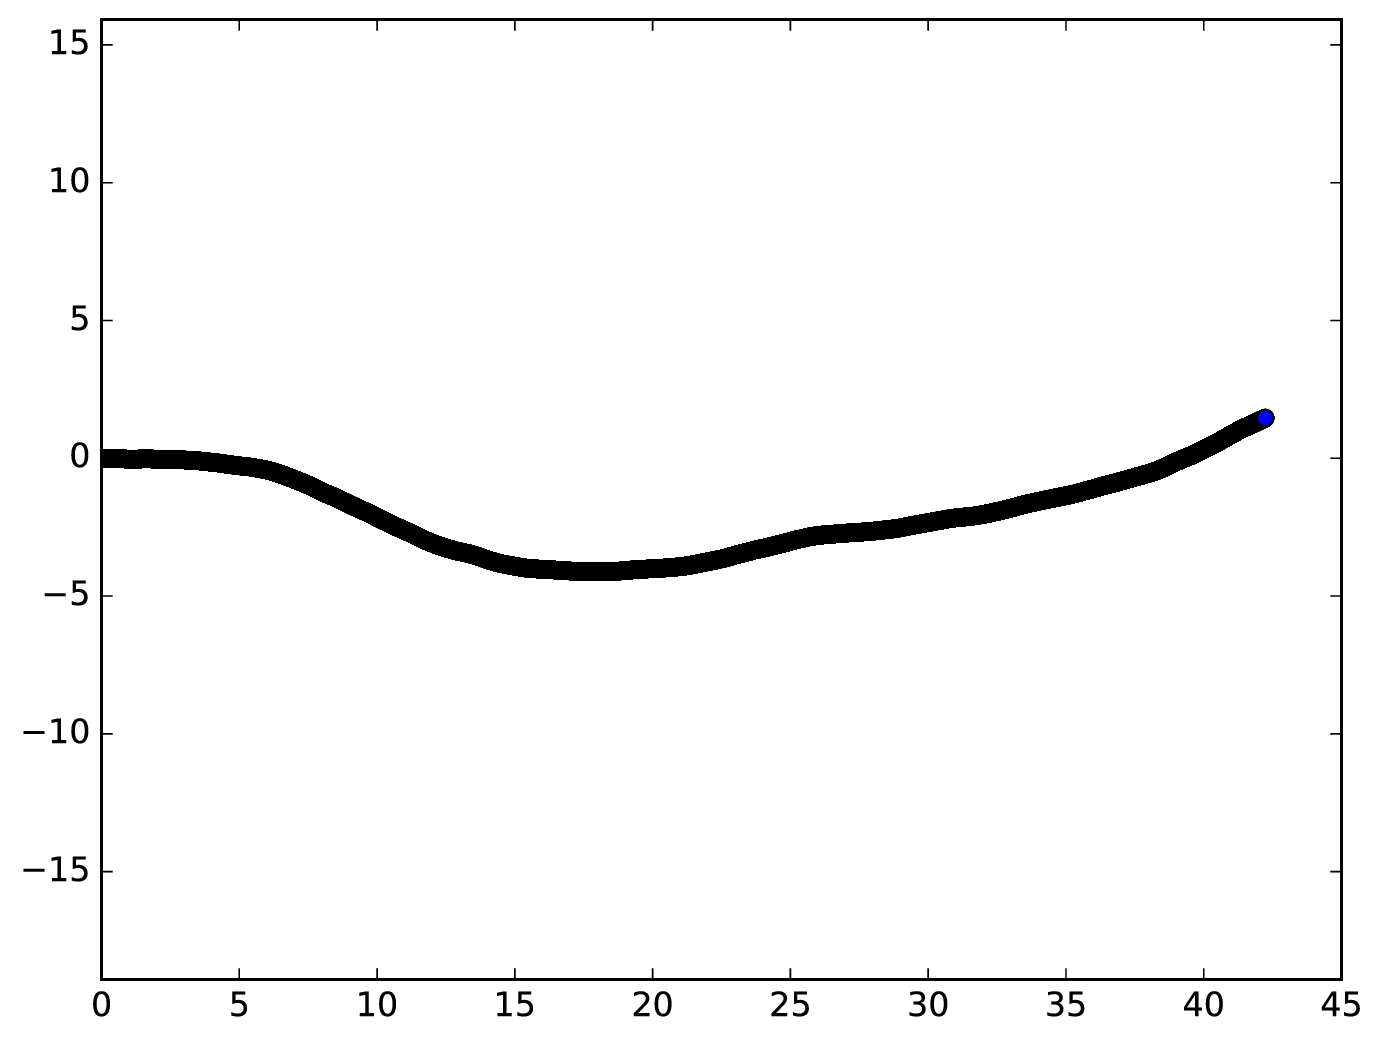
\includegraphics[width=\textwidth]{figures/ch3/ac_2_19_1_120a}
			\caption{$F=120$ ; $A=1$.}
			\label{fig:ac1_120A}
		\end{subfigure}
		~
		\begin{subfigure}[t]{0.23\textwidth}
			\centering
			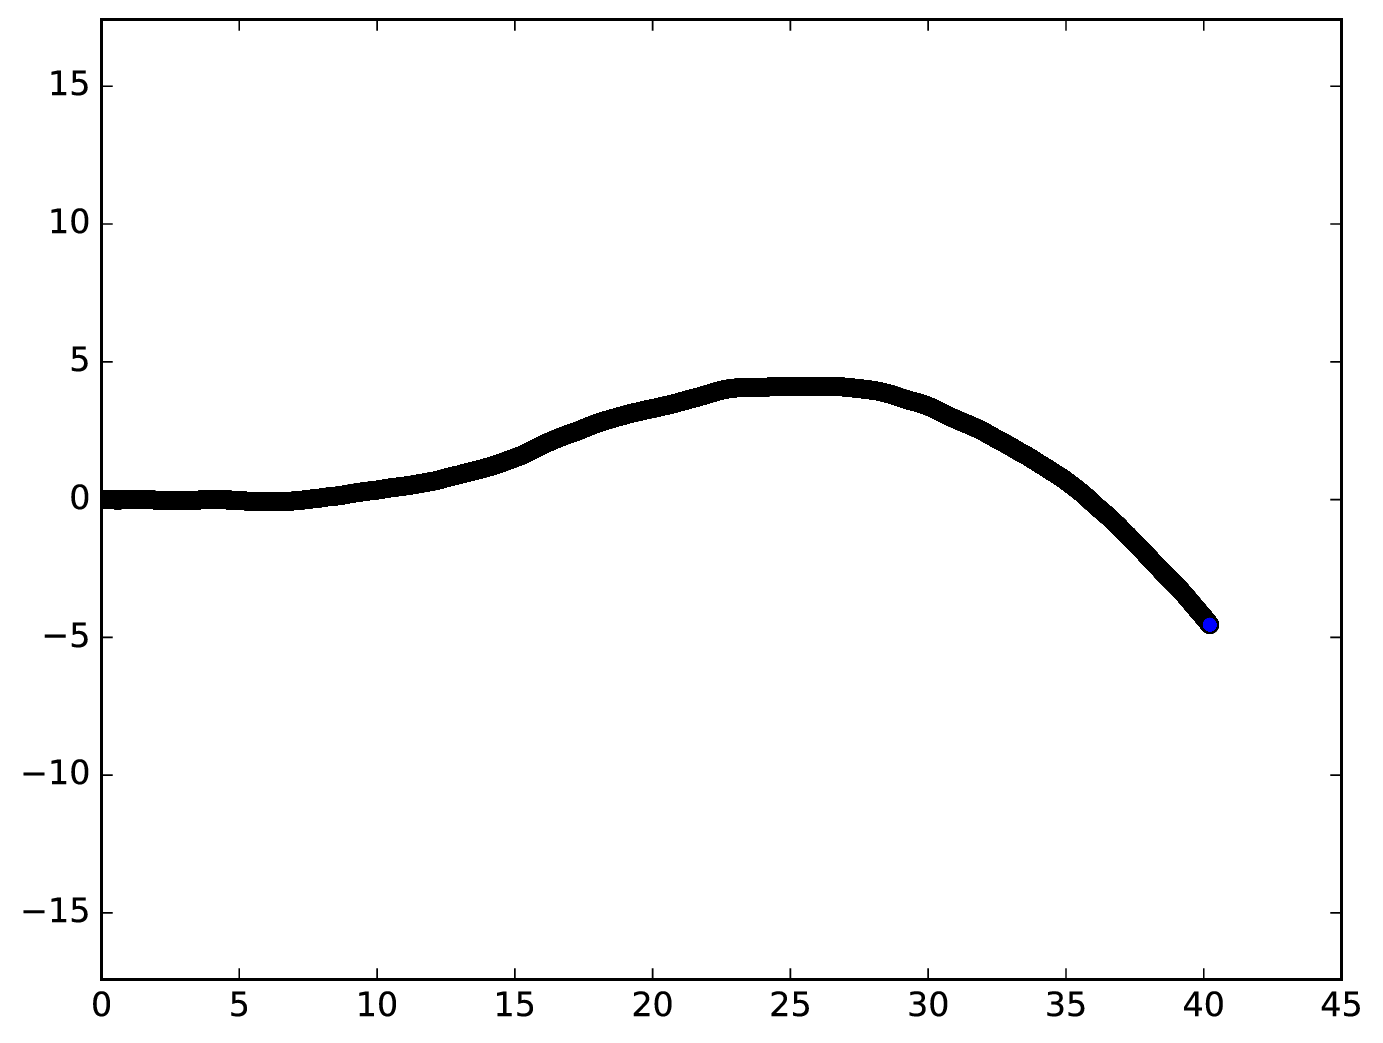
\includegraphics[width=\textwidth]{figures/ch3/ac_2_19_1_120b}
			\caption{$F=120$ ; $A=1$, bis.}
			\label{fig:ac_1_120B}
		\end{subfigure}
		~
		\begin{subfigure}[t]{0.23\textwidth}
			\centering
			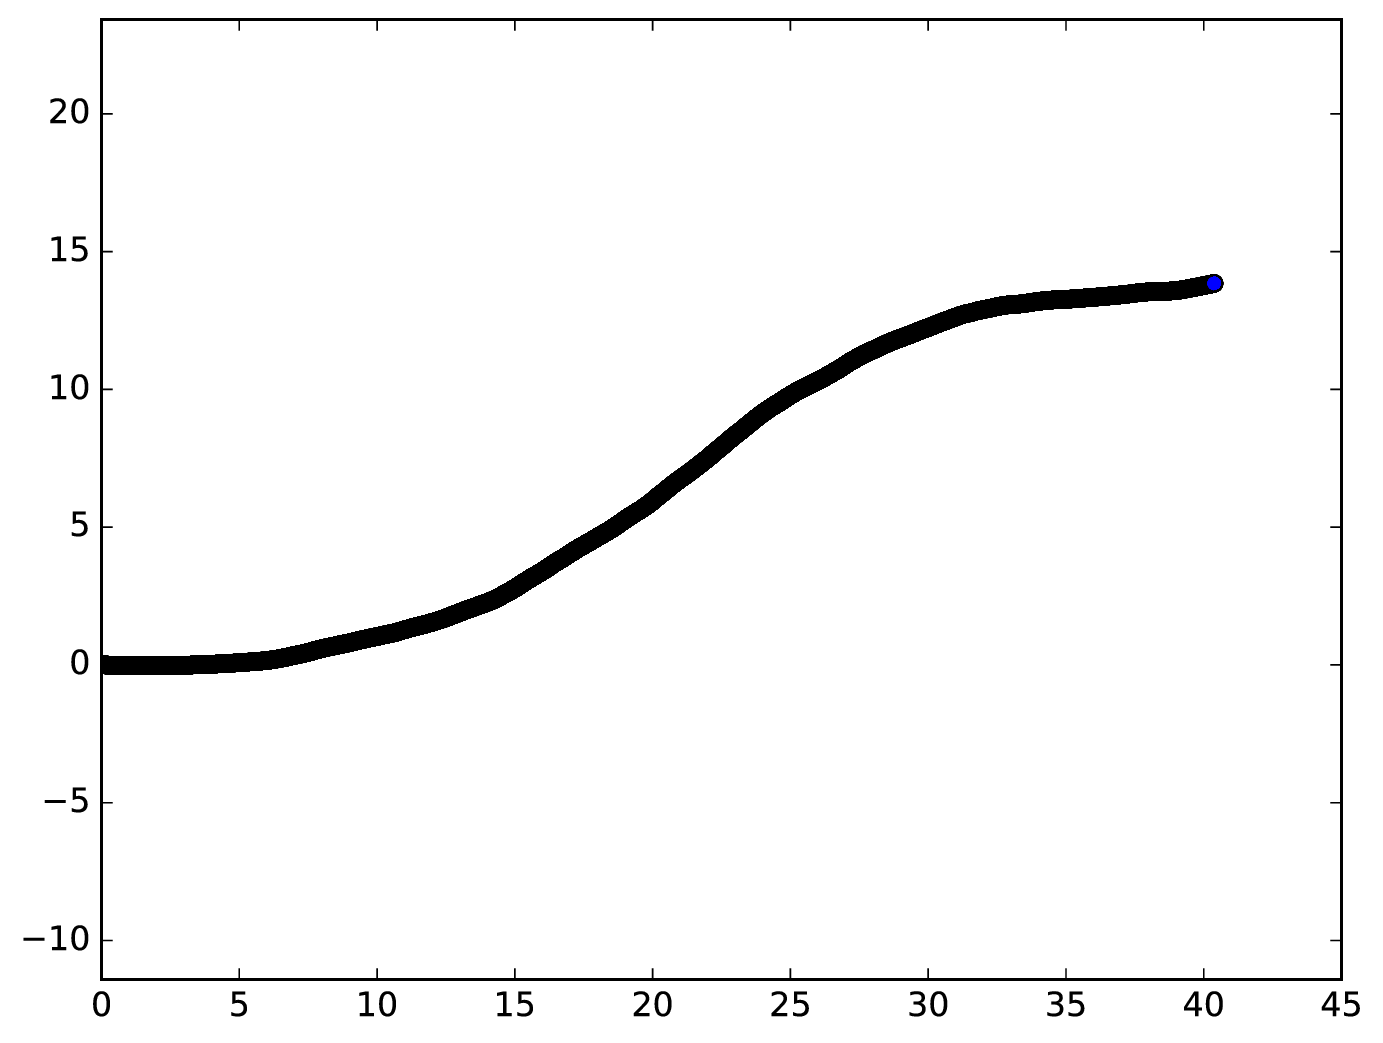
\includegraphics[width=\textwidth]{figures/ch3/ac_2_19_2_30}
			\caption{$F=30$ ; $A=2$.}
			\label{fig:ac_2_30}
		\end{subfigure}		
		~
		\begin{subfigure}[t]{0.23\textwidth}
			\centering
			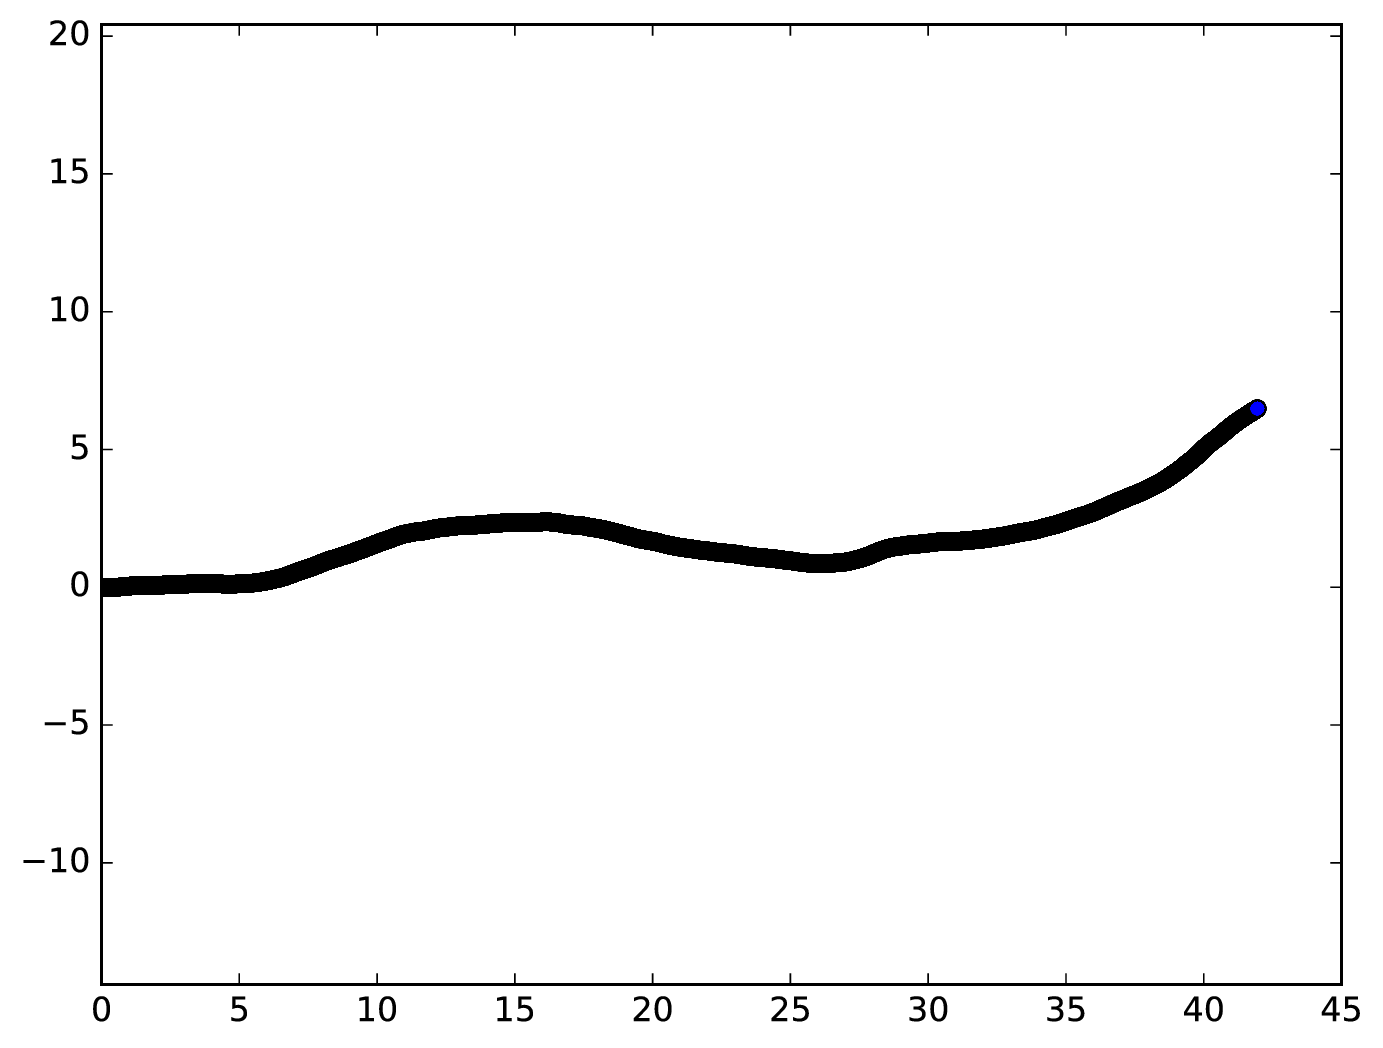
\includegraphics[width=\textwidth]{figures/ch3/ac_2_19_2_60}
			\caption{$F=120$ ; $A=1$, ter.}
			\label{fig:ac_1_120C}
		\end{subfigure}
		\caption[Mouvements pseudo-autocorrélés]{Trois trajectoires générées avec les mêmes valeurs $F = 120$~Hz et $A = 1\degree$, et une avec $F = 30$~Hz et $A = 2\degree$ ; dans tous les cas, $V = 2,19$~cm/s. Elles ressemblent à celles d'objets autocorrélés, comme des véhicules.}
		\label{fig:autocorr}
	\end{figure}
    
    \subsection{Modèles de génération de mouvements autocorrélés}
    \label{sub:vfaAutoCorr}
    Les objets autocorrélés présentent néanmoins un intérêt certain, et les trajectoires pseudo-autocorrélées ne sont que des approximations qui peuvent s'avérer insuffisantes. Nous proposons donc ici deux modèles différents permettant de générer des mouvements réellement autocorrélés.
    
    \subsubsection{Modèle VFA à mémoire}
    \label{sub:vfaMem}
    Une première option pour un modèle adapté aux objets autocorrélés serait d'adapter le modèle VFA en lui ajoutant une mémoire, par exemple une mémoire du dernier changement de direction de l'objet concerné. L'on retiendrait ainsi l'angle du changement de direction à l'instant précédent ($\alpha_{t-T}$, avec $T = \frac{1}{F}$), et l'on pourrait appliquer un nouveau changement avec un angle plus ou moins proche de ce dernier, selon des paramètres. L'équation~\ref{eq:vfamem} présente une possibilité, où $\alpha$ est échantillonné entre $-A$ et $+A$, et $c_{ac} \in [0,1]$ est un coefficient d'autocorrélation.
    
    \begin{equation}
		\alpha_{t} = \alpha_{t-T} \times c_{ac} + \alpha (1 - c_{ac})
		\label{eq:vfamem}
    \end{equation}
    
	Ainsi, lorsque le coefficient d'autocorrélation est nul, le système devient markovien ; lorsqu'il vaut 1, $\alpha_{nT}$ est constant (avec $n \in \mathbb{N}$). De fait, s'il est non nul, l'objet aura un mouvement circulaire s'il est ciné-continu, et régulier s'il est ciné-discret ; s'il est nul, le mouvement sera rectiligne dans les deux cas. Les figures~\ref{fig:realAutocorr} et~\ref{fig:realAutocorr2} fournissent des illustrations de mouvements autocorrélés générés par ce modèle, avec divers coefficients de corrélation, de 0 à 100~\%{}. La valeur initiale de l'angle de rotation du vecteur vitesse choisie ici est nulle, d'où un mouvement rectiligne quand le coefficient vaut 100~\%{}.
	
	Notez que nous fournissons plus d'exemples avec des coefficients proches de 100~\%{} car ce sont eux qui fournissent les résultats les plus proches de mouvements d'objets macroscopiques familiers. Ici, le rapport $\frac{F}{V}$ est suffisamment élevé pour que les mouvements semblent continus lorsque $c_{ac}$ est élevé. Ajoutons qu'avec une valeur de A plus faible, ce coefficient n'aurait pas besoin d'être si élevé pour générer de telles trajectoires.
    
    \subsubsection{Modèle newtonien}
    Une seconde option ayant un certain sens physique consisterait à considérer chaque objet comme une particule dotée d'une masse, et de la soumettre à une force qui, elle, serait régie par un modèle de type VFA, éventuellement modifié pour remplacer la vitesse par la norme de la force, notamment. Il serait opportun d'appliquer une force de friction afin d'éviter que l'application continue d'une force (et donc d'une accélération\footnotemark{}) ne mène à des vitesses croissantes et non bornées.
    
    \footnotetext{Rappelons que, d'après la seconde loi de Newton~\cite{newton1833philosophiae}, $\vec{F} = m\vec{a}$ où $F$ est une force, $m$ est la masse de l'objet sur lequel elle agit, et $\vec{a}$ est l'accélération de l'objet, soit $\vec{a} = \frac{\vec{F}}{m}$ : sans friction, l'accélération est constante et la vitesse diverge.}
    
    Le modèle nécessiterait un calibrage précis pour obtenir le comportement souhaité, notamment en ce qui concerne les masses des objets ou le coefficient de friction. Par ailleurs, sauf dans certains cas particuliers (et après une période dynamique) les vitesses des objets ne seraient pas constantes pour une norme de $\vec{F}$ donnée, ce qui distinguerait ce modèle newtonien du nôtre (VFA). En soi, ce n'est pas nécessairement un problème --- et peut même être un avantage --- mais cela complique le contrôle des propriétés d'un environnement synthétique créé pour mener une étude empirique.
	
	\subsection{Entropie}
	La discussion des facteurs qui déterminent la nature du mouvement, et en particularité sa régularité, amène à considérer la question de l'ordre et du désordre dans le mouvement. Ces propriétés pourraient en effet avoir une influence sur la difficulté d'anticipation de la trajectoire d'une cible, et donc de sa sélection.
	
	Dans ses travaux sur la thermodynamique, Clausius définit l'entropie comme \og le contenu de transformation [d'un] corps \fg{}~\cite{clausius1865verschiedene, clausius1865diverses}. Rapidement, Boltzmann redéfinit l'entropie $S$ par l'équation $S = k\log(W)$, où $k$ est une constante et $W$ est le nombre d'états dans lequel un système peut se trouver~\cite{boltzmann1866mechanische, weisstein2004eric}. À partir de la définition de Boltzmann, Claude Shannon redéfinit à nouveau l'entropie~\cite{shannon1949communication} comme une fonction $H(X)$ dépendant d'une variable aléatoire discrète $X$ de valeurs possibles $\{x_{1}, \ldots{}, x_{n}\}$ (voir l'équation~\ref{eq:shannonEntropy}, où $P(x_{i})$ est la probabilité que $X=x_{i}$).
	
	\begin{equation}
		\label{eq:shannonEntropy}
		H(X) = -\sum_{i=1}^{n}P(x_{i})\log_{b}\left(P(x_{i})\right)
	\end{equation}
	
	L'on peut toutefois écrire cette équation de façon plus succincte --- et peut-être plus parlante --- comme dans l'équation~\ref{eq:shaEnt}, où $I(X)$ est la quantité d'information de $X$, et $E[I(X)]$ est l'espérance de cette quantité. Notez que $I(e) = -\log\left(P(e)\right)$, où $e$ est un événement.
	
	\begin{equation}
		\label{eq:shaEnt}
		H(X) = E[I(X)]
	\end{equation}
	
	En résumé, pour Shannon, l'entropie d'une variable croît avec sa quantité d'information, et celle-ci est d'autant plus grande que les événements possibles sont rares. Si l'on suppose qu'ils sont équiprobables, alors ils sont d'autant plus rares qu'ils sont nombreux. Dans le cas qui nous concerne, on peut donc dire qu'une cible est de forte entropie si, pour une position donnée à l'instant $t$, les positions possibles à l'instant $t+1$ sont nombreuses (en les supposant équiprobables).
	
	Supposons donc une cible de position $pos$ et de vecteur vitesse $\vec{dir}$ à l'instant $t$. Si $F=0$ ou $A=0$, alors $pos_{t+1} = pos + S \times \vec{dir}$. Seul cet état est possible, donc la quantité d'information de la cible est nulle, et son entropie aussi. En revanche, s'il peut y avoir une rotation de $\vec{dir}$ à l'instant $t+1$, alors l'entropie sera non nulle, et dépendra de la probabilité de ce changement de direction, ainsi que du nombre de valeurs possibles pour le changement de direction $\alpha$.
	
	Si l'on considère $\alpha$ comme un nombre réel, le nombre de valeurs possibles est infini, et l'entropie aussi. Mais pour un utilisateur, un changement de direction de 10,0001\textdegree{} n'est probablement pas différent d'un changement de 10\textdegree{} ; aussi serait-il judicieux de discrétiser l'espace de $\alpha$. Une solution consiste à arrondir la valeur à l'entier le plus proche, ce qui réduit l'espace aux entiers contenus dans l'intervalle $]-180\degree{}, +180\degree{}]$, soit 360 valeurs.
	
	La portion de cet espace effectivement possible dépend de $A$ ; plus précisément, elle vaut $\frac{A}{180}$. L'on peut donc calculer l'entropie d'une cible si l'on connaît $A$ et si l'on sait qu'il y aura un changement de direction à l'instant suivant, mais ce calcul ne vaudra que sur une fenêtre temporelle limitée à deux \og instants \fg{} --- ce qui implique d'ailleurs une discrétisation du temps, potentiellement indésirable.
	
	Pour connaître l'entropie globale $E_{g}$ de la cible, on peut poser que $E_{g}$ est la moyenne des $E_{t}$ pour chaque instant $t$. Si l'on suppose que le temps est discrétisé de telle manière qu'un instant vaut $\frac{1}{60}$~s, alors $E_{g} = E_{t_{c}} \frac{F}{60}$ où $E_{t_{c}}$ est l'entropie de la cible à l'instant d'un changement de direction sûr.
	
	Or, ce calcul d'entropie dépend d'hypothèses parfois très fortes :
	
	\begin{itemize}
		\item $A$ est connu ;
		\item $F$ est connu ;
		\item Pour une valeur de $A$ donnée, tous les $\alpha$ sont équiprobables ;
		\item La discrétisation de l'espace des $\alpha$ ne fausse pas l'estimation de l'entropie, c'est-à-dire qu'elle n'est ni trop fine ni trop grossière ;
		\item La discrétisation du temps ne fausse pas l'estimation de l'entropie, c'est-à-dire qu'elle n'est ni trop fine ni trop grossière.
	\end{itemize}
	
	\subsubsection{Pseudo-entropie.}	
	Pour simplifier le problème, l'on peut simplement remarquer que :
	\begin{itemize}
		\item Plus $F$ est élevé, plus la direction change souvent,
		\item Plus $A$ est élevé, plus ces changements peuvent être importants,
		\item Les trajectoires observées sur les figures~\ref{fig:motion1530}, \ref{fig:motion4560}, \ref{fig:motion7590}, \ref{fig:motion105120}, \ref{fig:motion135150} et \ref{fig:motion165180} révèlent que, souvent, une trajectoire avec une valeur de $A$ relativement basse et une valeur de $F$ relativement haute sera subjectivement semblable à une trajectoire avec une valeur de $A$ relativement haute et une valeur de $F$ relativement basse.
	\end{itemize}
	
	Il paraît donc raisonnable d'envisager le produit $AF$ comme une pseudo-entropie, et ce d'autant plus qu'il s'annule dès lors que $A=0$ ou $F=0$, de même que l'entropie. Il a en outre le mérite d'être très simple à calculer, d'autant que ce calcul est possible à partir de valeurs typiques et maximales estimées. Nous pouvons aisément déduire des observations faites plus haut sur F et A que l'entropie et la pseudo-entropie pourront être très élevées pour les objets ciné-discrets mais tendront à être faibles pour les objets ciné-continus (après discrétisation).
	
	Nous proposons ici un examen détaillé de quelques trajectoires. Avant tout autre propos, que le lecteur nous permette d'attirer son attention sur le fait que les trajectoires illustrées sur les figures~\ref{fig:motion1530}, \ref{fig:motion4560}, \ref{fig:motion7590}, \ref{fig:motion105120}, \ref{fig:motion135150} et \ref{fig:motion165180} sont représentées à des échelles différentes. En effet, la trajectoire de la figure~\ref{fig:synTraj_219_15_1} parcourt plus de 40~cm à l'horizontale, tandis que celle de la figure~\ref{fig:synTraj_219_180_60} est contenue dans un rectangle d'environ 1,2~cm de hauteur sur 1~cm de largeur.
	
	Il est donc inévitable de représenter ces trajectoires à des échelles adaptées si l'on souhaite qu'elles soient lisibles, mais il convient de faire attention à l'échelle et de garder à l'esprit que les trajectoires les plus irrégulières sont généralement représentées à une échelle bien plus petite.
	
	\subsubsection{Effet des vitesses}
	Modifier la vitesse d'un objet ne change pas la \og nature \fg{} du mouvement ni, au sens strict, son entropie. En effet, pour des valeurs de $A$ et $F$ données et une position donnée à l'instant $t$, le nombre d'états possible à l'instant $t+1$ ne dépend pas de la vitesse. On observe cependant qu'à mesure que la vitesse croît, une \og dilatation \fg{} des trajectoires s'opère, comme l'illustre la figure~\ref{fig:spEffect}, comparant diverses trajectoires générées avec des vitesses différentes mais des valeurs de $A$ et $F$ constantes.
	
	Il convient toutefois d'être prudent en interprétant cette donnée. En effet, si le nombre d'états possibles est objectivement le même, ces états ne sont pas nécessairement équivalents entre eux du point de vue subjectif d'un utilisateur tentant de sélectionner l'objet. En effet, si l'on suppose par exemple que l'objet en question est une sphère de 1~cm de diamètre, si elle se déplace à 0,5~cm/s, au bout d'une seconde une partie de l'objet sera toujours dans l'espace qu'il occupait à la seconde précédente ; pour une vitesse de 4~cm/s, ce n'est pas nécessairement le cas. La figure~\ref{fig:spTraj_0_5_120_2} montre qu'à basse vitesse (et à partir d'un certain niveau de pseudo-entropie) la cible évolue dans un espace très restreint ; inversement, quand la vitesse est élevée, comme sur la figure~\ref{fig:spTraj_4_0_120_2}, cette zone peut devenir très grande.
	
	Plus généralement, une cible d'une entropie donnée pourra s'éloigner d'autant plus rapidement du curseur de l'utilisateur que sa vitesse est élevée, et nous savons depuis les travaux de Fitts que la distance au curseur est déterminante pour la difficulté de sélection. Remarquons simplement ici, et avant d'analyser des données quantitatives précises, que si la vitesse d'un objet ne modifie pas son entropie, ces deux valeurs doivent être examinées conjointement pour (espérer) caractériser correctement la difficulté de sélection.	

	\begin{figure}[htb]
		\centering
		\begin{subfigure}[t]{\subImgWmo}
			\centering
			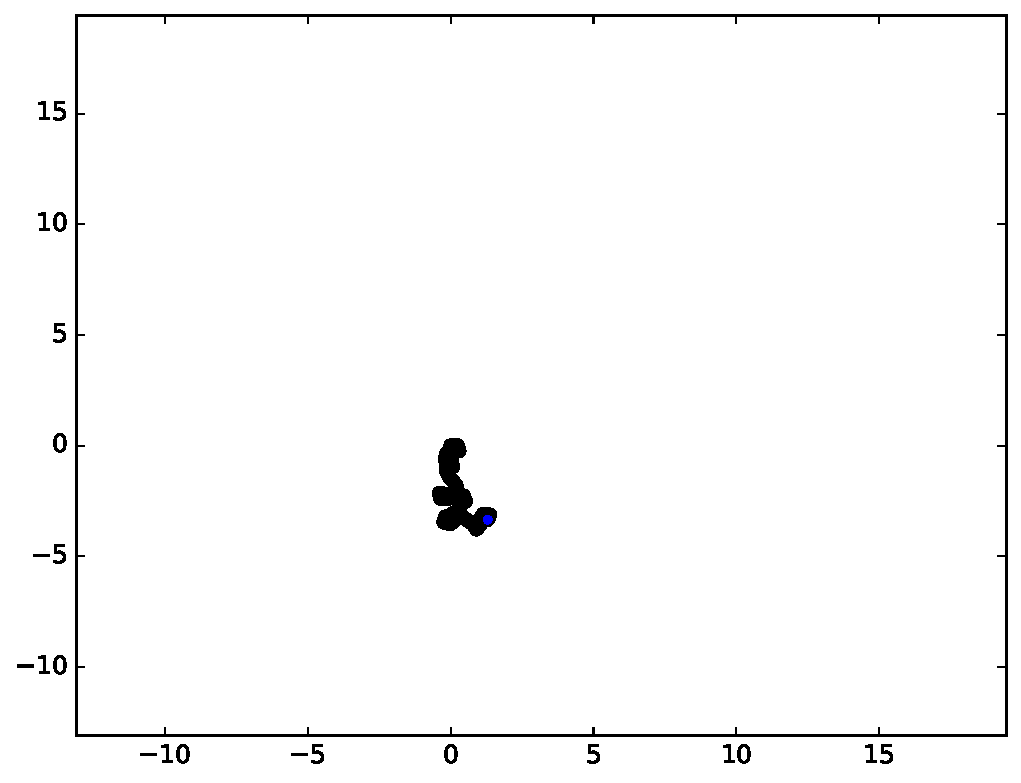
\includegraphics[width=\textwidth]{figures/ch3/spTraj_0_5_120_2}
			\caption[$S = 0,5$]{$S = 0,5$~cm/s.}
			\label{fig:spTraj_0_5_120_2}
		\end{subfigure}
		~
		\begin{subfigure}[t]{\subImgWmo}
			\centering
			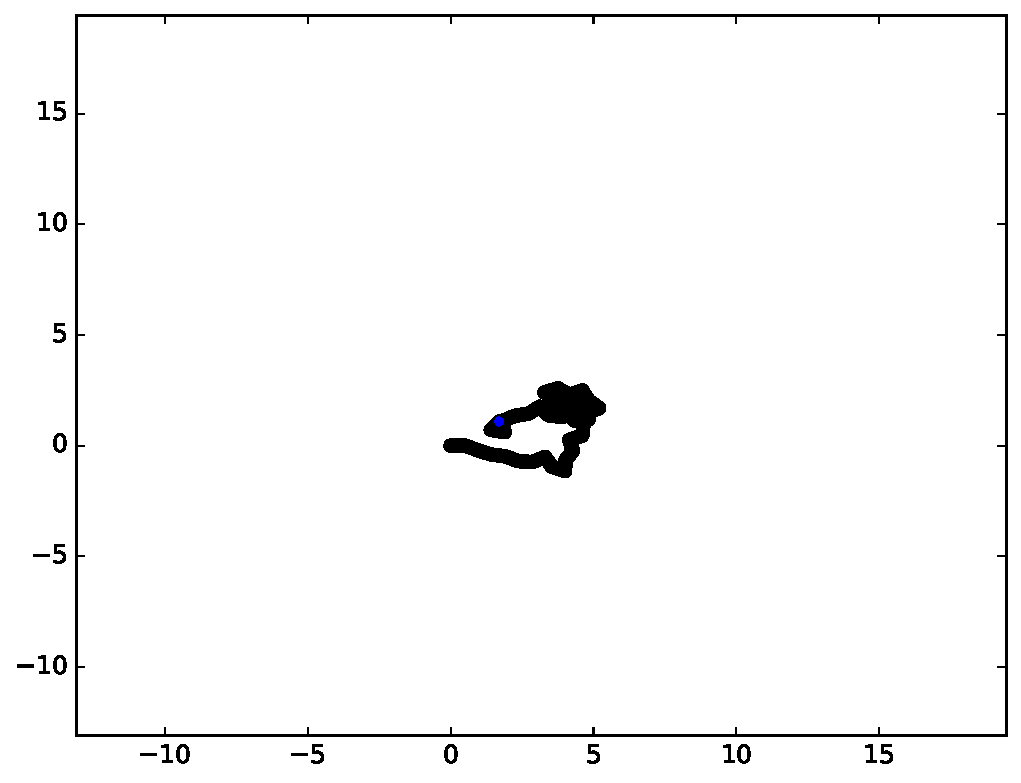
\includegraphics[width=\textwidth]{figures/ch3/spTraj_1_0_120_2}
			\caption[$S = 1$]{$S = 1$~cm/s.}
			\label{fig:spTraj_1_0_120_2}
		\end{subfigure}
		~
		\begin{subfigure}[t]{\subImgWmo}
			\centering
			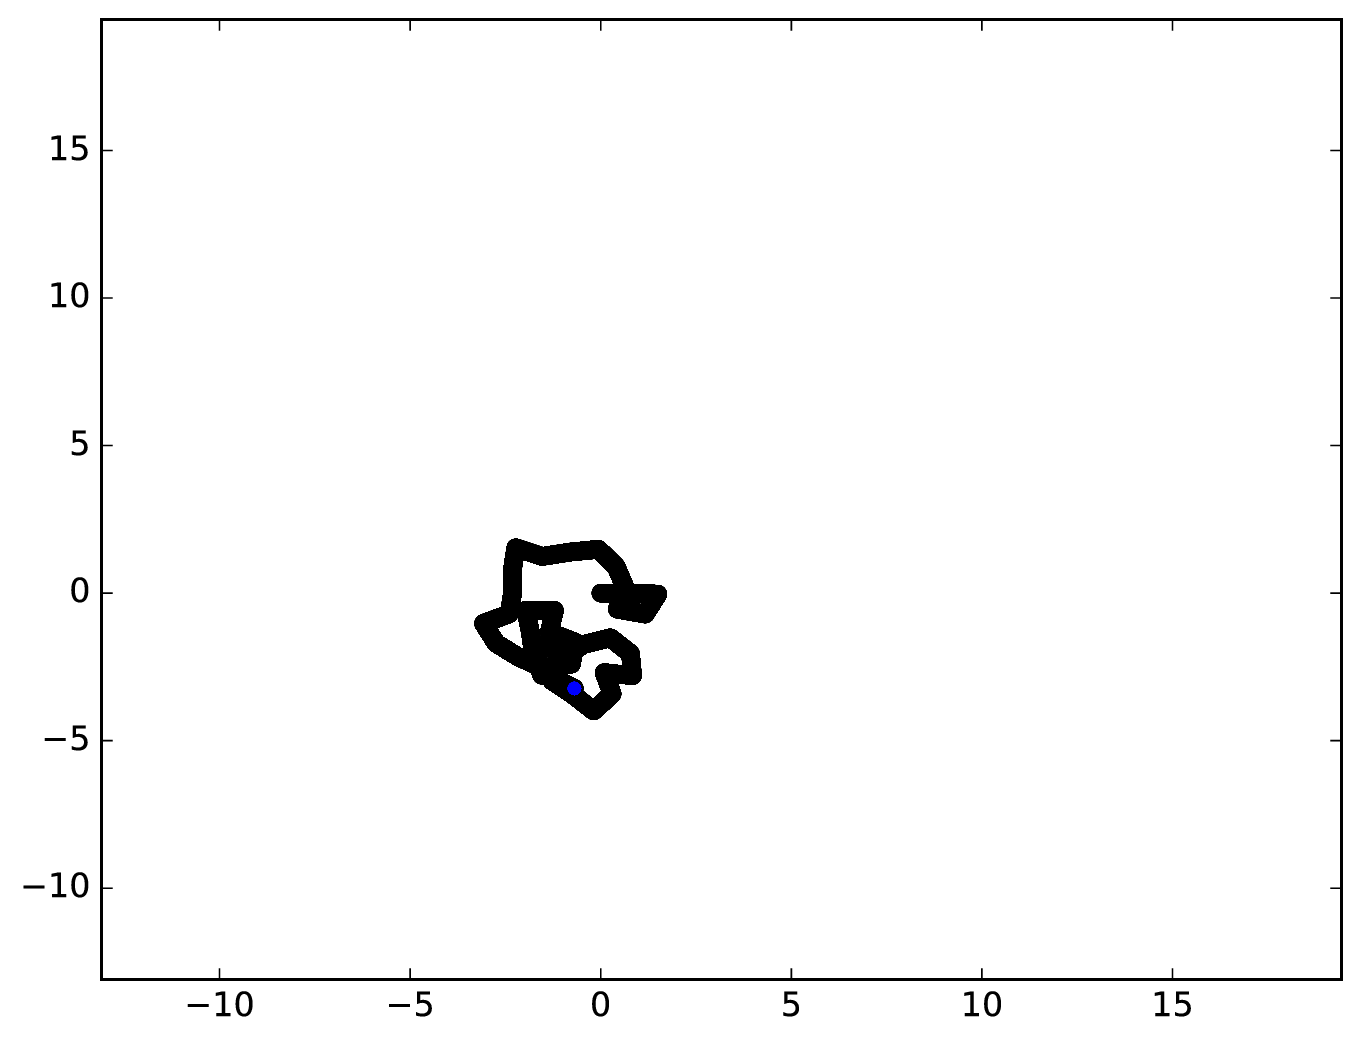
\includegraphics[width=\textwidth]{figures/ch3/spTraj_1_5_120_2}
			\caption[$S = 1,5$]{$S = 1,5$~cm/s.}
			\label{fig:spTraj_1_5_120_2}
		\end{subfigure}
		~
		\begin{subfigure}[t]{\subImgWmo}
			\centering
			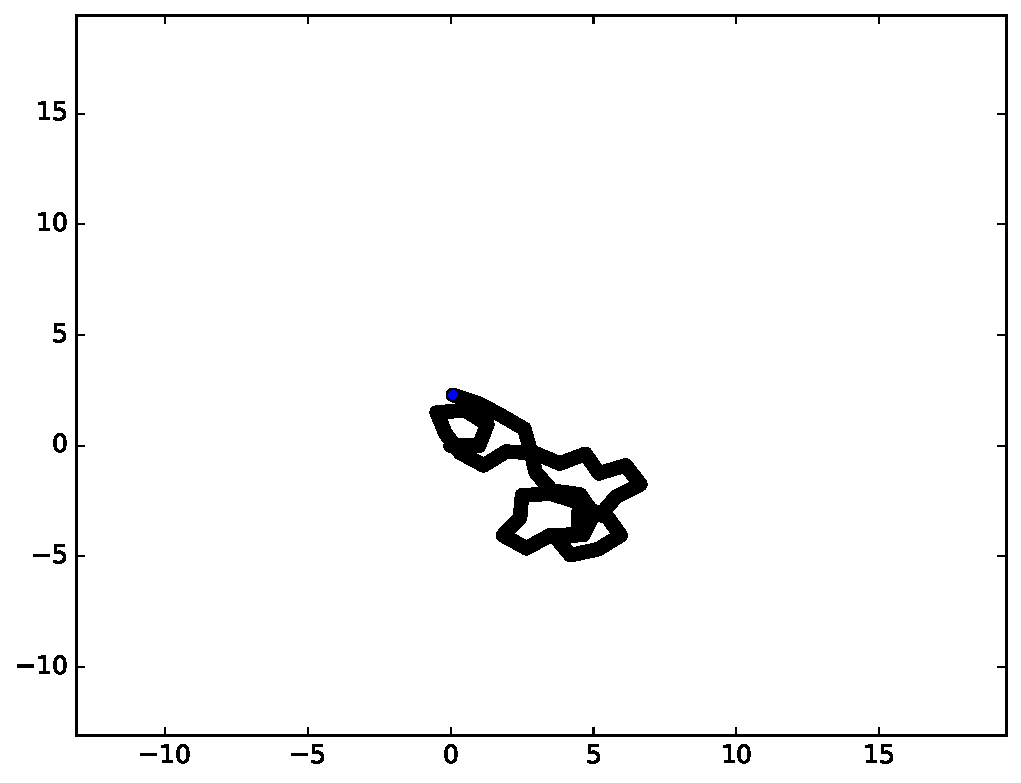
\includegraphics[width=\textwidth]{figures/ch3/spTraj_2_0_120_2}
			\caption[$S = 2,0$]{$S = 2,0$~cm/s.}
			\label{fig:spTraj_2_0_120_2}
		\end{subfigure}
		~
		\begin{subfigure}[t]{\subImgWmo}
			\centering
			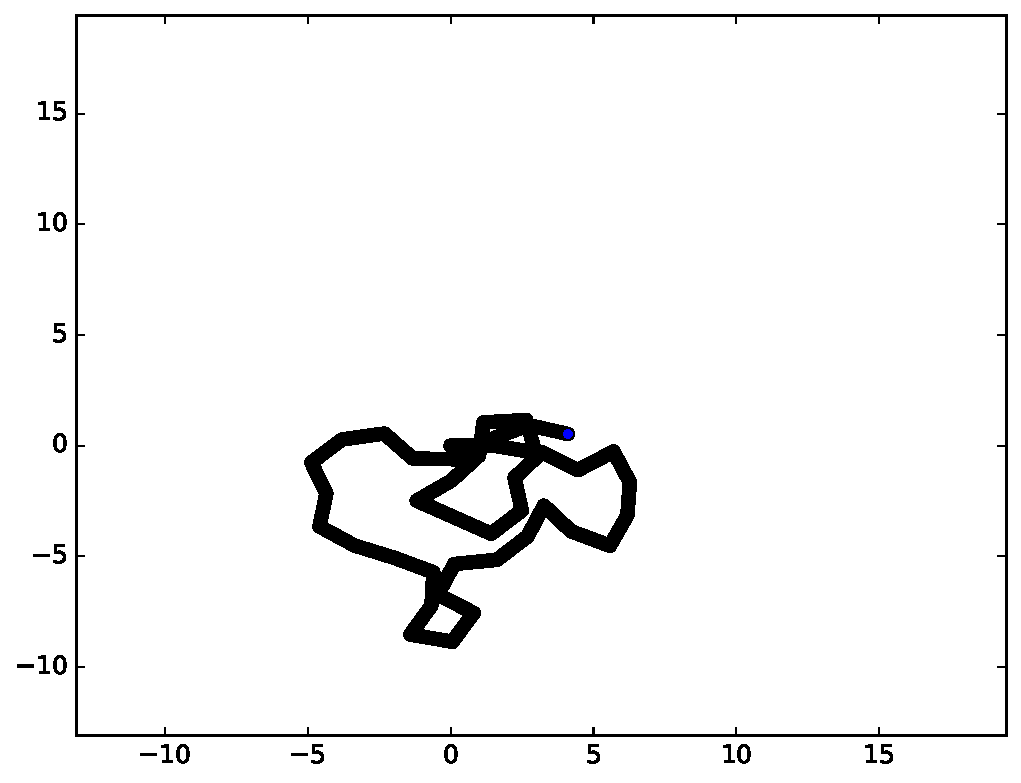
\includegraphics[width=\textwidth]{figures/ch3/spTraj_3_0_120_2}
			\caption[$S = 3,0$]{$S = 3,0$~cm/s.}
			\label{fig:spTraj_3_0_120_2}
		\end{subfigure}
		~
		\begin{subfigure}[t]{\subImgWmo}
			\centering
			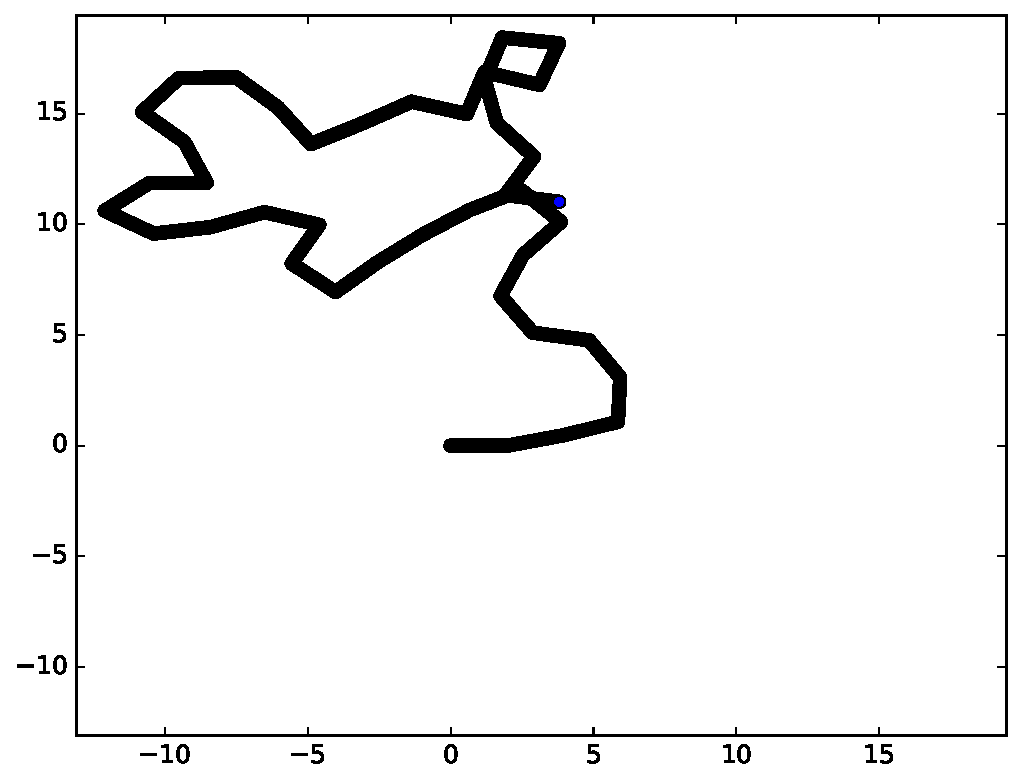
\includegraphics[width=\textwidth]{figures/ch3/spTraj_4_0_120_2}
			\caption[$S = 4,0$]{$S = 4,0$~cm/s.}
			\label{fig:spTraj_4_0_120_2}
		\end{subfigure}
		\caption[Effet des vitesses]{Trajectoires générées avec $A = 120\degree$ et $F = 2$~Hz, et des vitesses variables, de 0,5~cm/s à 4,0~cm/s. Pour mieux observer le phénomène de \og dilatation \fg{} des trajectoires, l'échelle est constante pour toutes les sous-figures.}
		\label{fig:spEffect}
	\end{figure}
	
	\subsubsection{Effet des angles}
	Lorsque $A$ est faible, comme sur la figure~\ref{fig:motion1530}, le mouvement est relativement lisse et régulier, avec des courbes rares et douces, sauf quand la valeur de $F$ augmente beaucoup ; et encore les trajectoires apparaissent-elles relativement \og dénouées \fg{}, à l'exception de celle de la figure~\ref{fig:synTraj_219_30_60} dont les valeurs de $A$ et $F$ commencent à être élevées, avec 30\textdegree{} et 60~Hz respectivement.
	
	À mesure que $A$ augmente, comme le montrera un examen successif des figures~\ref{fig:motion1530}, \ref{fig:motion4560}, \ref{fig:motion7590}, \ref{fig:motion105120}, \ref{fig:motion135150} et \ref{fig:motion165180}, les trajectoires sont de plus en plus irrégulières et \og nouées \fg{}.
	
	\subsubsection{Effet des fréquences}
	Un examen de n'importe quel bloc de six trajectoires pour une valeur de $A$ donnée montrera que plus $F$ est grand, plus les trajectoires sont irrégulières. Cet effet est très net et tout aussi visible quand $A$ est petit (comme sur la figure~\ref{fig:motion1530}) que quand il est grand (comme sur la figure~\ref{fig:motion165180}).
	
	Toutefois, quand $A$ est très grand, même avec une petite valeur de $F$, la trajectoire présente d'importantes irrégularités, comme sur la figure~\ref{fig:synTraj_219_180_1}. Notez cependant d'une part que ce n'est vrai que parce que nous observons la trajectoire sur une fenêtre temporelle relativement longue (20 secondes) et d'autre part que nous aurions pu choisir une valeur de $F$ bien plus faible, comme 0,1~Hz, par exemple, voire moins. Si $F$ était strictement inférieure à 0,05~Hz, sur une fenêtre de 20 secondes, la trajectoire serait rectiligne.
	
	\subsubsection{Effet combiné des angles et fréquences}
	L'effet des fréquences étant qualitativement comparable à celui des angles, on peut considérer que ces paramètres sont approximativement équivalents et, de fait, les regrouper en un seul par un produit. Ainsi, l'on peut s'intéresser non pas à leurs valeurs respectives mais au produit $AF$, que nous avons également baptisé \emph{pseudo-entropie}.
	
	Insistons sur le fait qu'il s'agit d'une approximation, mais notez que pour une valeur de $AF$ de 480, par exemple, on a les trajectoires de la figure~\ref{fig:synTraj_219_30_16} et celle de la figure~\ref{fig:synTraj_219_120_4}. Bien que visiblement distinctes, ces deux trajectoires présentent un niveau d'irrégularité grossièrement comparable. Pour $AF = 720$, les trajectoires des figures~\ref{fig:synTraj_219_90_8} et~\ref{fig:synTraj_219_45_16} sont également assez semblables.
	
	Notons tout de même que pour une valeur de $AF$ donnée, même si l'irrégularité globale est généralement comparable, une trajectoire générée par une valeur de $F$ relativement élevée tend à être plus lisse et courbée, tandis que quand $A$ domine, elle est plutôt \og saccadée \fg{}.
	
	Ce point sera particulièrement visible avec la même valeur de $AF$ de 180, mais en comparant les trajectoires présentées sur la figure~\ref{fig:trajsAF180}. En effet, si $180 \times 1 = 15 \times 12 = 180$, nous avons dans un cas un $A$ très grand avec un $F$ très petit, et dans l'autre des valeurs plus \og équilibrées \fg{}. Le résultat est une trajectoire très saccadée sur la première trajectoire (figure~\ref{fig:synTraj_219_180_1b}) et plutôt lisse et courbe sur la seconde (figure~\ref{fig:synTraj_219_15_12}).
	
	\begin{figure}[htb]
		\begin{subfigure}[t]{0.49\textwidth}
			\centering
			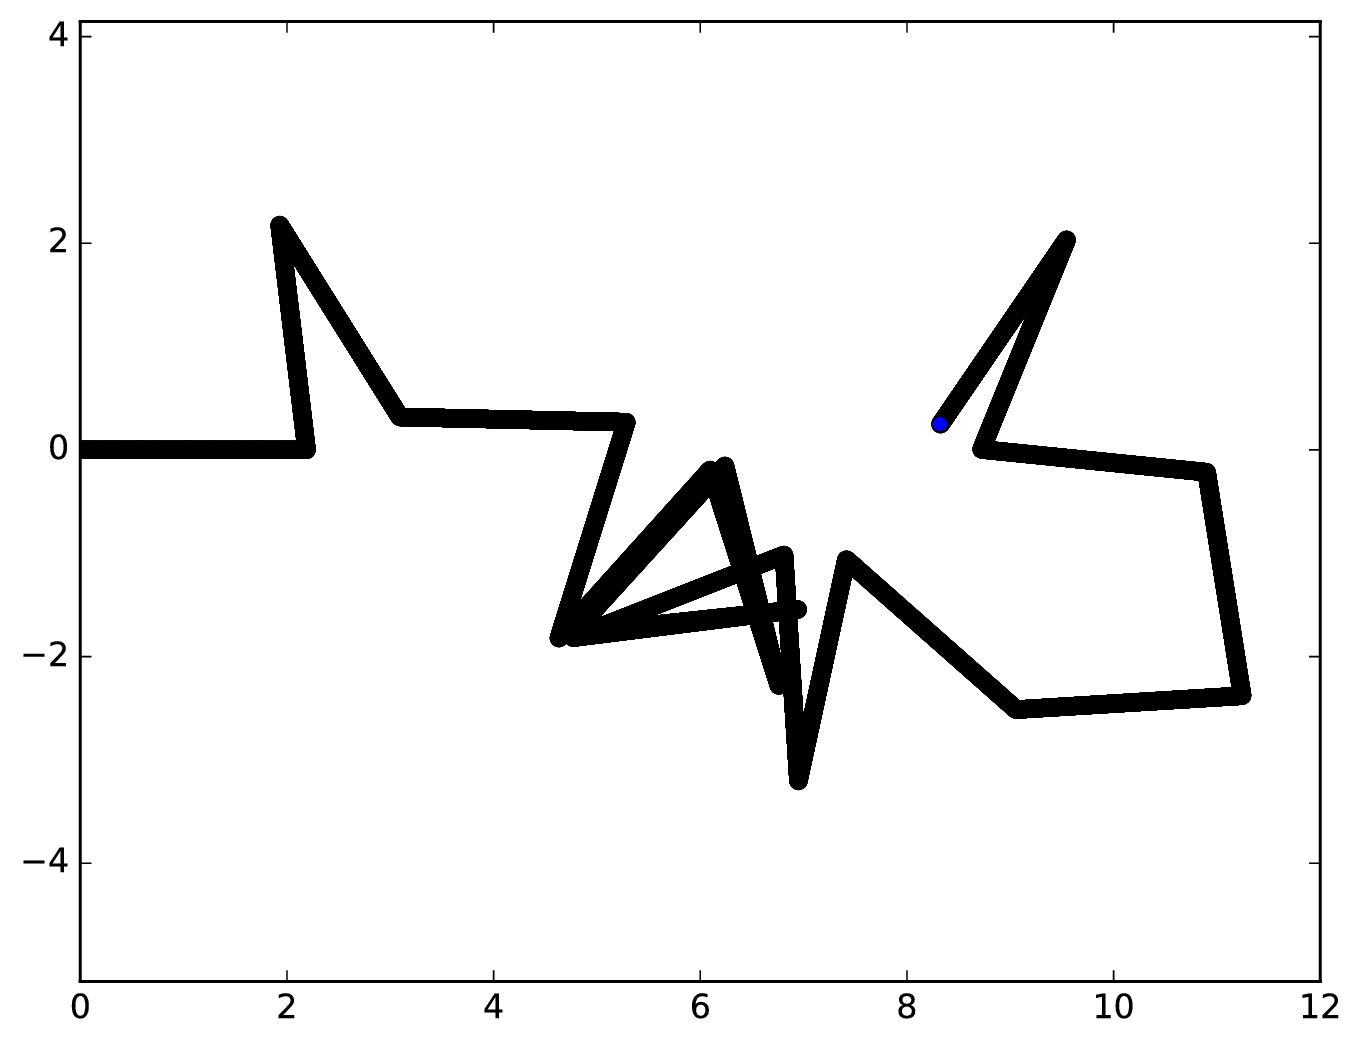
\includegraphics[width=\textwidth]{figures/ch3/synTraj_219_180_1}
			\caption[$A = 180$, $F=1$]{$A = 180$, $F=1$}
			\label{fig:synTraj_219_180_1b}
		\end{subfigure}
		~
		\begin{subfigure}[t]{0.49\textwidth}
			\centering
			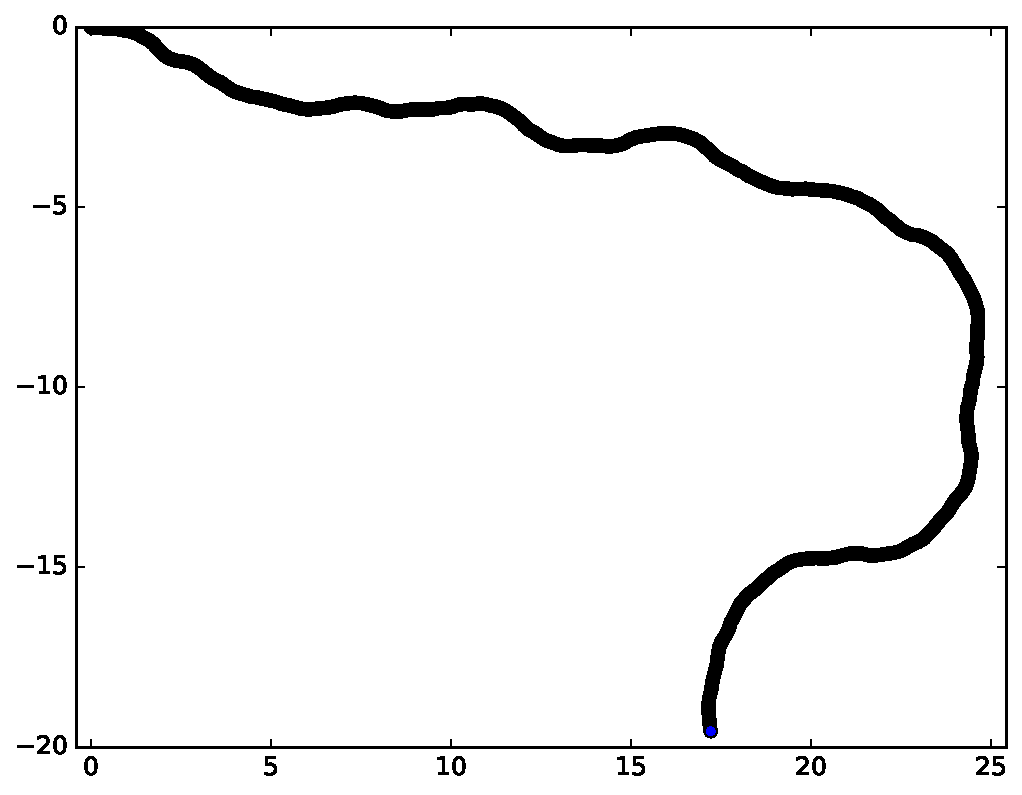
\includegraphics[width=\textwidth]{figures/ch3/synTraj_219_15_12}
			\caption[$A = 15$, $F=12$]{$A = 15$, $F=12$}
			\label{fig:synTraj_219_15_12}
		\end{subfigure}
		\caption[Trajectoires pour $AF = 180$]{Trajectoires pour $AF = 180$ et $S = 2,19~cm/s$. On observe que pour un produit $AF$ donné, si $A$ est particulièrement grand et $F$ particulièrement petit sur une trajectoire (et inversement sur l'autre) les résultats obtenus diffèrent significativement.}
		\label{fig:trajsAF180}
	\end{figure}
	
	
	L'on pourra donc, dans certains cas, utiliser le produit $AF$ seul, pour simplifier l'étude des résultats, mais il convient de le faire en ayant à l'esprit que c'est une approximation, et qu'elle tend à être moins précise pour les valeurs de $A$ ou $F$ particulièrement faibles ou élevées.
	
	\subsubsection{Longueur des trajectoires, périmètres des enveloppes convexes}
	Pour rappel, toutes les trajectoires des figures~\ref{fig:motion1530}, \ref{fig:motion4560}, \ref{fig:motion7590}, \ref{fig:motion105120}, \ref{fig:motion135150} et \ref{fig:motion165180} furent générées par un mouvement de vitesse constante, 2,19~cm/s. Attendu qu'elles ont également été générées sur une même durée (20 secondes) elles ont toutes la même longueur, malgré les apparences dues aux variations d'échelle : $2,19~cm/s \times 20~s = 43,8~cm$.
	
	Mais certaines trajectoires sont très peu \og nouées \fg{} tandis que d'autres le sont beaucoup. De fait, l'espace horizontal ou vertical qu'elles occupent peut varier considérablement. Par exemple, comme nous le mentionnions plus haut, la trajectoire de la figure~\ref{fig:synTraj_219_15_1} parcourt plus de 40~cm à l'horizontale, tandis que celle de la figure~\ref{fig:synTraj_219_180_60} est contenue dans un rectangle d'environ 1,2~cm de hauteur sur 1~cm de largeur.
	
	En règle générale, plus la pseudo-entropie est faible, plus la trajectoire parcourra une distance horizontale ou verticale importante, et plus la pseudo-entropie est élevée, plus ces distances sont faibles. Notez cependant que cela n'implique pas nécessairement qu'une trajectoire de faible pseudo-entropie occupera forcément une aire importante, car comme le montre la figure~\ref{fig:synTraj_219_30_1}, la distance parcourue sur un axe (vertical, en l'occurrence) peut être très faible.
	
	\begin{figure}[htb]
		\begin{subfigure}[t]{\subImgWmo}
			\centering
			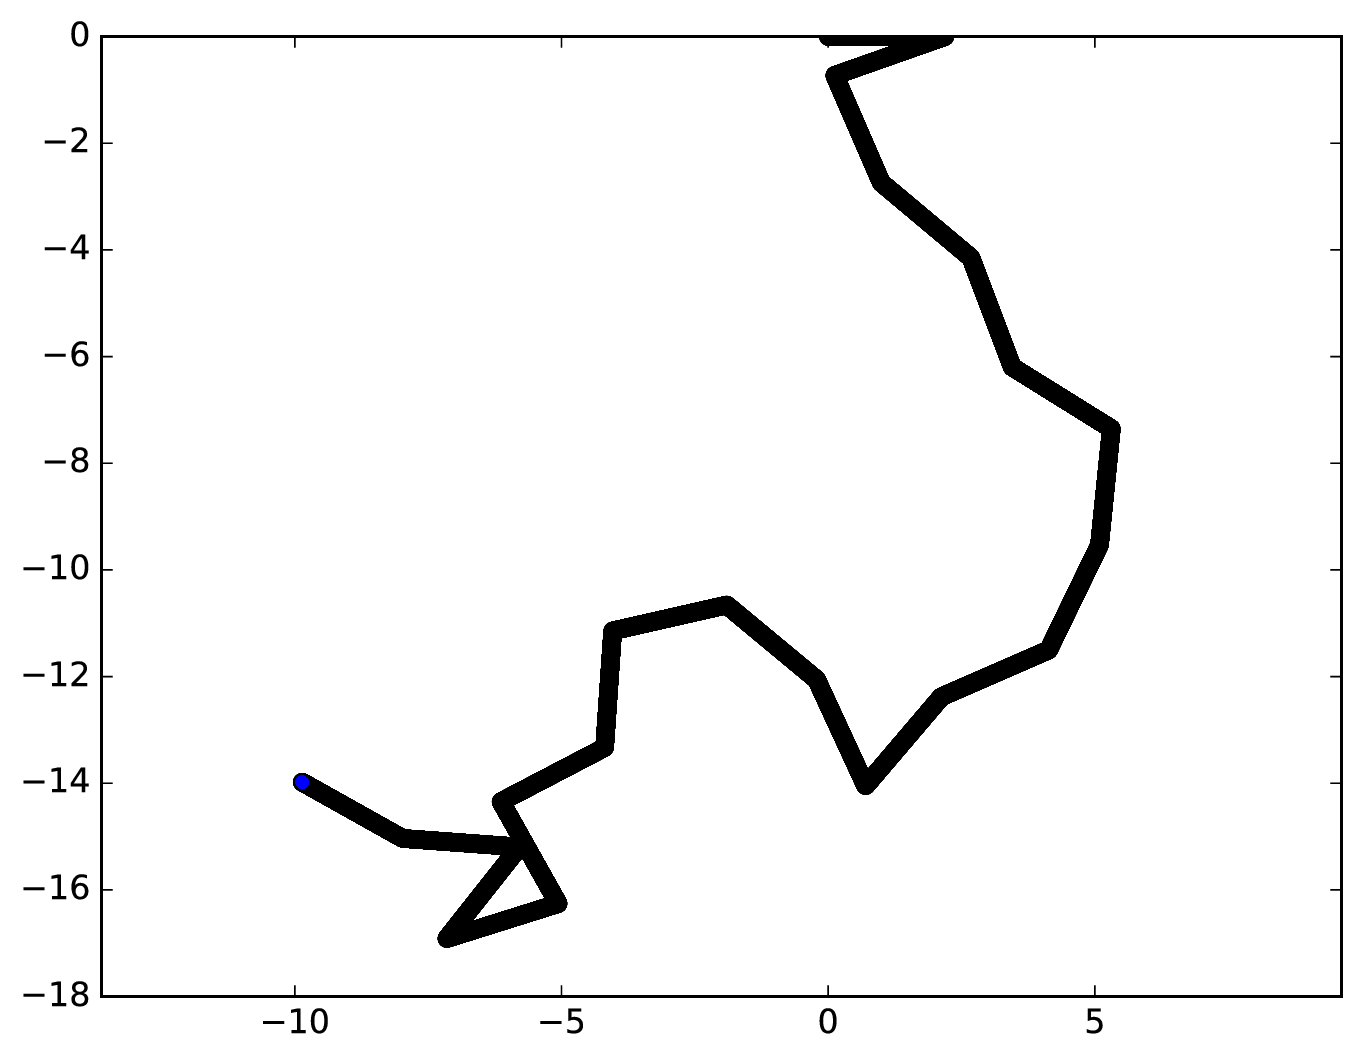
\includegraphics[width=\textwidth]{figures/ch3/synTraj_219_165_1}
			\caption[$A = 165$, $F=1$]{$A = 165$, $F=1$}
			\label{fig:synTraj_219_165_1}
		\end{subfigure}
		~
		\begin{subfigure}[t]{\subImgWmo}
			\centering
			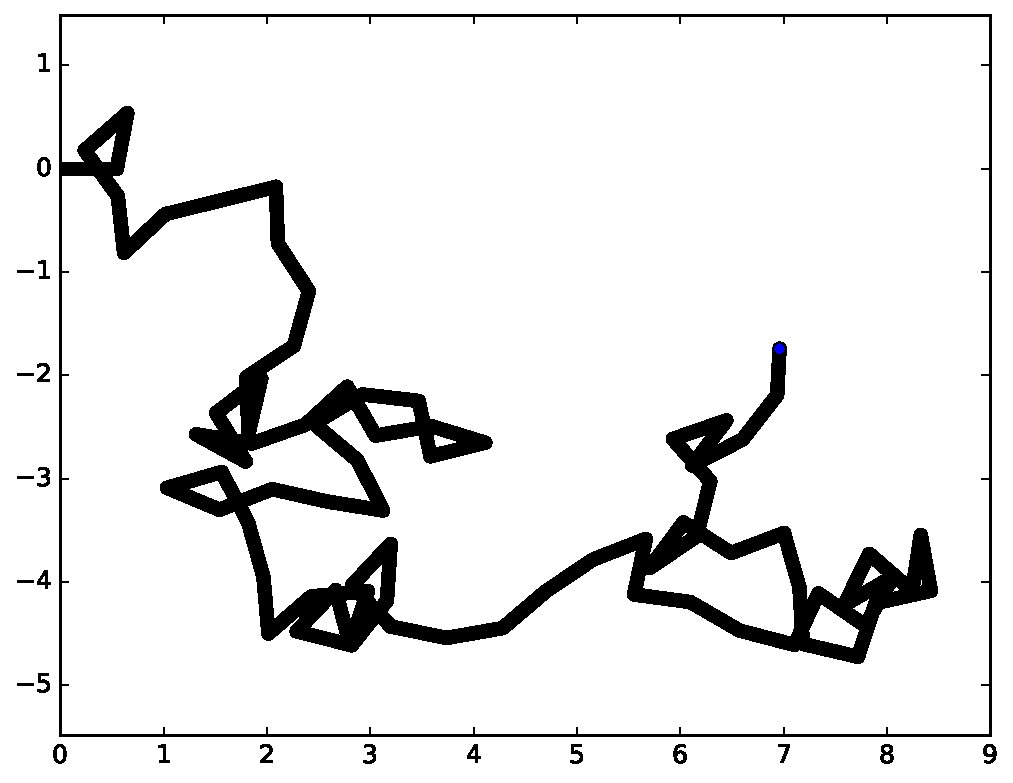
\includegraphics[width=\textwidth]{figures/ch3/synTraj_219_165_4}
			\caption[$A = 165$, $F=4$]{$A = 165$, $F=4$}
			\label{fig:synTraj_219_165_4}
		\end{subfigure}
		~
		\begin{subfigure}[t]{\subImgWmo}
			\centering
			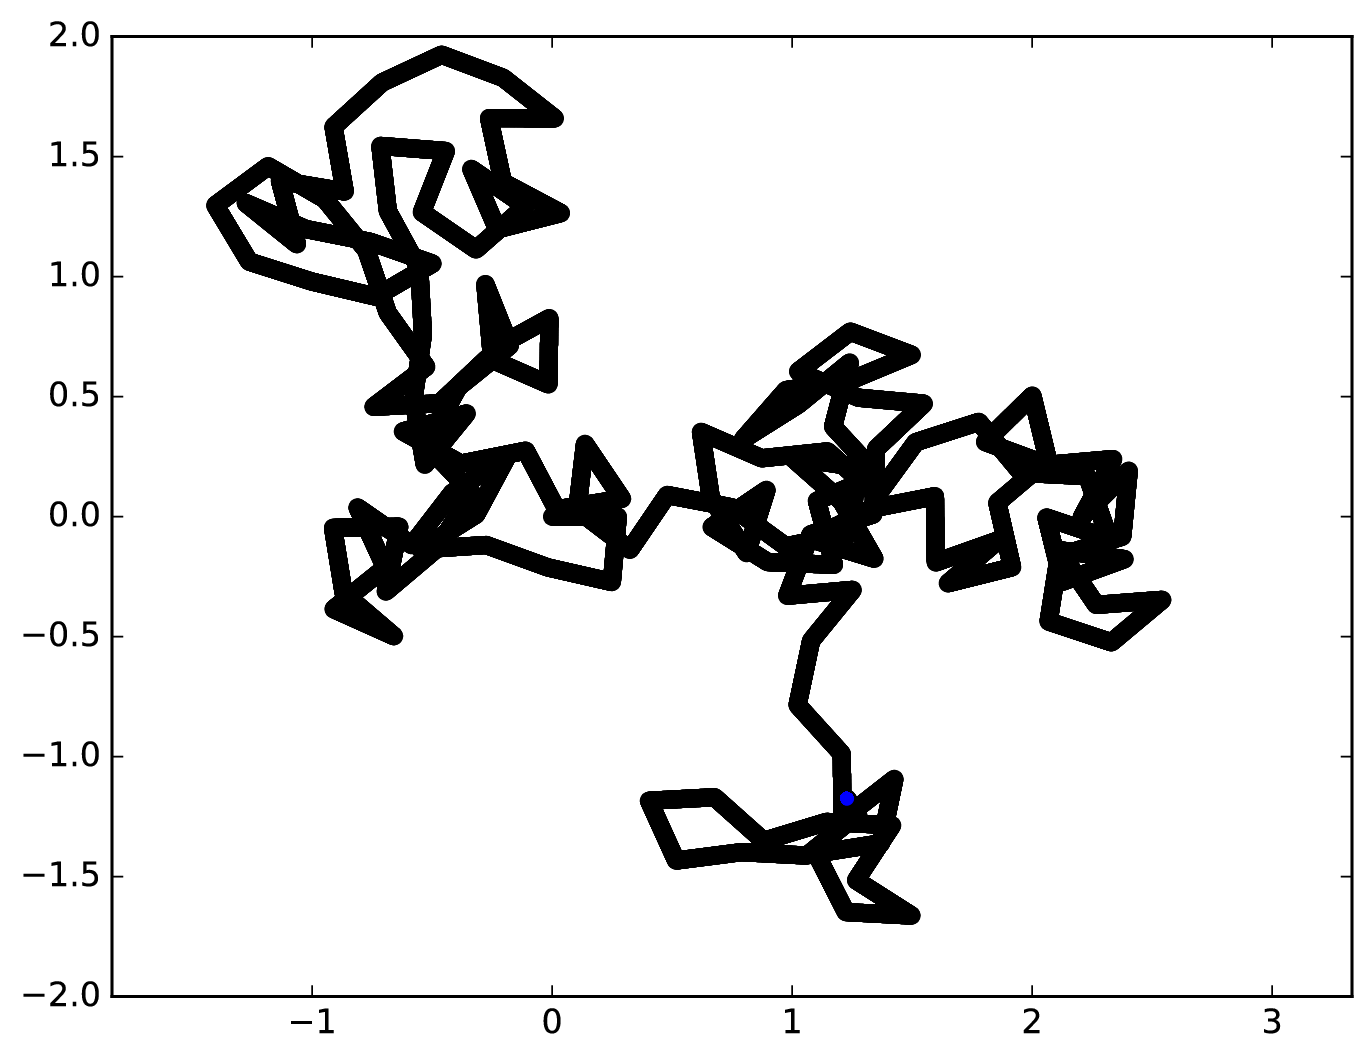
\includegraphics[width=\textwidth]{figures/ch3/synTraj_219_165_8}
			\caption[$A = 165$, $F=8$]{$A = 165$, $F=8$}
			\label{fig:synTraj_219_165_8}
		\end{subfigure}
		~
		\begin{subfigure}[t]{\subImgWmo}
			\centering
			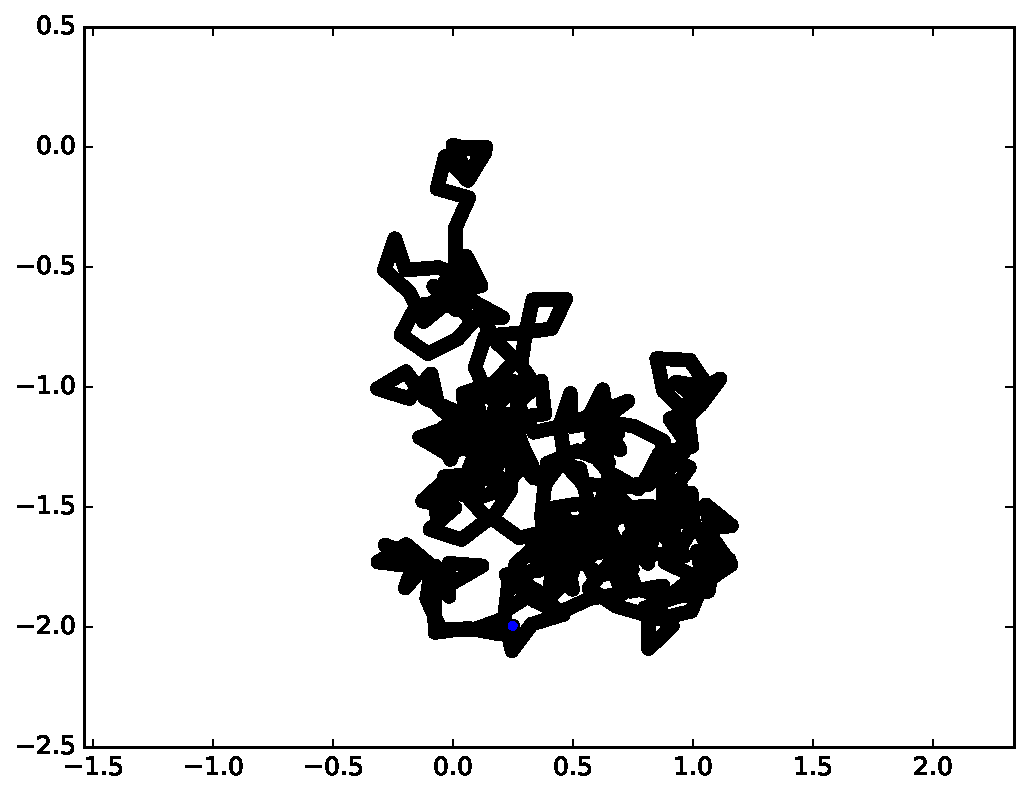
\includegraphics[width=\textwidth]{figures/ch3/synTraj_219_165_16}
			\caption[$A = 165$, $F=16$]{$A = 165$, $F=16$}
			\label{fig:synTraj_219_165_16}
		\end{subfigure}
		~
		\begin{subfigure}[t]{\subImgWmo}
			\centering
			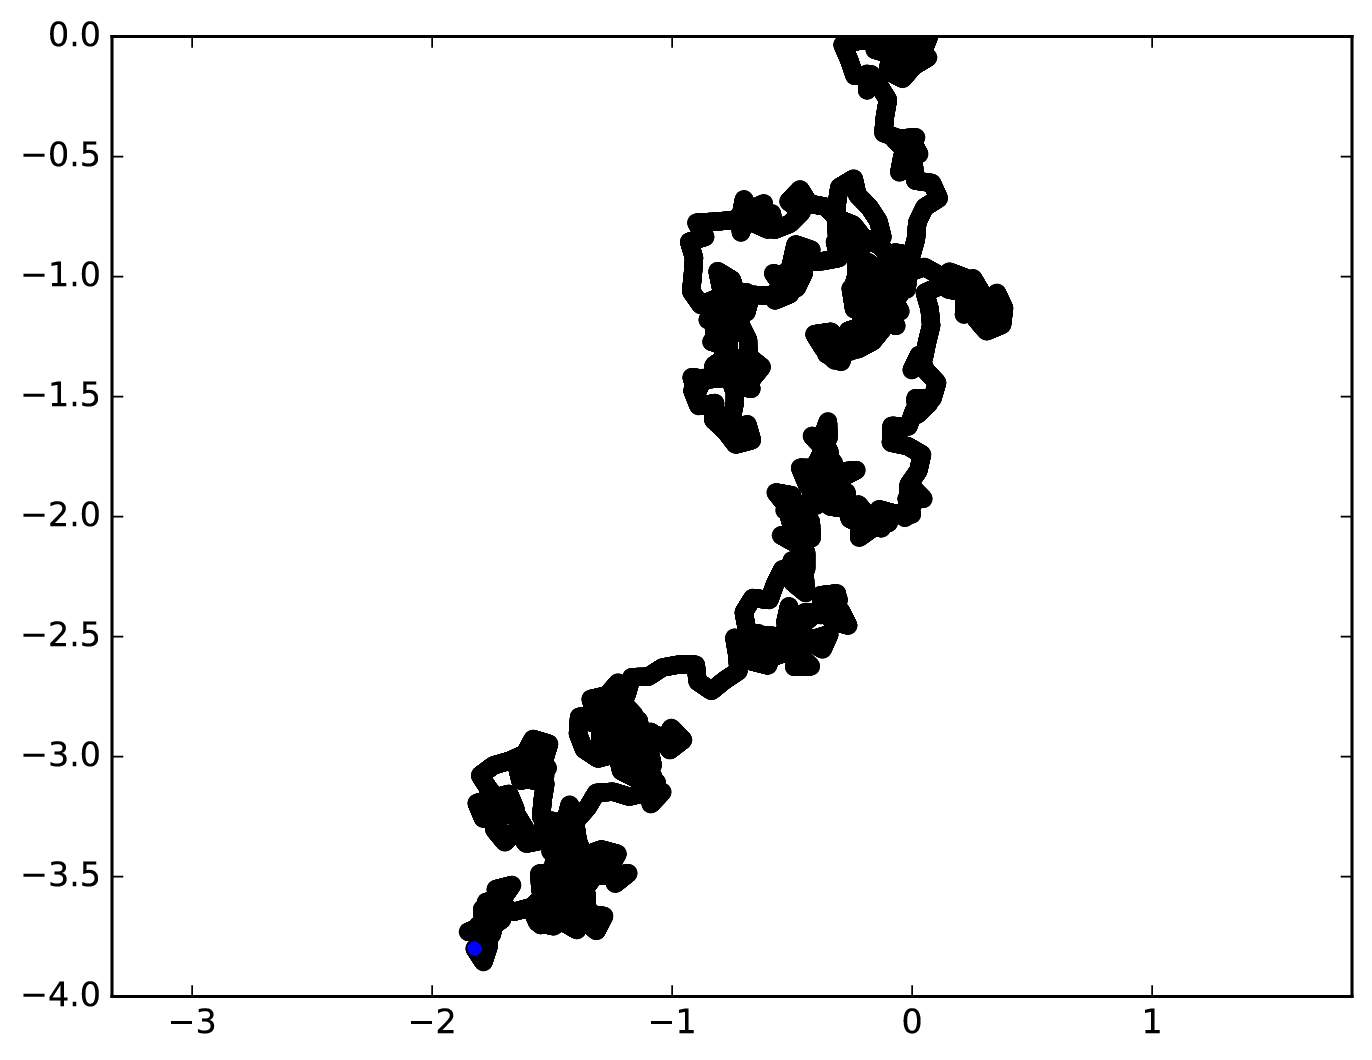
\includegraphics[width=\textwidth]{figures/ch3/synTraj_219_165_32}
			\caption[$A = 165$, $F=32$]{$A = 165$, $F=32$}
			\label{fig:synTraj_219_165_32}
		\end{subfigure}
		~
		\begin{subfigure}[t]{\subImgWmo}
			\centering
			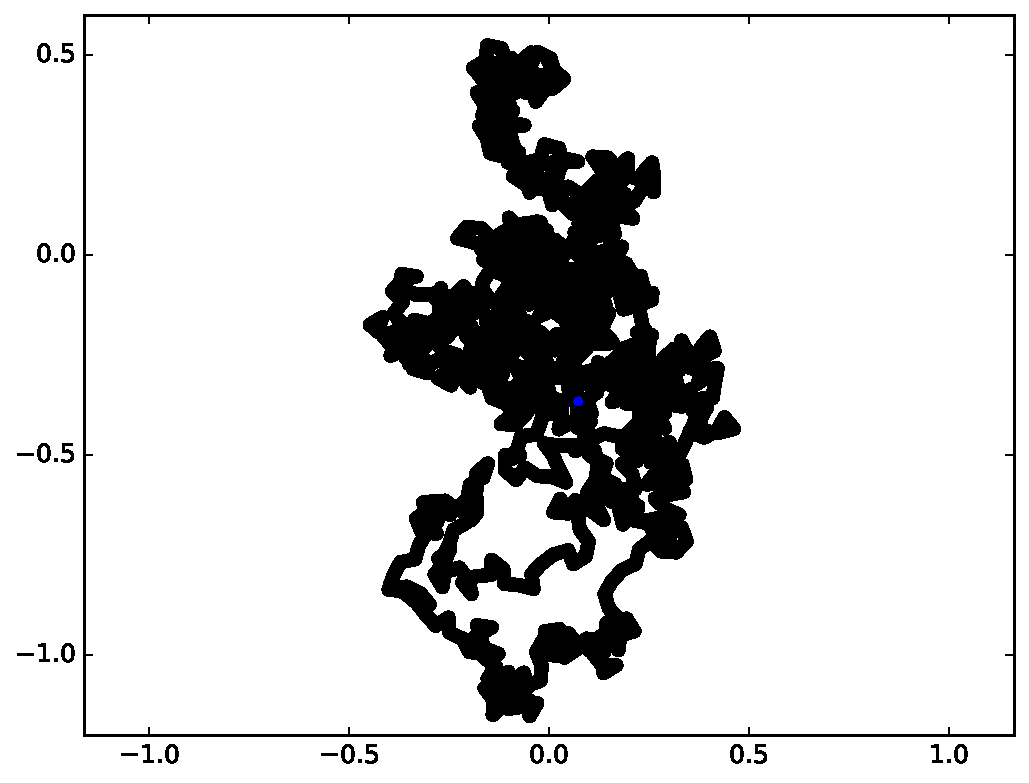
\includegraphics[width=\textwidth]{figures/ch3/synTraj_219_165_60}
			\caption[$A = 165$, $F=60$]{$A = 165$, $F=60$}
			\label{fig:synTraj_219_165_60}
		\end{subfigure}
		~
		\begin{subfigure}[t]{\subImgWmo}
			\centering
			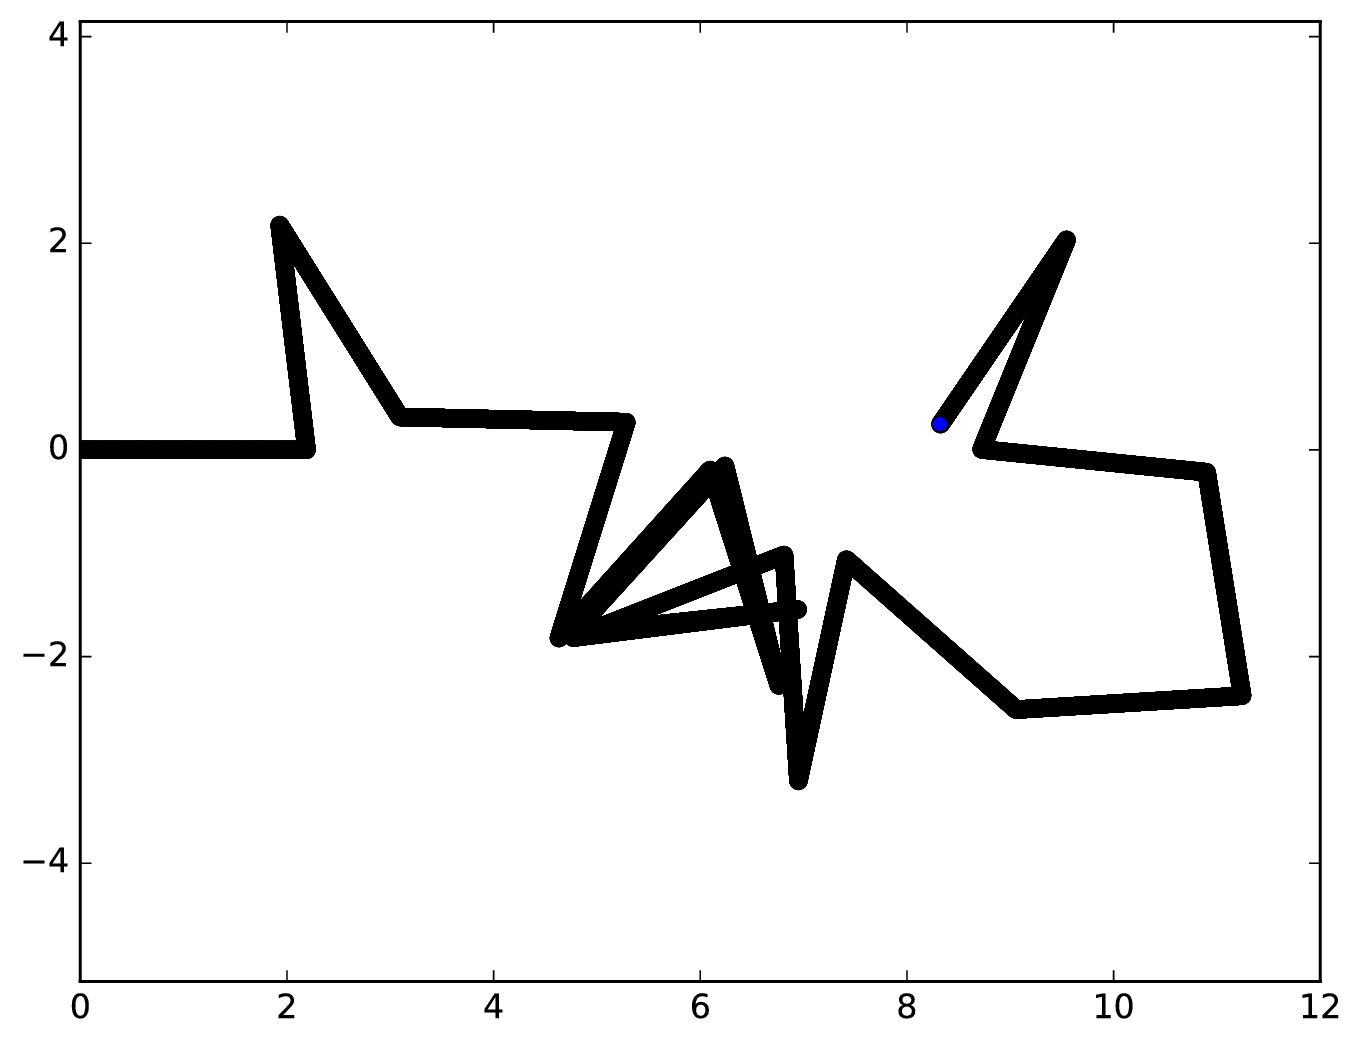
\includegraphics[width=\textwidth]{figures/ch3/synTraj_219_180_1}
			\caption[$A = 180$, $F=1$]{$A = 180$, $F=1$}
			\label{fig:synTraj_219_180_1}
		\end{subfigure}
		~
		\begin{subfigure}[t]{\subImgWmo}
			\centering
			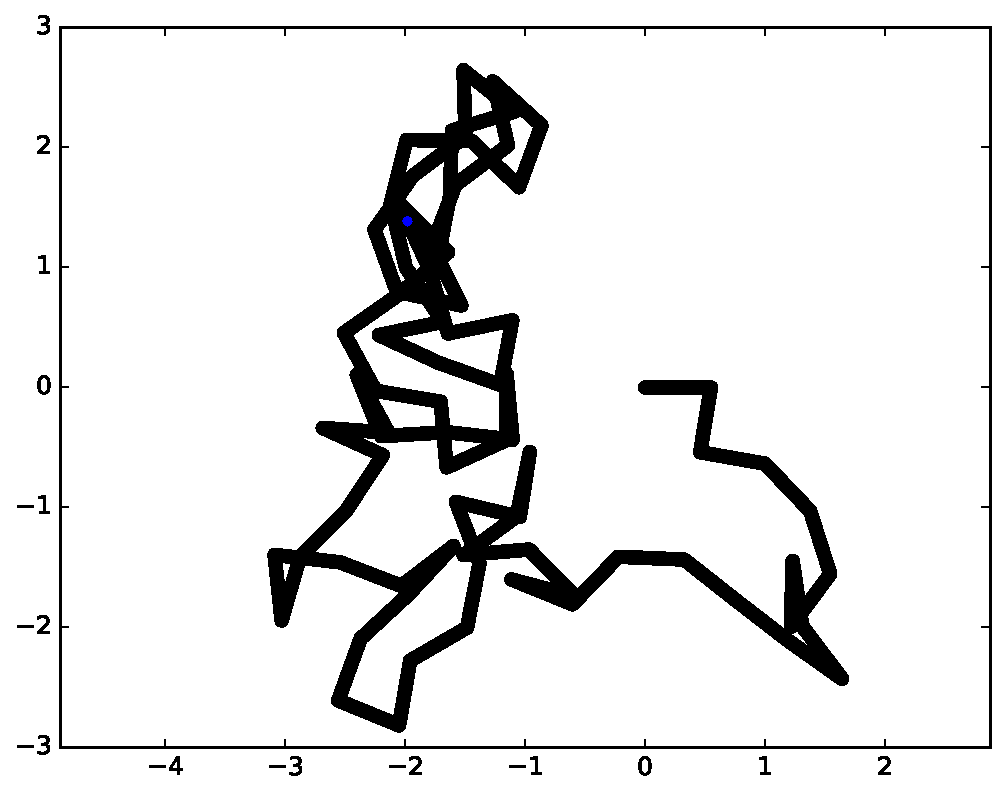
\includegraphics[width=\textwidth]{figures/ch3/synTraj_219_180_4}
			\caption[$A = 180$, $F=4$]{$A = 180$, $F=4$}
			\label{fig:synTraj_219_180_4}
		\end{subfigure}
		~
		\begin{subfigure}[t]{\subImgWmo}
			\centering
			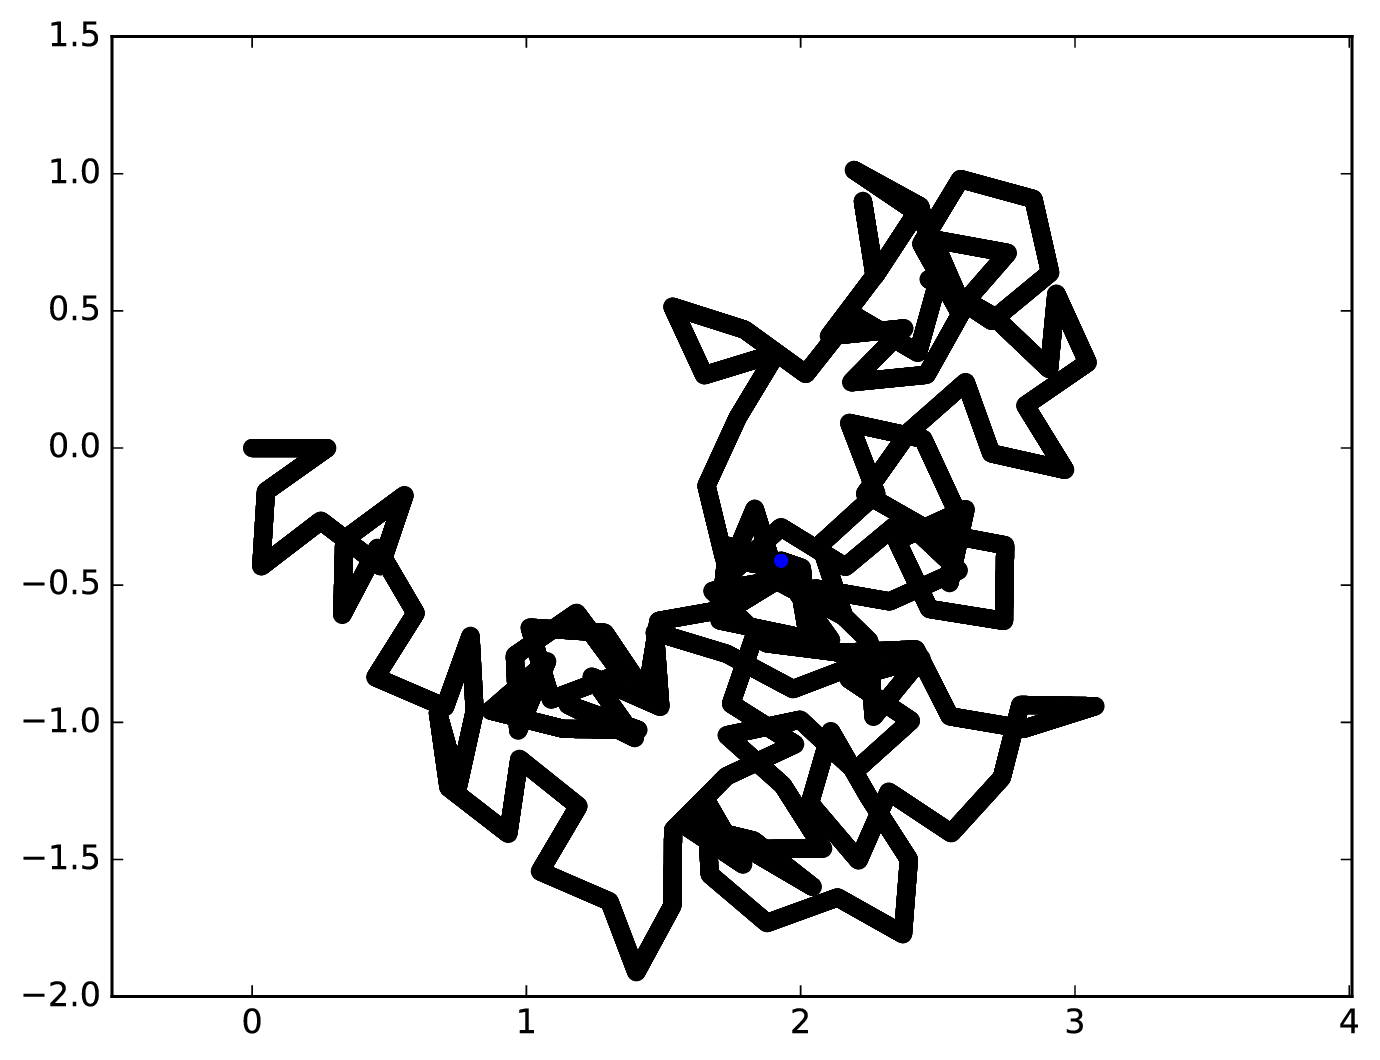
\includegraphics[width=\textwidth]{figures/ch3/synTraj_219_180_8}
			\caption[$A = 180$, $F=1$]{$A = 180$, $F=8$}
			\label{fig:synTraj_219_180_8}
		\end{subfigure}
		~
		\begin{subfigure}[t]{\subImgWmo}
			\centering
			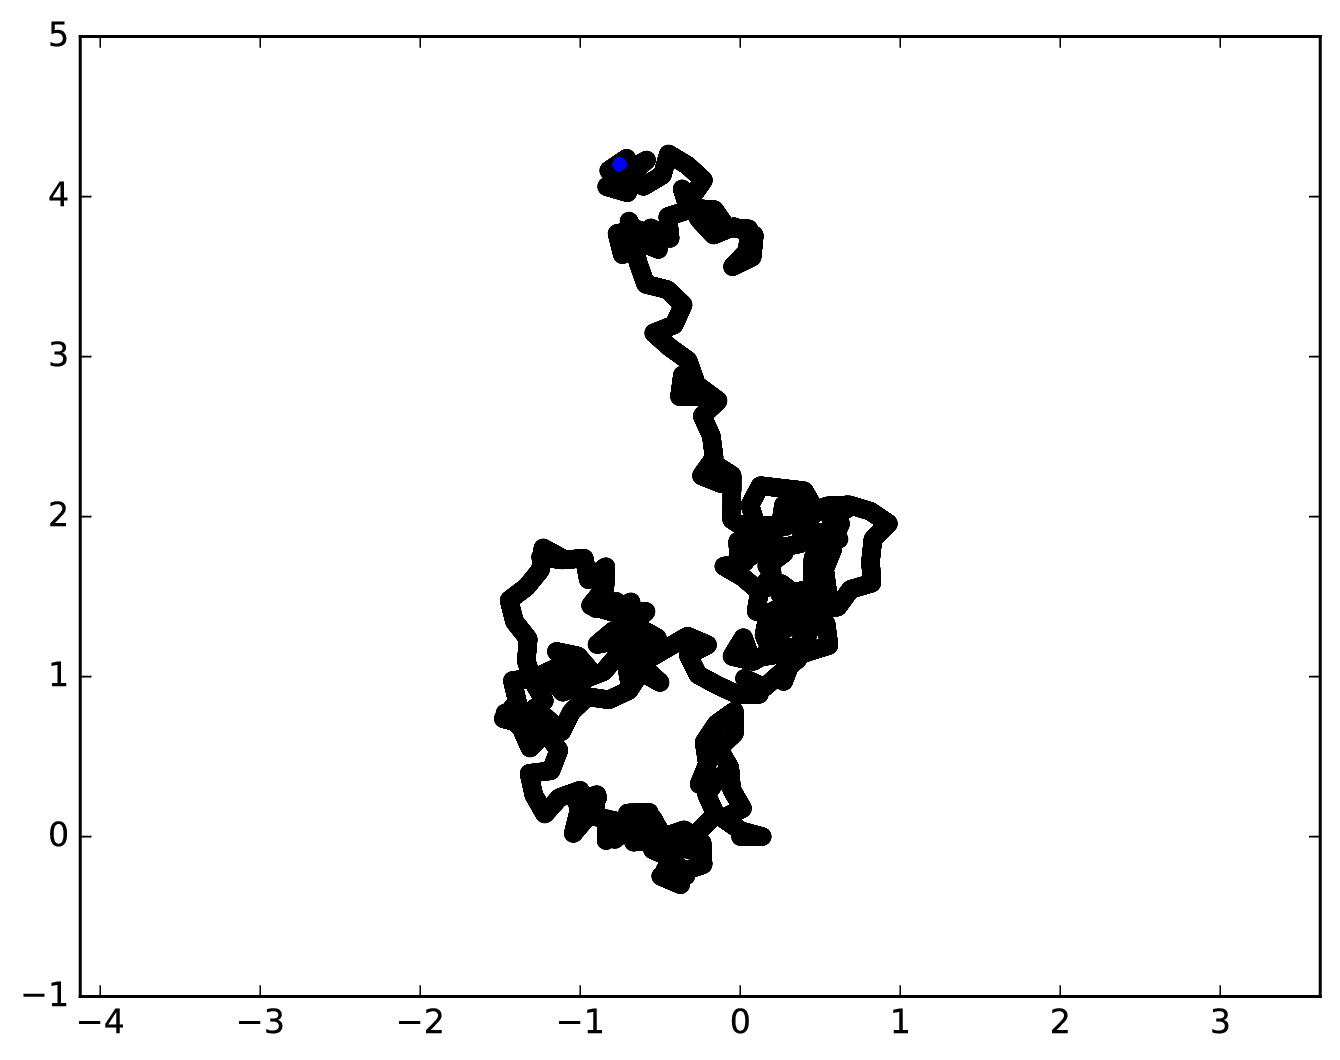
\includegraphics[width=\textwidth]{figures/ch3/synTraj_219_180_16}
			\caption[$A = 180$, $F=16$]{$A = 180$, $F=16$}
			\label{fig:synTraj_219_180_16}
		\end{subfigure}
		~
		\begin{subfigure}[t]{\subImgWmo}
			\centering
			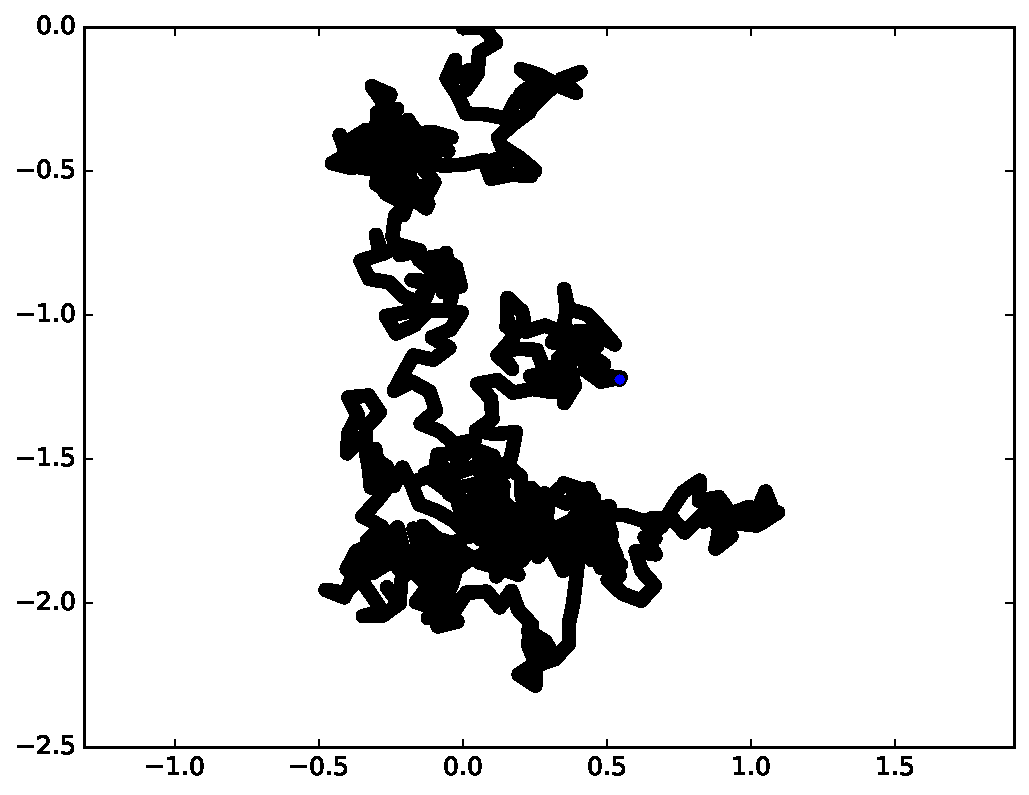
\includegraphics[width=\textwidth]{figures/ch3/synTraj_219_180_32}
			\caption[$A = 180$, $F=32$]{$A = 180$, $F=32$}
			\label{fig:synTraj_219_180_32}
		\end{subfigure}
		~
		\begin{subfigure}[t]{\subImgWmo}
			\centering
			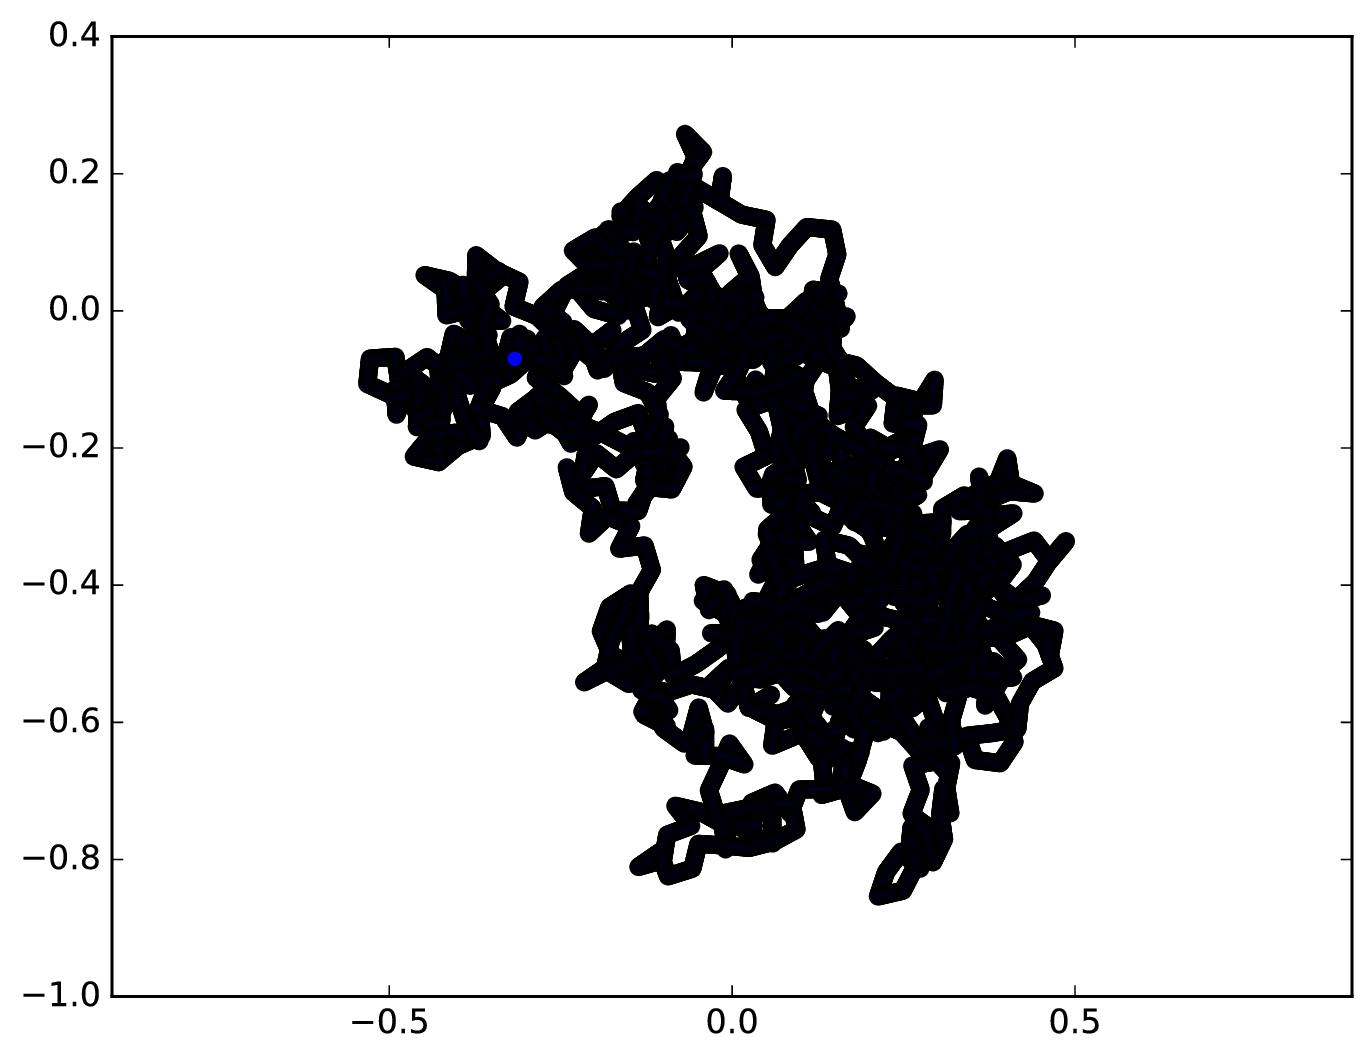
\includegraphics[width=\textwidth]{figures/ch3/synTraj_219_180_60}
			\caption[$A = 180$, $F=60$]{$A = 180$, $F=60$}
			\label{fig:synTraj_219_180_60}
		\end{subfigure}
		\caption[Mouvements générés par notre modèle -- VI]{Exemples de trajectoires générées par notre modèle pour un objet de vitesse constante (2,19~cm/s).}
		\label{fig:motion165180}
	\end{figure}
	
	Une façon d'estimer la surface occupée par un ensemble de points (comme une trajectoire) consiste déterminer son enveloppe convexe. L'enveloppe convexe d'un ensemble de points du plan est le plus petit polygone convexe contenant tous les points de l'ensemble. Dans un espace en trois dimensions, l'enveloppe convexe est, de façon analogue, le plus petit polyèdre convexe contenant tous les points de l'ensemble. Des exemples d'enveloppes convexes sont représentés sur la figure~\ref{fig:trajAreas}. On y remarque notamment une relation inverse entre la pseudo-entropie et le périmètre de l'enveloppe convexe de la trajectoire. Les trajectoires de pseudo-entropie très faible, telle que celle de la figure~\ref{fig:areaTraj_2_19_1_16}, occupent un espace important, tandis que les trajectoires de très forte pseudo-entropie, comme celle de la figure~\ref{fig:areaTraj_2_19_180_240}, sont confinées à une toute petite zone.
	
	
	\begin{figure}[htb]
		\centering
		\begin{subfigure}[t]{\subImgWmo}
			\centering
			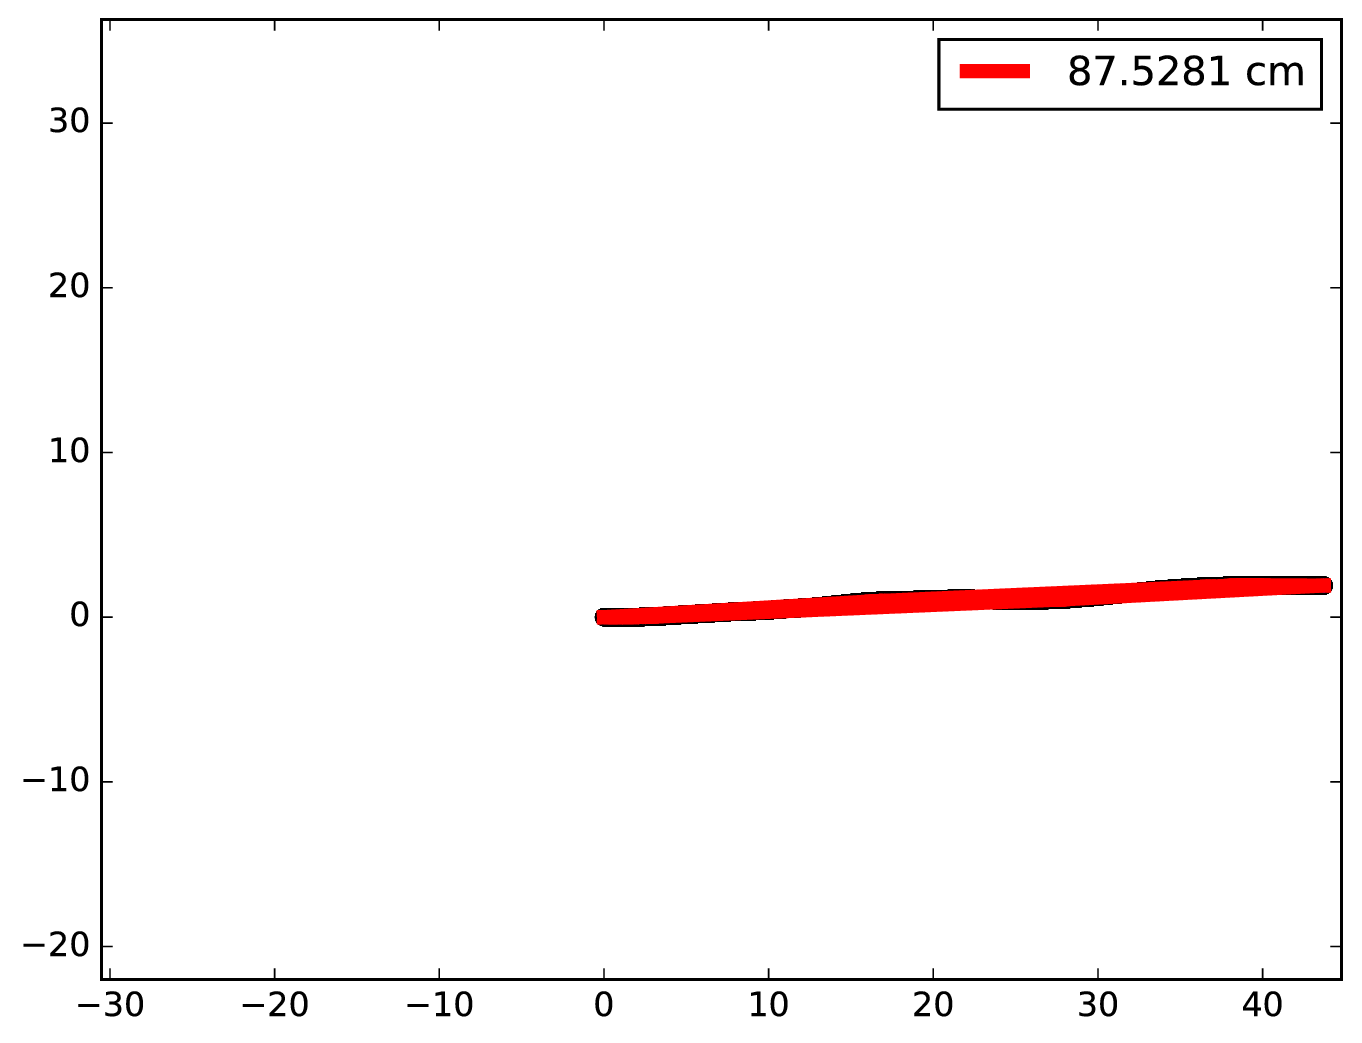
\includegraphics[width=\textwidth]{figures/ch3/areaTraj_2_19_1_16}
			\caption{$A = 1$, $F=16$, $AF=16$. $P\approx~87$~cm.}
			\label{fig:areaTraj_2_19_1_16}
		\end{subfigure}
		~
		\begin{subfigure}[t]{\subImgWmo}
			\centering
			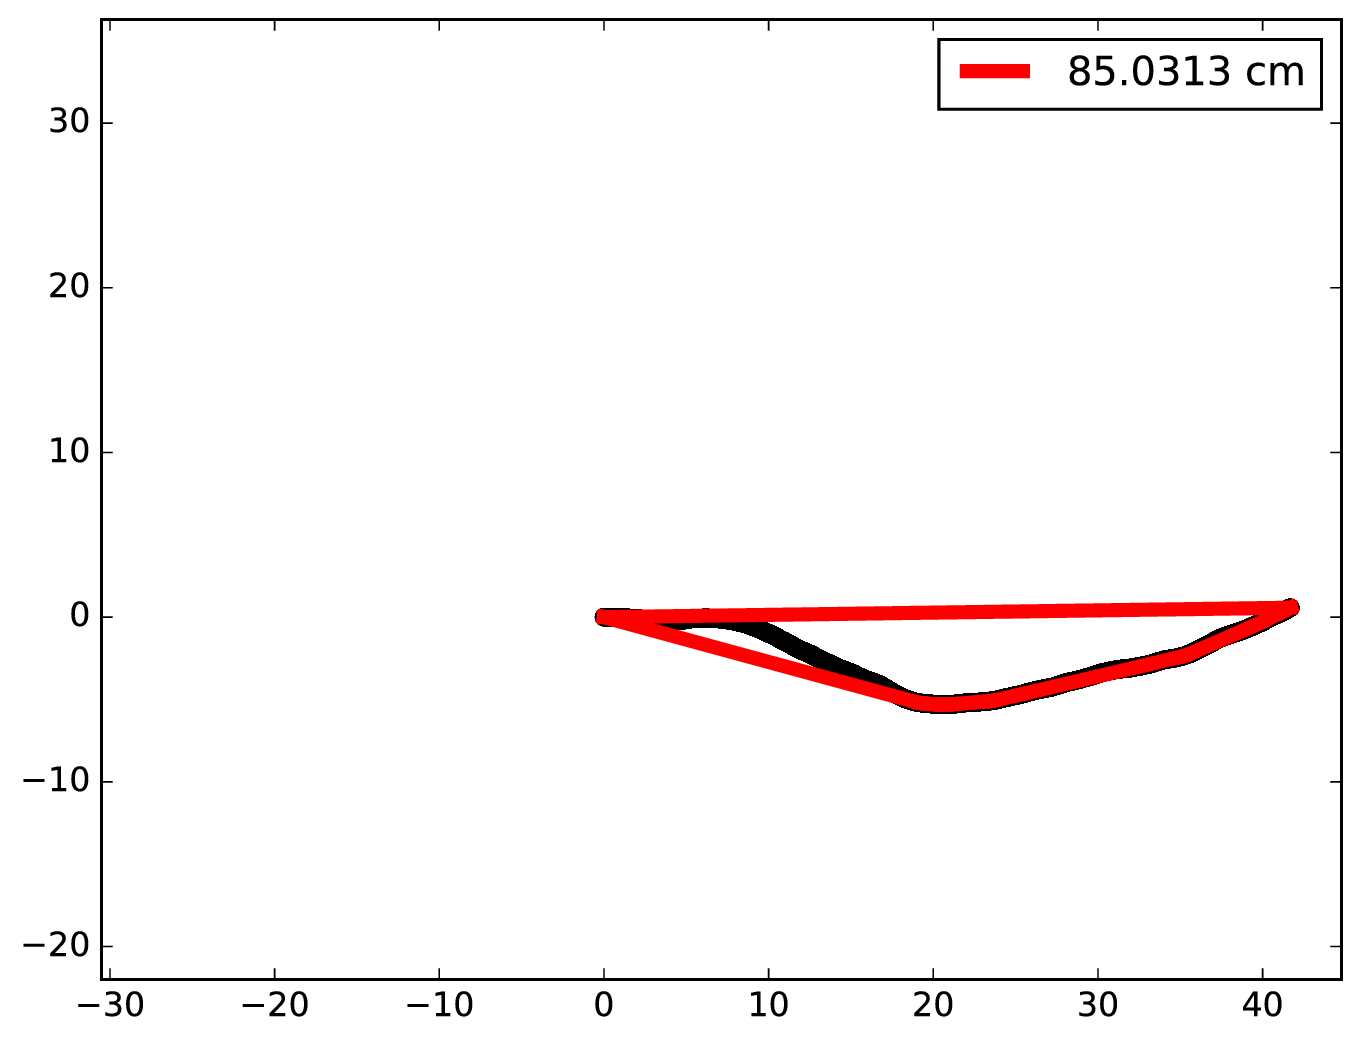
\includegraphics[width=\textwidth]{figures/ch3/areaTraj_2_19_5_8}
			\caption{$A = 5$, $F=8$, $AF=40$. $P\approx~85$~cm.}
			\label{fig:areaTraj_2_19_5_8}
		\end{subfigure}
		~
		\begin{subfigure}[t]{\subImgWmo}
			\centering
			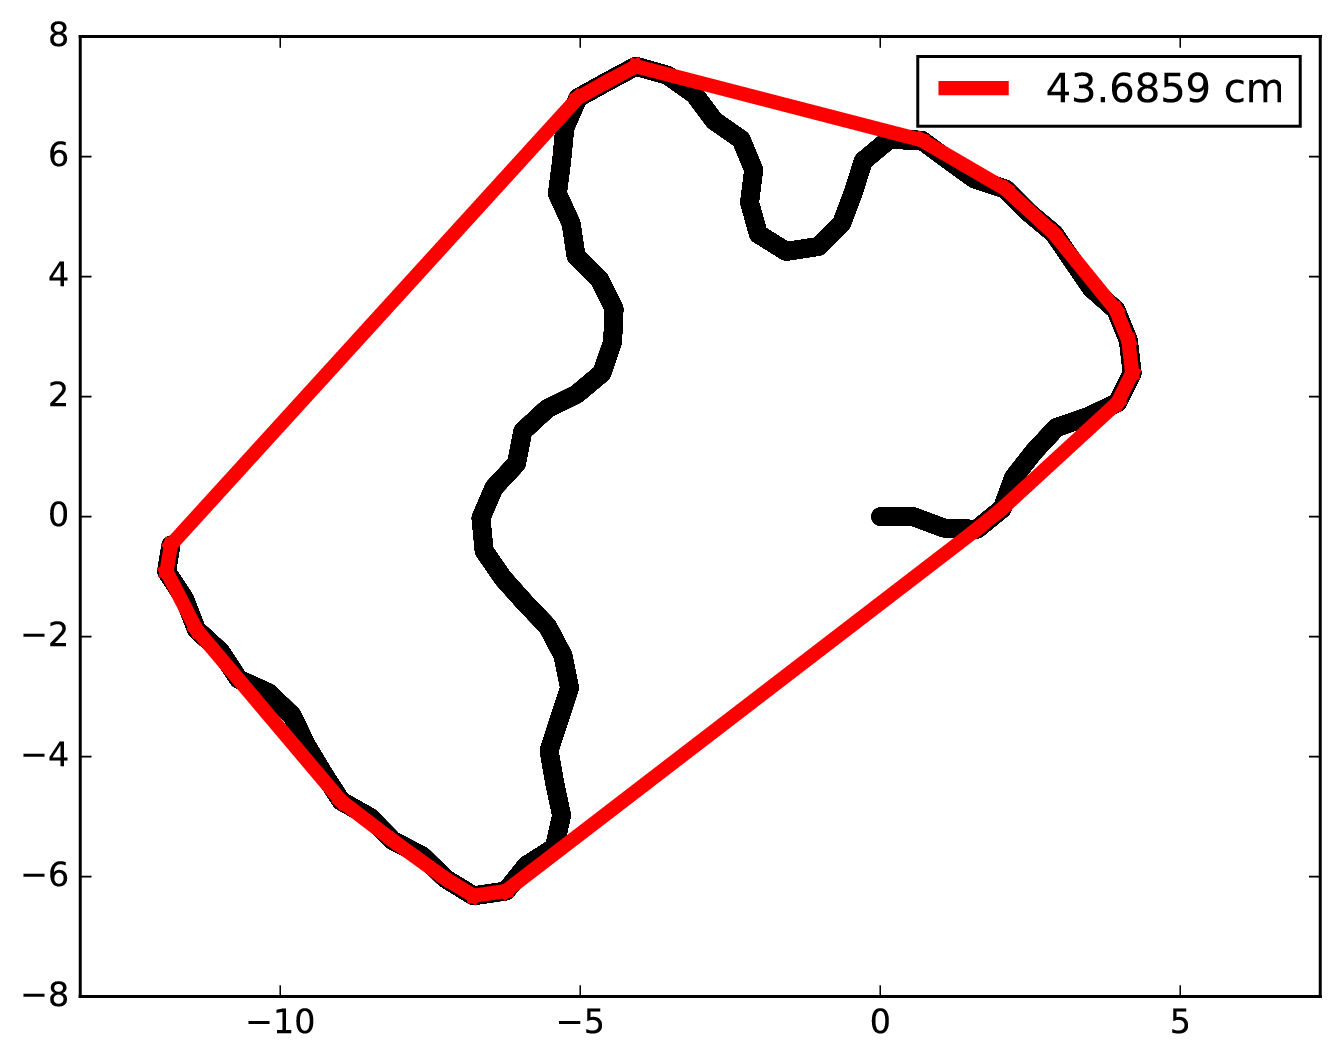
\includegraphics[width=\textwidth]{figures/ch3/areaTraj_2_19_45_4}
			\caption{$A = 45$, $F=4$, $AF=180$. $P\approx~53$~cm.}
			\label{fig:areaTraj_2_19_45_4}
		\end{subfigure}
		~
		\begin{subfigure}[t]{\subImgWmo}
			\centering
			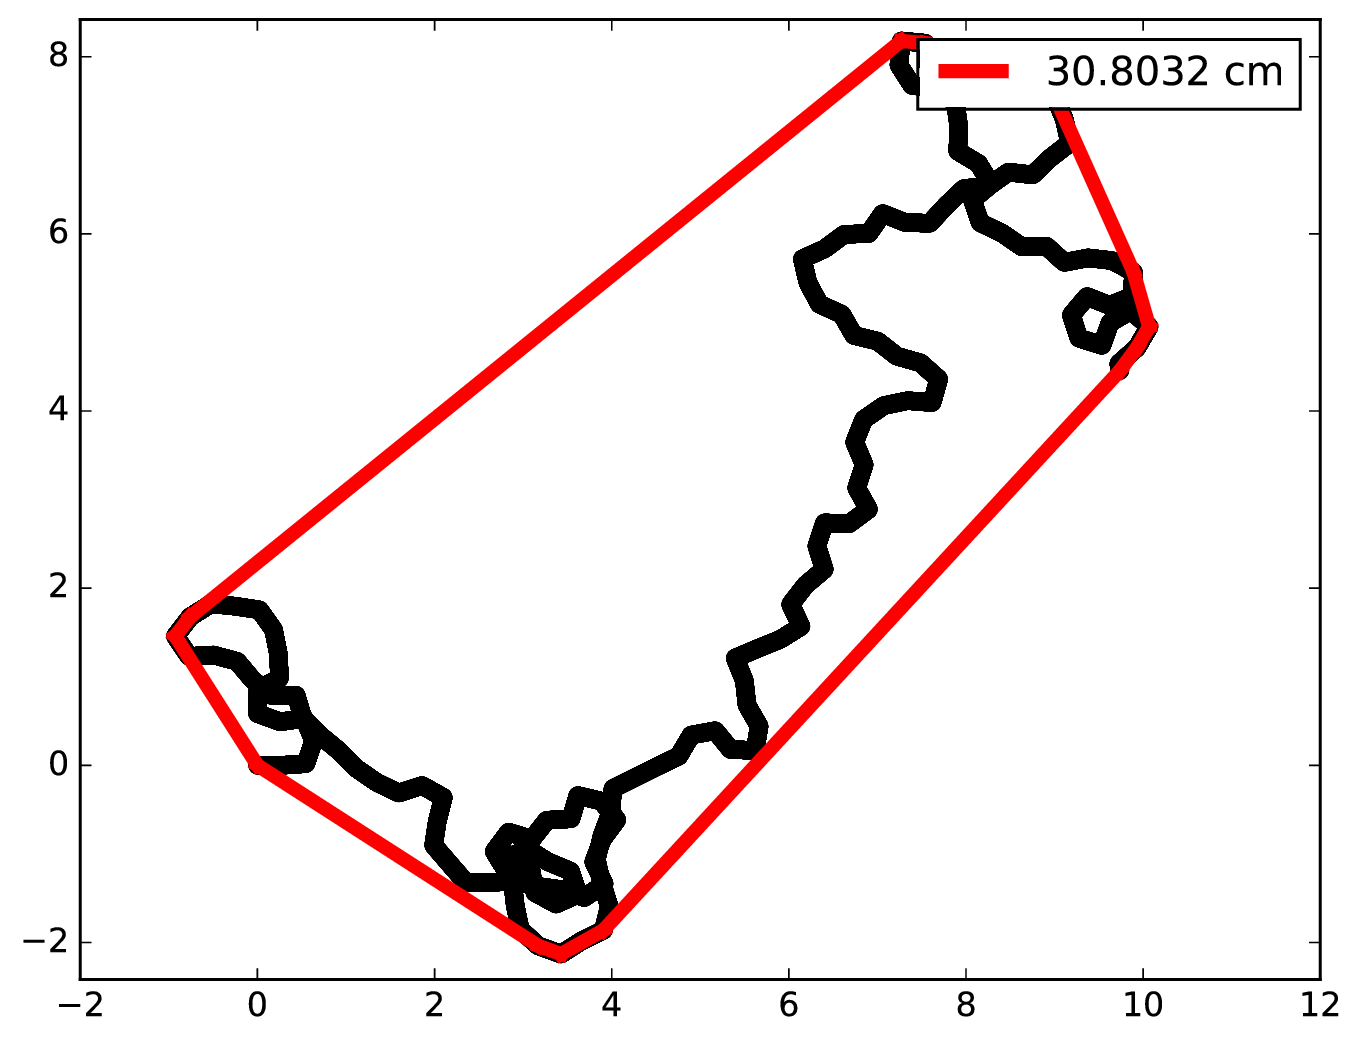
\includegraphics[width=\textwidth]{figures/ch3/areaTraj_2_19_90_8}
			\caption{$A = 90$, $F=8$, $AF=720$. $P\approx~16$~cm.}
			\label{fig:areaTraj_2_19_90_8}
		\end{subfigure}
		~
		\begin{subfigure}[t]{\subImgWmo}
			\centering
			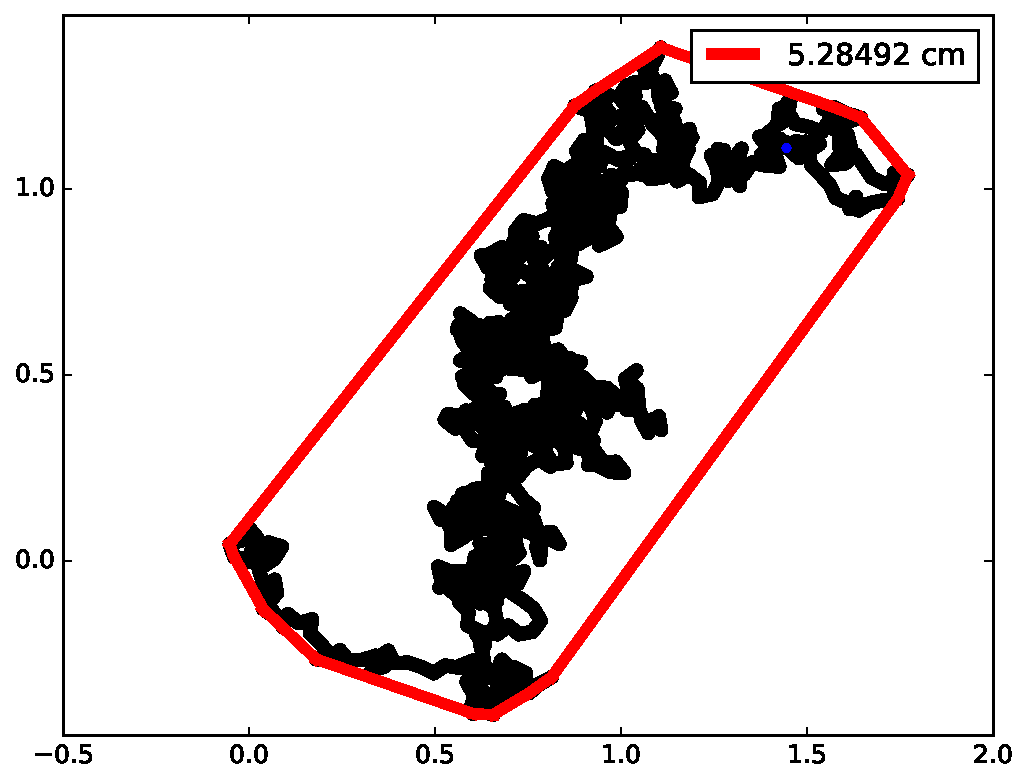
\includegraphics[width=\textwidth]{figures/ch3/areaTraj_2_19_180_60}
			\caption{$A = 180$, $F=60$, $AF=10800$. $P\approx~4$~cm.}
			\label{fig:areaTraj_2_19_180_60}
		\end{subfigure}
		~
		\begin{subfigure}[t]{\subImgWmo}
			\centering
			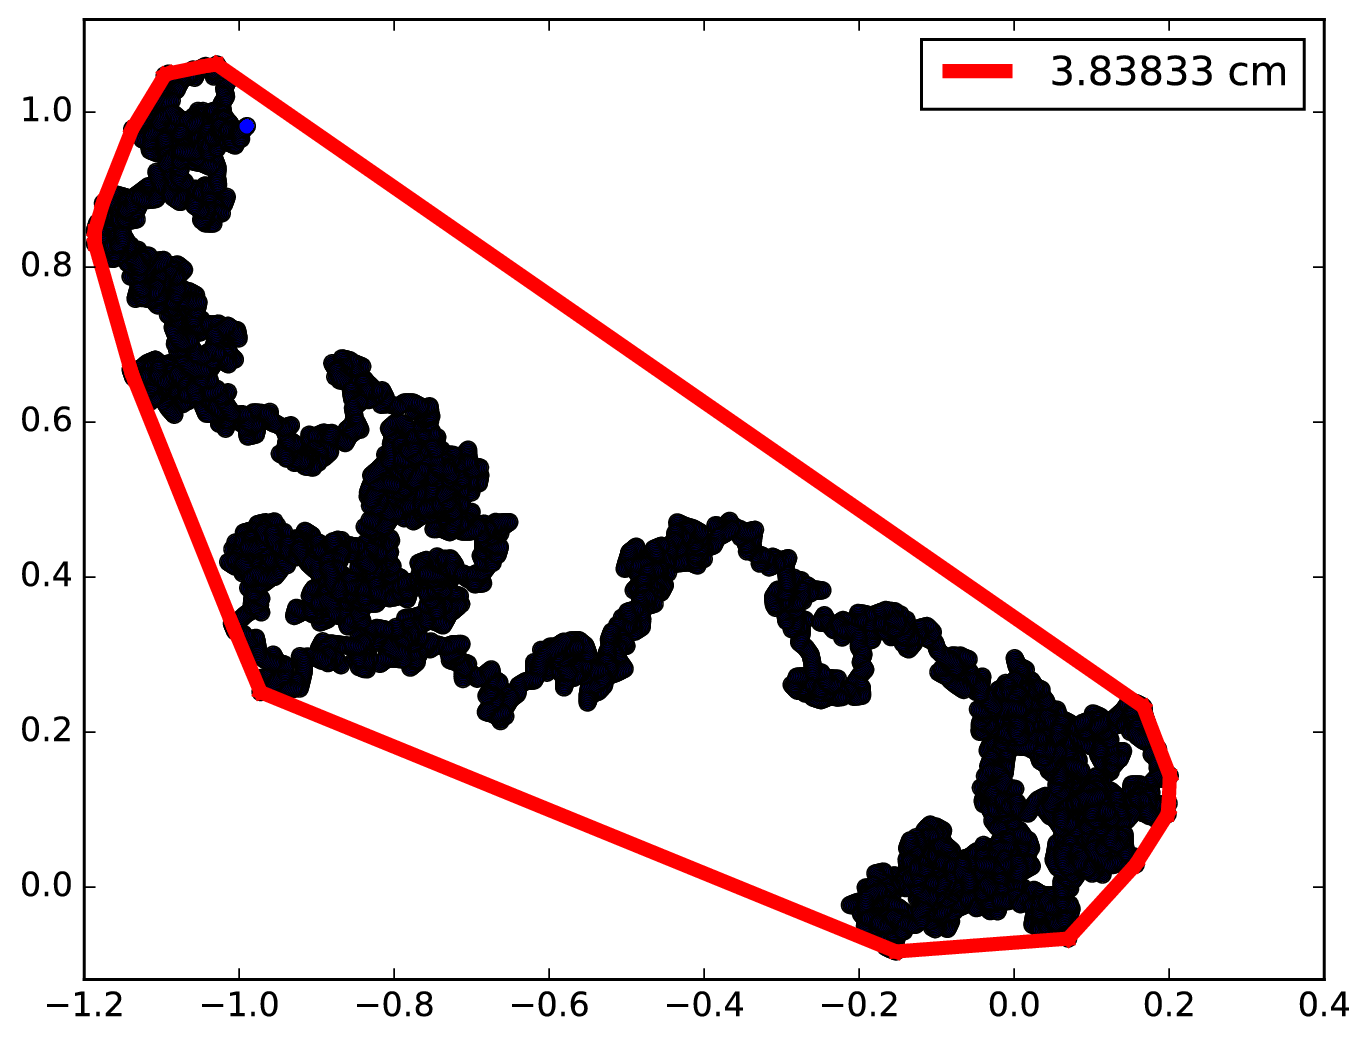
\includegraphics[width=\textwidth]{figures/ch3/areaTraj_2_19_180_240}
			\caption{$A = 180$, $F=240$, $AF=43200$. $P\approx~3$~cm.}
			\label{fig:areaTraj_2_19_180_240}
		\end{subfigure}
		\caption[Enveloppes convexes]{Enveloppes convexes de six trajectoires de pseudo-entropies croissantes. À mesure que la pseudo-entropie croît, elles sont de plus en plus \og repliées \fg{} et le périmètre $P$ de l'enveloppe convexe décroît.}
		\label{fig:trajAreas}
	\end{figure}
	
	L'on peut déduire de cette observation que si un utilisateur souhaite sélectionner une cible mobile de faible pseudo-entropie, il doit pouvoir atteindre, avec son curseur, tous les points d'une zone de taille importante, comme sur la figure~\ref{fig:areaTraj_2_19_1_16} ; à l'inverse, si la pseudo-entropie est élevée, la zone sera plus petite, comme sur la figure~\ref{fig:areaTraj_2_19_180_240}).
	
	Il serait tentant d'en déduire que la pseudo-entropie rend la sélection plus facile, mais n'oublions pas qu'elle implique un mouvement moins régulier, et donc plus imprévisible. Nous reviendrons en détail sur ce point plus loin. Observons simplement pour le moment que les trajectoires des figures~\ref{fig:areaTraj_2_19_1_16}, \ref{fig:areaTraj_2_19_5_8} et \ref{fig:areaTraj_2_19_45_4} (de pseudo-entropie maximale 180) sont nettement plus régulières --- donc prévisibles --- que la trajectoire de la figure~\ref{fig:areaTraj_2_19_90_8}, de pseudo-entropie 720. Il serait donc très imprudent de supposer que cette dernière correspond à une cible plus facile à sélectionner.
	
	Remarquons cependant que quand la pseudo-entropie est très faible, la régularité de la trajectoire suggère une sélection relativement aisée ; quand elle est très élevée, la très petite zone couverte par la trajectoire laisse également supposer une sélection assez facile, du fait d'une distance (telle que définie par Fitts~\cite{fitts1954information}) très courte, à partir du moment où le curseur atteint l'enveloppe convexe de la cible.
	
	\section{Validation de la taxinomie}
	Pour valider notre taxinomie des cibles mobiles et de leurs environnements, nous nous sommes appuyés sur des mesures quantitatives et objectives des critères les plus importants que nous avons retenus. Nous avons pour cela adopté deux approches complémentaires :
	
	\begin{itemize}
		\item Premièrement, nous avons développé une suite d'outils permettant de traiter des résultats bruts de simulations de dynamique moléculaire (appelés \emph{trajectoires}) afin de mesurer les angles de rotation des vecteurs direction des atomes, et d'analyser ces mesures ;
		\item Deuxièmement, nous avons développé une suite d'outils permettant d'annoter des vidéos contenant des cibles sur lesquelles l'utilisateur peut cliquer afin de marquer leurs positions dans le temps, et d'analyser les résultats.
	\end{itemize}

	Dans le premier cas, de très grandes quantités de données peuvent être traitées, en mesurant les angles en 3D, mais uniquement pour des simulations moléculaires. Dans le second, les vidéos peuvent représenter n'importe quel type de cible, mais nécessitent --- pour le moment --- un traitement manuel. L'ajout d'une méthode de reconnaissance d'objet permettrait de se passer de l'intervention d'un humain, mais devrait être très fiable pour être utilisable.
	
	\subsection{Analyses de \emph{trajectoires} de dynamique moléculaire}
	Une simulation de dynamique moléculaire cherche à déterminer le comportement d'un système sur une durée \emph{réelle} donnée, généralement de l'ordre de la nanoseconde. L'état du système (notamment les positions des atomes) est déterminé pour chaque pas de temps. En pratique, les résultats de la simulation peuvent ensuite être affichés avec un nombre de pas de temps par seconde arbitraire, ce qui implique que les vitesses des cibles dépendent du choix fait pour la visualisation.
	
	De même, les atomes sont susceptibles de changer de direction à chaque pas de temps, et c'est généralement le cas. La fréquence des changements de direction dépend donc également du nombre de pas par seconde lors de l'affichage des résultats.
	
	Les valeurs des angles de rotation des vecteurs direction, elles, sont indépendantes de ce choix, puisqu'il s'agit simplement, pour chaque atome, de l'écart entre son vecteur direction d'un pas à l'autre. C'est donc sur cette valeur que nous nous sommes concentrés, en gardant à l'esprit que la vitesse des cibles et la fréquence des changements de direction sont variables et dépendent du mode d'affichage choisi.
	
	Nous avons ainsi analysé un échantillon hétérogène de systèmes moléculaires. Cet échantillon est issu de nos échanges avec des spécialistes de la biologie structurale, et constitué par leurs soins : il est constitué de systèmes faisant l'objet de simulations \og réelles \fg{}, c'est-à-dire visant à répondre à des questions de recherche en biologie.
	
	Pour chaque simulation, nous mesurons tous les angles de rotation, pour chaque pas de temps. Pour chaque système, nous avons ensuite dressé un histogramme de toutes ces valeurs, afin d'avoir une représentation complète de toute la gamme d'angles possibles, et des proportions dans lesquelles ils apparaissent. Ces histogrammes sont présentés sur la figure~\ref{fig:dynMolAngles}.
	
	\newcommand{\subImgWaStats}{0.23\textwidth}
	\begin{figure}[htb]
		\begin{subfigure}[t]{\subImgWaStats}
			\centering
			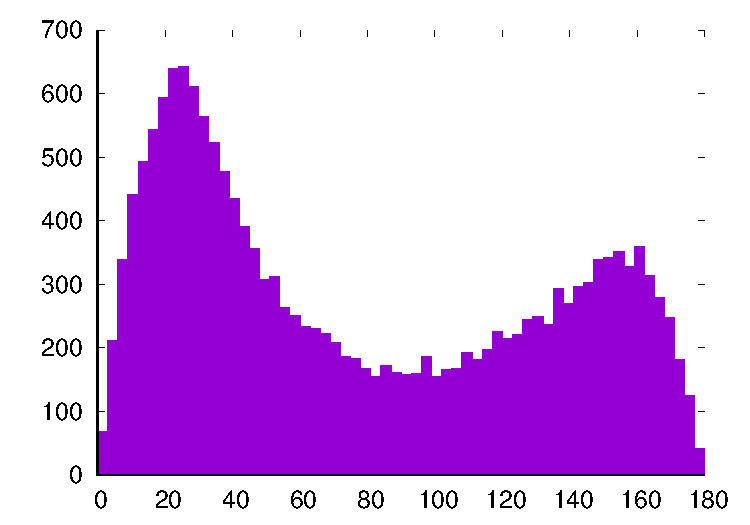
\includegraphics[width=\textwidth]{figures/ch3/02_DA_all_angles}
			\caption{}
			\label{fig:02_DA_all_angles}
		\end{subfigure}
		~
		\begin{subfigure}[t]{\subImgWaStats}
			\centering
			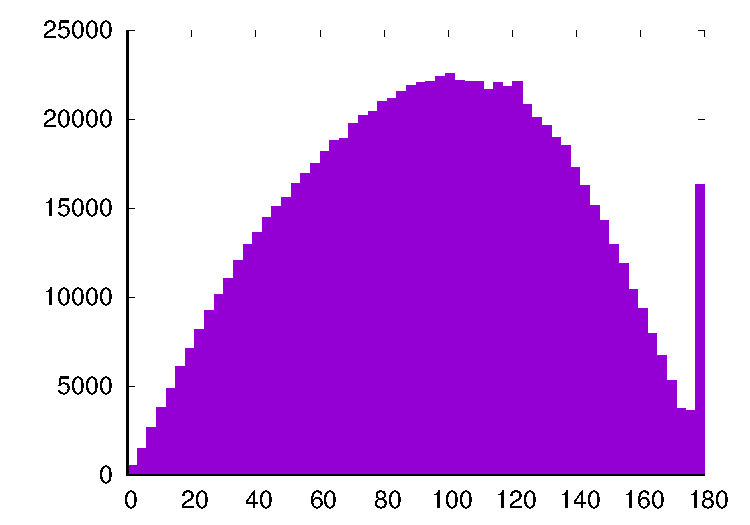
\includegraphics[width=\textwidth]{figures/ch3/148L_all_angles}
			\caption{}
			\label{fig:148L_all_angles}
		\end{subfigure}
		~
		\begin{subfigure}[t]{\subImgWaStats}
			\centering
			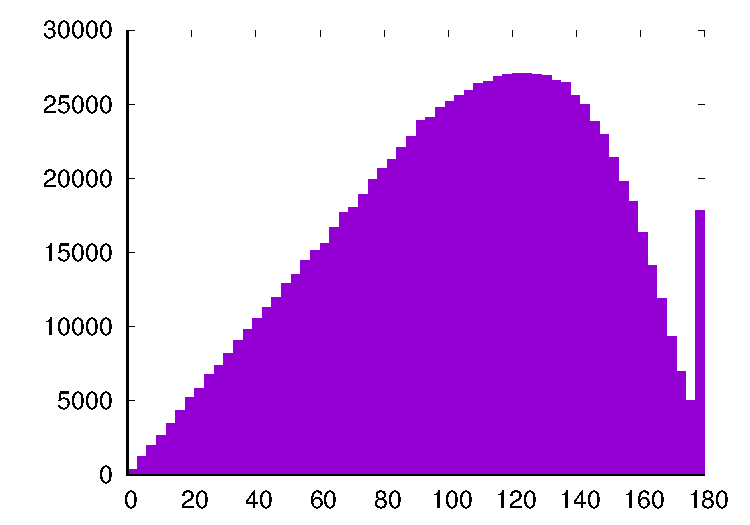
\includegraphics[width=\textwidth]{figures/ch3/snare_tmd_gg_all_angles}
			\caption{}
			\label{fig:snare_tmd_gg_all_angles}
		\end{subfigure}
		~
		\begin{subfigure}[t]{\subImgWaStats}
			\centering
			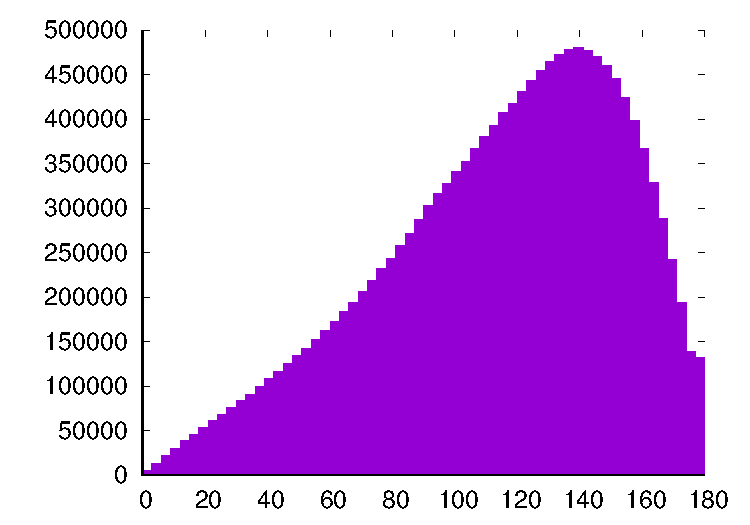
\includegraphics[width=\textwidth]{figures/ch3/gk_extension_all_angles}
			\caption{}
			\label{fig:gk_extension_all_angles}
		\end{subfigure}
		\caption[Angles de rotation, dynamique moléculaire]{Angles (en abscisse et en degrés) de rotation des vecteurs direction des atomes de simulations de dynamique moléculaire. Les nombres absolus d'occurrences sont en ordonnée, pour chacun des quatre systèmes analysés (a, b, c, et d.)}
		\label{fig:dynMolAngles}
	\end{figure}

	Sur cette figure, l'on constate que les angles mesurés ont généralement une distribution asymétrique, avec un cas particulier sur la figure~\ref{fig:02_DA_all_angles}, dont l'histogramme admet deux pics. Les lois mathématiques précises régissant ces distributions importent moins que leurs conséquences pratiques, qui découlent d'une part de l'intervalle des valeurs possibles ([0,180] sur tous les systèmes que nous avons étudiés), et d'autre part de leurs fréquences d'occurrence respectives.
	
	Premièrement, tous les angles possibles peuvent apparaître, et ce jusqu'à 180\textdegree{}. Non seulement ces très grands angles (assimilables à des demi-tours) ne sont pas rares, mais sur les systèmes des figures~\ref{fig:148L_all_angles} et~\ref{fig:snare_tmd_gg_all_angles}, ils sont même très fréquents, avec des pics très marqués à cet endroit de leurs histogrammes respectifs.
	
	Deuxièmement, les angles les plus fréquents peuvent être autour de 100\textdegree{} (figure~\ref{fig:148L_all_angles}), 130\textdegree{} (figure~\ref{fig:snare_tmd_gg_all_angles}), 140\textdegree{} (figure~\ref{fig:gk_extension_all_angles}) ou seulement 25\textdegree{} (figure~\ref{fig:02_DA_all_angles}).
	
	Par conséquent, l'interaction avec les (résultats de) simulations de dynamique moléculaire nécessite de pouvoir gérer des angles de rotation de n'importe quelle valeur, et même de s'adapter à des distributions pouvant être très différentes, avec des valeurs d'occurrence maximale pouvant prendre n'importe quelle valeur au sein d'un intervalle s'étendant au moins de 25\textdegree{} à 140\textdegree{}. Sur une autre simulation à très haute fréquence, nous avons même observé un histogramme entièrement borné par les valeurs 15\textdegree{} et 18\textdegree{} --- nous l'omettons ici, compte tenu du peu d'informations qu'il communique.
	
	Bien qu'il soit envisageable d'effectuer de telles analyses sur un très gros échantillon représentatif de \emph{trajectoires} de dynamique moléculaire, afin d'obtenir des statistiques détaillées, ce serait superflu par rapport à nos objectifs, qui consistent à caractériser les besoins de la tâche. Or, il apparaît que si l'on examine cette application au travers du prisme de notre modèle VFA :
	
	\begin{itemize}
		\item toutes les valeurs de V sont possibles, selon le mode d'affichage choisi,
		\item toutes les valeurs de F sont possibles, selon le mode d'affichage choisi,
		\item toutes les valeurs de A sont possibles, selon la nature du système et les paramètres de la simulation.
	\end{itemize}
	
	Par conséquent, les simulations de dynamique moléculaire peuvent potentiellement entrer dans toutes les catégories de mouvement markovien --- voire autocorrélé si la fréquence est suffisamment élevée. Mais surtout, les mouvements susceptibles de poser les plus grandes difficultés de sélection sont possibles dans cette application.
	
	\FloatBarrier \subsection{Analyses des mouvements d'objets divers}
	Au cours de cette phase, nous avons annoté des vidéos de types très divers pour caractériser quantitativement et objectivement le mouvement de cibles variées, telles qu'elles apparaissent à l'écran --- c'est-à-dire que nous avons mesurés les mouvements relatifs plutôt qu'absolus, attendu que ce sont ceux qui seraient effectivement perçu par un utilisateur. Nous avons ensuite analysé les résultats pour comptabiliser tous les angles de rotation de vecteur vitesse, toutes les fréquences de rotation, et toutes les vitesses. Nous avons donc pu construire des histogrammes pour chacune de ces grandeurs, mais aussi en calculer la moyenne, l'écart-type, et en noter la valeur maximale.
	
	Lorsqu'une vidéo représente plusieurs cibles potentielles, nos résultats correspondent à des mesures effectuées sur un échantillon de celles-ci. Les vidéos elles-mêmes furent choisies en recherchant la plus grande diversité possible, et en privilégiant les mouvements vifs et imprévisibles, car il s'agit des cas les plus intéressants, du fait de la difficulté inhérente à la sélection de tels objets. Nous incluons néanmoins plusieurs vidéos d'objets lents, ou de mouvements réguliers et prévisibles.
	
	
	Avant d'exposer et commenter nos résultats, il convient de noter que les fréquences de changements de direction mesurées ici sont significativement affectées par le nombre d'images par seconde dans les vidéos utilisées comme sources. Celles-ci ont généralement une fréquence de 24~Hz ou 30~Hz, qui peut être insuffisante pour correctement échantillonner les véritables fréquences de changement de direction des cibles observées, si elles dépassent 12~Hz ou 15~Hz, respectivement~\cite{shannon1949communication}. La prudence s'impose donc pour l'interprétation de nos résultats concernant cette caractéristique du mouvement ; cette réserve ne s'applique pas aux vitesses, et nettement moins aux angles.
	
	Par ailleurs, la nature intrinsèquement discrète des vidéos, constituées d'un nombre donné d'images par seconde, implique une discrétisation \emph{de facto} de mouvements qui, en soi, peuvent être ciné-continus. La lecture de ces résultats impose de garder à l'esprit qu'ils ne reflètent pas directement la nature réelle des mouvements mesurés. Mais puisque les tâches de sélection impliquent presque toujours un système interactif opérant une discrétisation semblable, nos mesures demeurent pertinentes d'un point de vue pratique et applicatif. De plus, le grand nombre (plus de 116~000) d'images annotées nous permet de prétendre à une certaine représentativité.
	
	Pour commencer, nous avons annoté un enregistrement vidéo d'une simulation de dynamique moléculaire, avec une petite molécule. Les résultats que nous avons obtenus sont présentés sous forme d'histogrammes de vitesses (figure~\ref{fig:atom_filteredSpeed}), de fréquences (figure~\ref{fig:atom_frequency}), et d'angles (figure~\ref{fig:atom_angle}) d'une part ; et sur la table~\ref{tab:atom_stats} d'autre part. Sur cette dernière et sur toutes les tables de cette section figurent la vitesse maximale enregistrée ($V_{max}$), la vitesse moyenne ($\overline{V}$), l'écart-type des vitesses, ($\sigma_{V}$), la fréquence maximale ($F_{max}$), la fréquence moyenne ($\overline{F}$), l'écart-type des fréquences ($\sigma_{F}$), l'angle maximal ($A_{max}$), l'angle moyen ($\overline{A}$), et enfin l'écart-type des angles ($\sigma_{A}$). Sur les histogrammes comme sur les tables, les vitesses sont en cm/s, les fréquences en Hz, et les angles en degrés. Les résultats sont cohérents avec nos mesures sur des données brutes de simulation, et illustrent bien à quel point les cibles de ce type peuvent être difficiles à saisir.
	
	\newcommand{\subImgWclicks}{0.32\textwidth}
	
	\begin{figure}[!htbp]
		\begin{subfigure}[t]{\subImgWclicks}
			\centering
			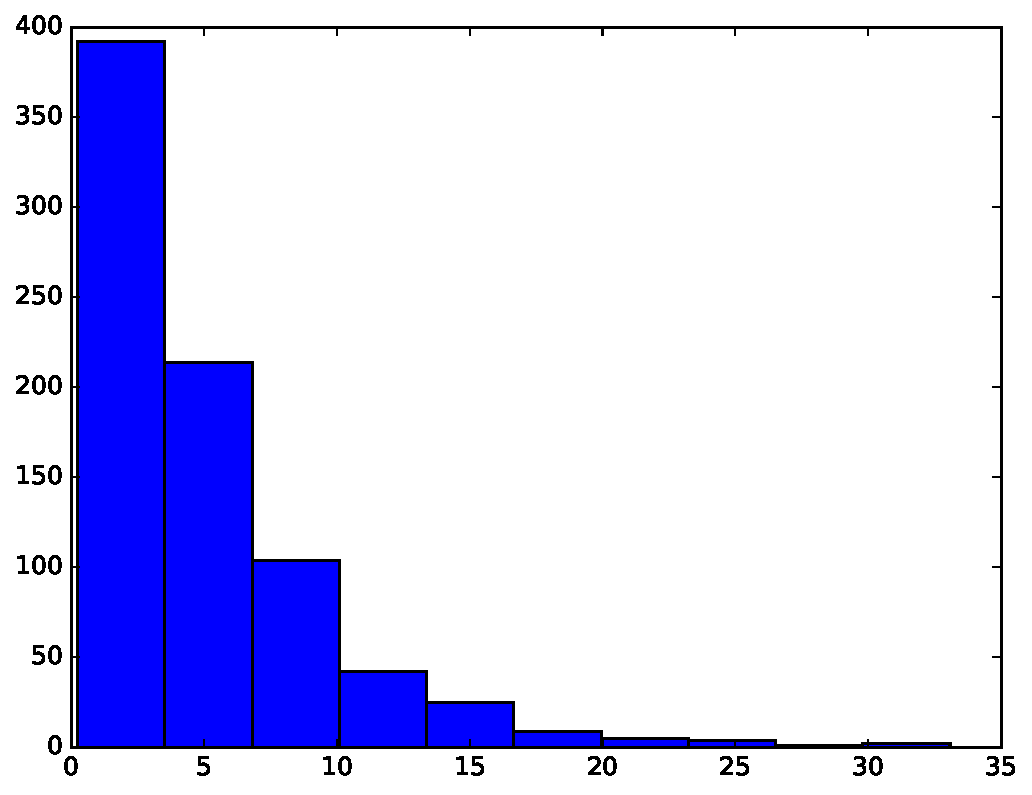
\includegraphics[width=\textwidth]{figures/ch3/atom_filteredSpeed}
			\caption{Vitesses.}
			\label{fig:atom_filteredSpeed}
		\end{subfigure}
		~
		\begin{subfigure}[t]{\subImgWclicks}
			\centering
			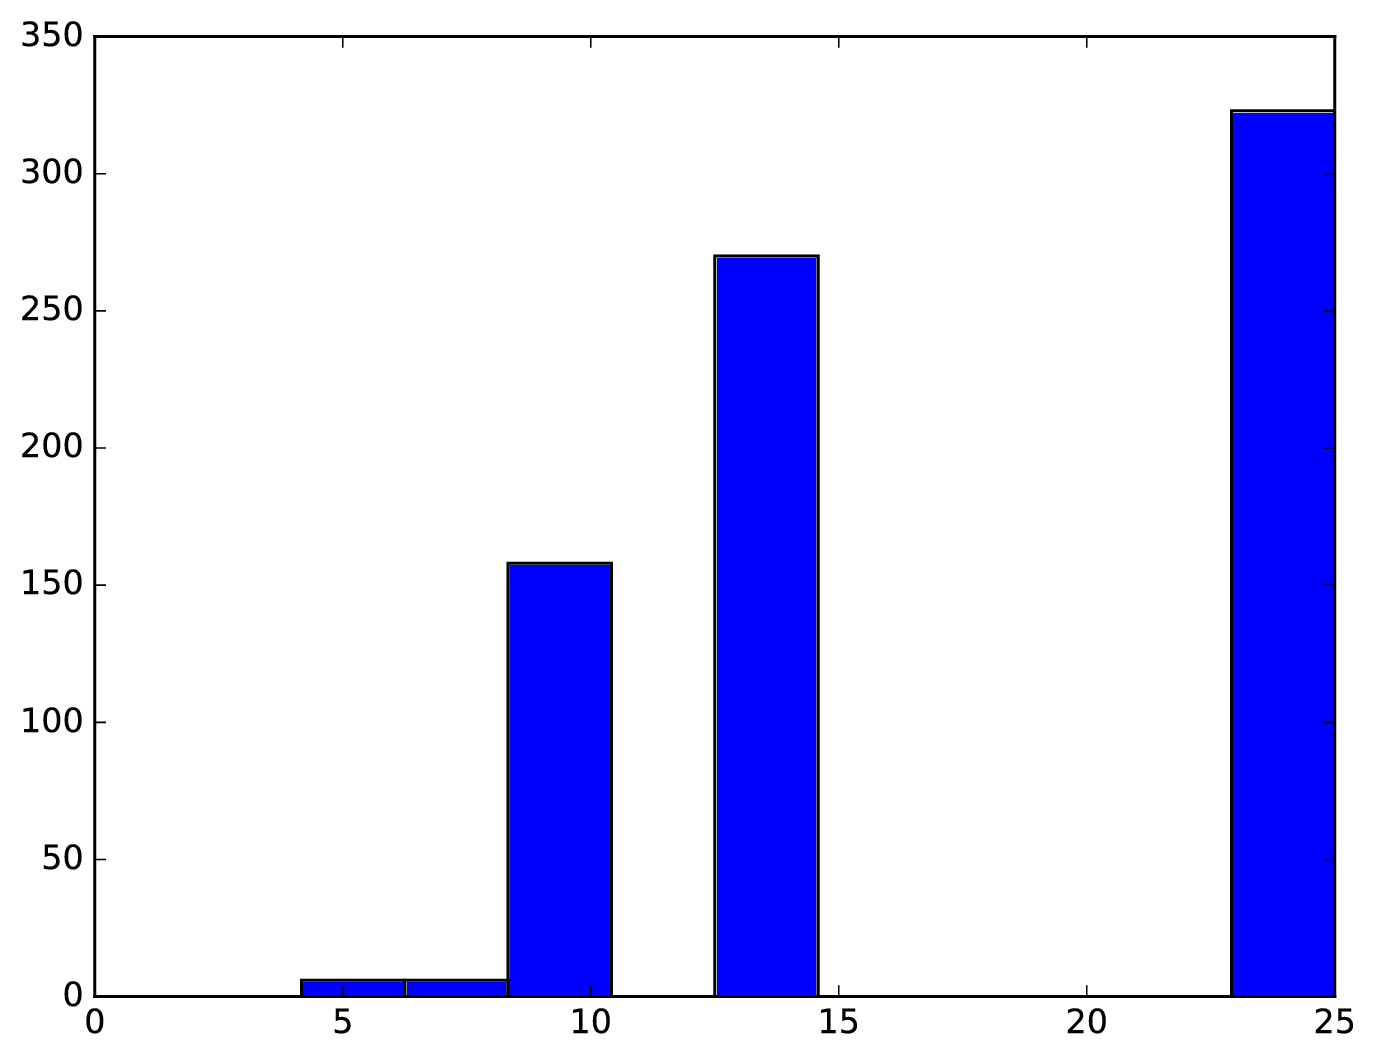
\includegraphics[width=\textwidth]{figures/ch3/atom_frequency}
			\caption{Fréquences.}
			\label{fig:atom_frequency}
		\end{subfigure}
		~
		\begin{subfigure}[t]{\subImgWclicks}
			\centering
			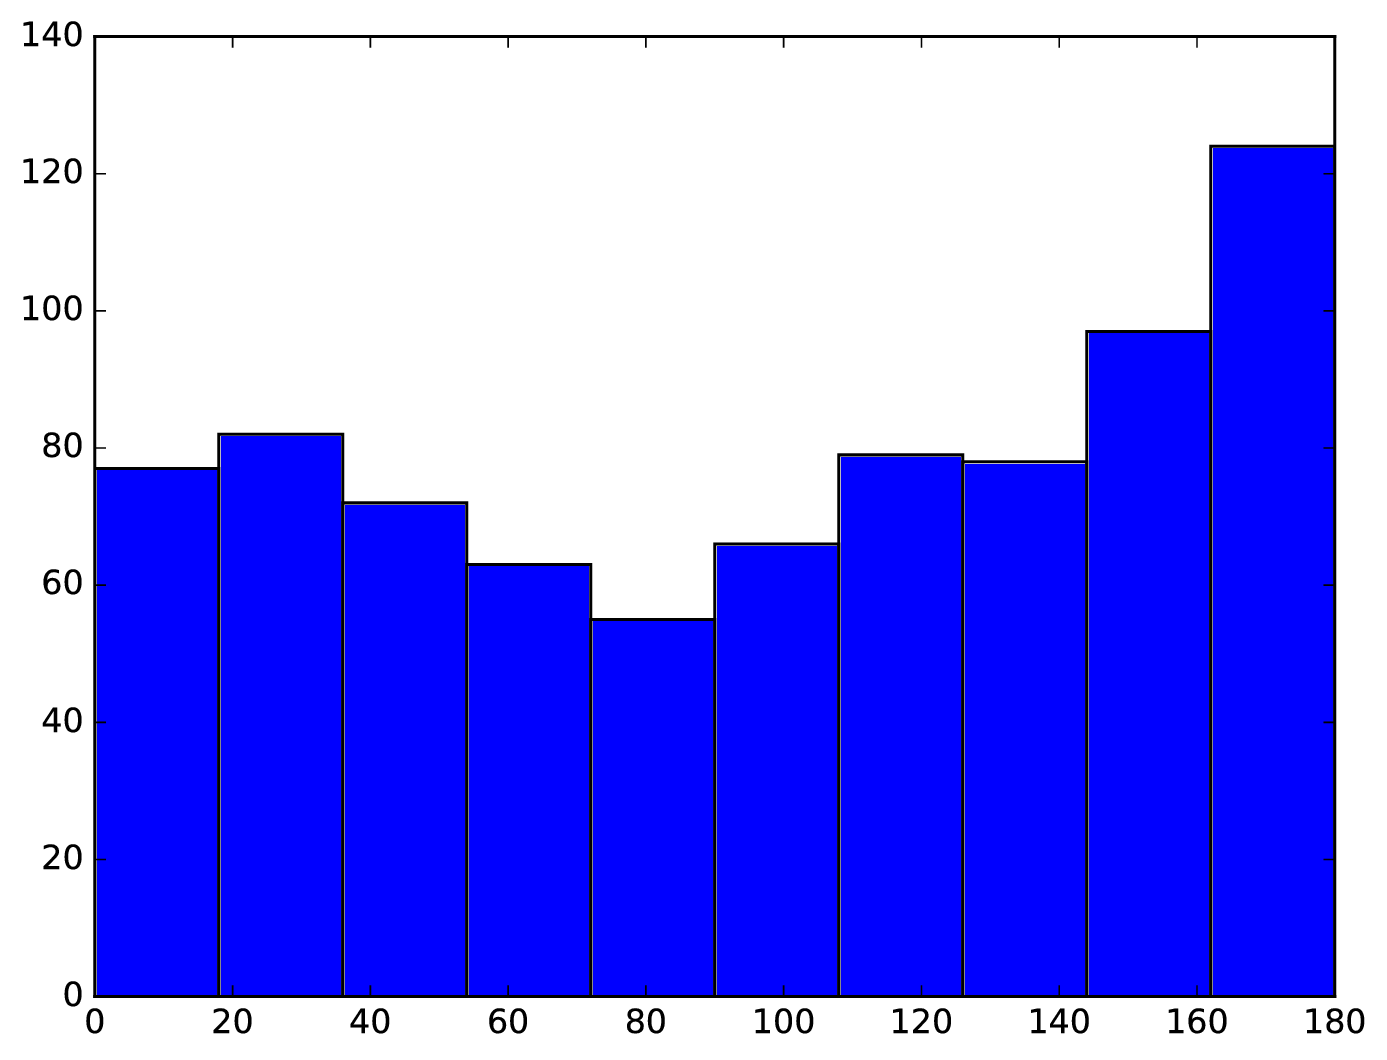
\includegraphics[width=\textwidth]{figures/ch3/atom_angle}
			\caption{Angles.}
			\label{fig:atom_angle}
		\end{subfigure}
		\caption[Histogrammes pour la dynamique moléculaire]{Histogrammes pour la dynamique moléculaire.}
		\label{fig:histAtoms}
	\end{figure}

\begin{table}
	\centering
	\begin{tabular}{c c c c c c c c c}
		$V_{max}$	& $\overline{V}$	& $\sigma_{V}$	& $F_{max}$	& $\overline{F}$	& $\sigma_{F}$	& $A_{max}$	& $\overline{A}$	& $\sigma_{A}$	\bigstrut[b] \\ \hline

		33,08		& 4,84				& 4,60			& 25,00		& 16,82				& 7,20			& 180,00	& 96,98				& 55,86			\bigstrut[t] \\
	\end{tabular}
	\caption[Statistiques pour la vidéo de dynamique moléculaire]{Statistiques pour la vidéo de dynamique moléculaire.}
	\label{tab:atom_stats}
\end{table}	

	Ensuite, nous avons annoté un enregistrement vidéo d'un avion de ligne, filmé depuis le sol avec une caméra suivant l'appareil, tenue à la main, ce qui implique de fréquentes saccades. Les histogrammes correspondants sont sur les figures~\ref{fig:chinaA_filteredSpeed}, \ref{fig:chinaA_frequency}, et \ref{fig:chinaA_angle} ; la table~\ref{tab:chinaA_stats} synthétise ces résultats.

	\begin{figure}[!htbp]
		\begin{subfigure}[t]{\subImgWclicks}
			\centering
			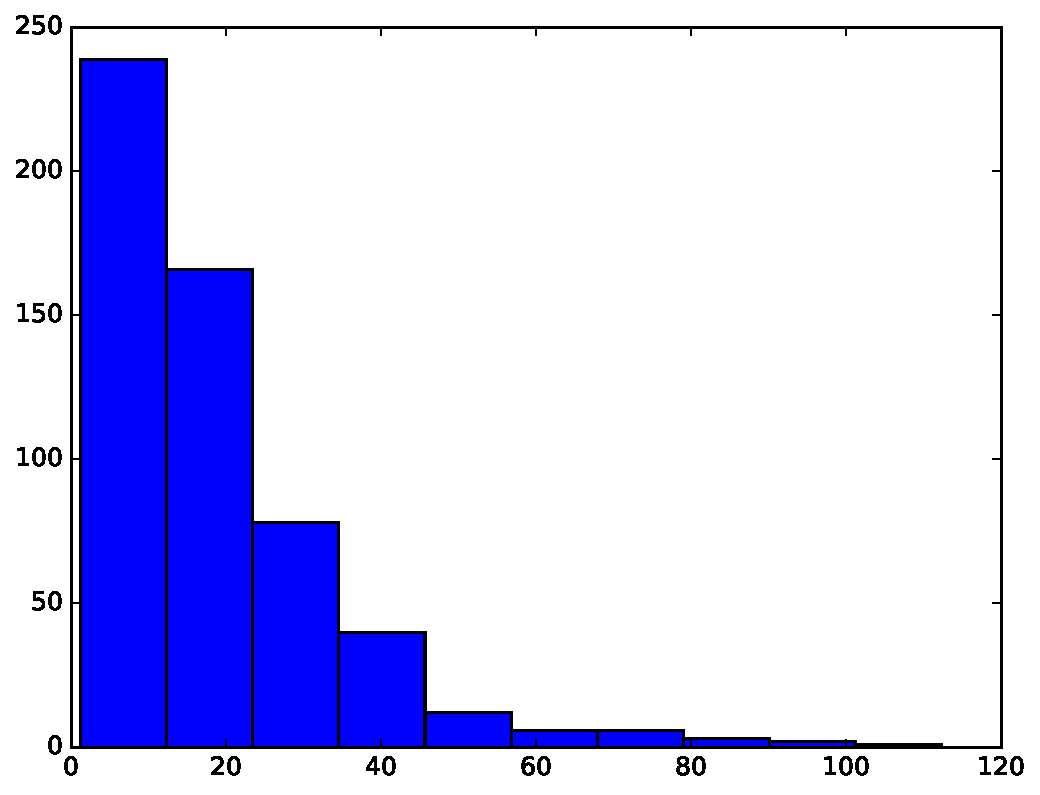
\includegraphics[width=\textwidth]{figures/ch3/chinaA_filteredSpeed}
			\caption{Vitesses.}
			\label{fig:chinaA_filteredSpeed}
		\end{subfigure}
		~
		\begin{subfigure}[t]{\subImgWclicks}
			\centering
			\includegraphics[width=\textwidth]{figures/ch3/chinaA_frequency}
			\caption{Fréquences.}
			\label{fig:chinaA_frequency}
		\end{subfigure}
		~
		\begin{subfigure}[t]{\subImgWclicks}
			\centering
			\includegraphics[width=\textwidth]{figures/ch3/chinaA_angle}
			\caption{Angles.}
			\label{fig:chinaA_angle}
		\end{subfigure}
		\caption[Histogrammes pour l'avion de ligne]{Histogrammes pour l'avion de ligne.}
		\label{fig:histChina}
	\end{figure}
	
\begin{table}
	\centering
	\begin{tabular}{c c c c c c c c c}
		$V_{max}$	& $\overline{V}$	& $\sigma_{V}$	& $F_{max}$	& $\overline{F}$	& $\sigma_{F}$	& $A_{max}$	& $\overline{A}$	& $\sigma_{A}$	\bigstrut[b] \\ \hline

		112,36		& 18,21				& 16,26			& 59,96		& 17,50				& 17,39			& 180,00	& 55,42				& 52,50			\bigstrut[t] \\
	\end{tabular}
	\caption[Statistiques pour la vidéo de l'avion de ligne]{Statistiques pour la vidéo de l'avion de ligne.}
	\label{tab:chinaA_stats}
\end{table}

	Les petites vitesses sont majoritaires, notamment car la caméra suit la cible, mais les vitesses élevées sont loin d'être rares, notamment du fait de saccades dans la vidéo. La plupart des angles sont faibles mais l'abondance de saccades mène à une distribution assez \og plate \fg{} une fois les petits angles écartés.

	Sur le même thème, nous avons annoté une vidéo de l'éphémère vol du \emph{Concorde} qui s'écrasa à Gonesse en juillet 2000\footnotemark{}. Les histogrammes sont sur les figures~\ref{fig:concordeA_filteredSpeed}, \ref{fig:concordeA_frequency}, et \ref{fig:concordeA_angle} ; la table~\ref{tab:concordeA_stats} synthétise ces résultats. Ici encore et pour les mêmes raisons, les vitesses faibles sont majoritaires mais de nombreuses valeurs élevées furent enregistrées. Les angles sont le plus souvent petits mais parfois beaucoup plus grands. De même, les valeurs proches de 180\textdegree{} s'expliquent par le fait que la caméra peut anticiper les mouvements de la cible, ce qui implique un demi-tour de celle-ci dans le référentiel de l'écran.
	
	\footnotetext{\url{https://www.bea.aero/docspa/2000/f-sc000725/pdf/f-sc000725.pdf}}

	Nous soulignions au cours du chapitre~\ref{chap1} l'intérêt des mouvements de foule --- manifestations, émeutes, etc. Aussi avons-nous annoté deux vidéos d'émeutes, dont les histogrammes sont représentés sur la figure~\ref{fig:histRiots}, et dont les résultats synthétiques sont sur les tables~\ref{tab:riot_stats} et \ref{tab:riot2a_stats}. Sur ces vidéos, les vitesses sont un peu plus faibles, les valeurs plus élevées étant généralement liées aux charges et autres courses rapides. Les fréquences sont plutôt basses et les angles distribués de façon approximativement uniforme, exception faite des petits angles, sur-représentés, comme c'est souvent le cas. Les deux vidéos produisent des résultats assez cohérents entre eux, ce qui est logique attendu qu'il s'agit d'événements du même type.



	Le contrôle du trafic aérien est une application doublement intéressante : d'une part du fait des caractéristiques de ses cibles, et d'autre part du fait de son caractère critique ; c'est pourquoi nous avons choisi d'en annoter plusieurs vidéos. Pour deux d'entre elles, les histogrammes sont présentés sur la figure~\ref{fig:histAirControl12}, tandis que les statistiques synthétiques sont disponibles dans les tables~\ref{tab:mhA_stats} et \ref{tab:germanwingsA_stats}. Les vitesses sont généralement très basses et stables, ce qui est logique puisque les avions sont observés sur une très grande échelle, et en vol de croisière. Toutefois, elles sont parfois très élevées, en particulier quand le point de vue est déplacé ou en cas de zoom ; c'est là qu'il faut chercher l'explication du second pic, à 5~cm/s, sur la figure~\ref{fig:germanwingsA_filteredSpeed}. Pour les mêmes raisons, les fréquences sont assez faibles, mais les grands angles ne sont pas rares, même si les petits sont largement majoritaires. Là encore, la raison est essentiellement à chercher du côté des ajustements du point de vue.	

	Nous avons annoté deux vidéos de plus pour le trafic aérien, dont les histogrammes sont sur la figure~\ref{fig:histAirControl34} et les statistiques synthétiques sur les tables~\ref{tab:hkg_stats} et \ref{tab:flightradar2a_stats}. Les résultats sont cohérents avec ceux des vidéos précédentes, ce qui nous fournit une caractérisation assez complète et précise des tâches de sélection de cibles mobiles pour le contrôle du trafic aérien. Certes, ces vidéos sont issues d'outils publics tels que \emph{FlightRadar24} plutôt que d'applications professionnelles, mais le fonctionnement des premiers est proche de celui des secondes.

	Il ressort de ces observations que les cibles ne sont pas intrinsèquement très difficiles à sélectionner avec ces outils, mais par leur nombre, la densité et l'occultation qui en résultent, elles peuvent présenter des difficultés significatives. Ajoutons, après avoir consulté la table~\ref{tab:flightradar2a_stats}, que les vitesses maximales peuvent être élevées, notamment lors de modifications du point de vue ou zooms. Outre l'effet perturbant que de tels pics de vitesse peuvent avoir, notamment par la discontinuité qu'ils introduisent, ils rendent une éventuelle tâche de sélection bien plus difficile, ne serait-ce que ponctuellement.
	
	Les avions ne sont pas les seuls objets volants pouvant faire l'objet d'une tâche de sélection, et c'est pourquoi nous avons aussi annoté une vidéo de la navette spatiale américaine (\emph{Space shuttle} ou \emph{Space Transportation System}, STS). Les histogrammes correspondants sont sur la figure~\ref{fig:histSpace}, tandis que les statistiques synthétiques sont dans la table~\ref{tab:spaceA_stats}. La distribution des vitesses est caractéristique des vidéos de ce type : dominée par les petites valeurs, avec quelques grandes valeurs liées aux saccades de la vidéo. Les fréquences présentent également un profil habituel, mais la distribution des angles est plus intéressante par son caractère relativement équilibré, avec beaucoup de grands angles, malgré une majorité de petits --- d'où des phases de mouvement assez diversifiées.
	
	Dans le domaine aérien, mais cette fois-ci vivant, nous avons annoté une vidéo d'un court vol d'oiseau (un pigeon), dont les histogrammes sont sur la figure~\ref{fig:histOiseau}, et les statistiques synthétiques dans la table~\ref{tab:oiseau_stats}. Les oiseaux en particulier, et les animaux en général pourraient faire l'objet de tâches de sélection de cible mobile dans des applications de réalité augmentée permettant de choisir un individu pour que le système reconnaisse automatiquement son espèce, sa race, et affiche des informations complémentaires tirées d'une base de données, voire d'une encyclopédie en ligne.

	Suivi par la caméra, le volatile génère surtout d'assez petites vitesses, d'autant que la vidéo est au ralenti. Ses distributions de fréquences et d'angles indiquent un mouvement de faible pseudo-entropie, donc relativement prévisible.
	
	Pour compléter ces données, nous avons annoté une deuxième courte vidéo du même type : le décollage d'un petit oiseau au ralenti. Les histogrammes sont sur la figure~\ref{fig:histBird}, et les statistiques synthétiques dans la table~\ref{tab:bird_stats}. Les résultats sont tout à fait cohérents avec ceux du pigeon, ce qui est logique attendu que les deux vidéos montrent un décollage, sont courtes, et filmées au ralenti.

	Dans la même veine que les oiseaux, et pour les mêmes raisons, nous avons annoté une vidéo d'un poisson dans un aquarium, face à une caméra fixe. Les histogrammes sont présentés sur la figure~\ref{fig:histPoisson}, et les statistiques synthétiques peuvent être consultées dans la table~\ref{tab:poisson_stats}.
	
	\begin{figure}[!htbp]
		\begin{subfigure}[t]{\subImgWclicks}
			\centering
			\includegraphics[width=\textwidth]{figures/ch3/poisson_filteredSpeed}
			\caption{Vitesses.}
			\label{fig:poisson_filteredSpeed}
		\end{subfigure}
		~
		\begin{subfigure}[t]{\subImgWclicks}
			\centering
			\includegraphics[width=\textwidth]{figures/ch3/poisson_frequency}
			\caption{Fréquences.}
			\label{fig:poisson_frequency}
		\end{subfigure}
		~
		\begin{subfigure}[t]{\subImgWclicks}
			\centering
			\includegraphics[width=\textwidth]{figures/ch3/poisson_angle}
			\caption{Angles.}
			\label{fig:poisson_angle}
		\end{subfigure}
		\caption[Histogrammes pour le poisson]{Histogrammes pour le poisson.}
		\label{fig:histPoisson}
	\end{figure}
	
\begin{table}
	\centering
	\begin{tabular}{c c c c c c c c c}
		$V_{max}$	& $\overline{V}$	& $\sigma_{V}$	& $F_{max}$	& $\overline{F}$	& $\sigma_{F}$	& $A_{max}$	& $\overline{A}$	& $\sigma_{A}$	\bigstrut[b] \\ \hline

		101,05		& 14,66				& 11,37			& 30,00		& 10,40				& 9,38			& 179,41	& 59,79				& 51,17			\bigstrut[t] \\
	\end{tabular}
	\caption[Statistiques pour la vidéo du poisson]{Statistiques pour la vidéo du poisson.}
	\label{tab:poisson_stats}
\end{table}

	Sans surprise, les vitesses sont généralement faibles, mais on constate une part non négligeable de vitesses relativement élevées (au-delà de 20~cm/s) intéressantes en ce qu'elles ne peuvent être imputées aux mouvements de la caméra, attendu que celle-ci était statique. Malgré une majorité de petits angles, on en trouve beaucoup de grands, encore une fois uniquement liés aux mouvements du poisson.	
	
	Le jeu vidéo fait partie des principales applications impliquant de difficiles tâches de sélection de cibles mobiles ; aussi en avons-nous annoté quelques vidéos, en commençant par une scène d'\emph{Empires of the Undergrowth}, un jeu de tactique en temps réel. Les histogrammes correspondants sont sur la figure~\ref{fig:histSpider}, et les statistiques de synthèse dans la table~\ref{tab:spider_stats}.

	\begin{figure}[!htbp]
		\begin{subfigure}[t]{\subImgWclicks}
			\centering
			\includegraphics[width=\textwidth]{figures/ch3/spider_filteredSpeed}
			\caption{Vitesses.}
			\label{fig:spider_filteredSpeed}
		\end{subfigure}
		~
		\begin{subfigure}[t]{\subImgWclicks}
			\centering
			\includegraphics[width=\textwidth]{figures/ch3/spider_frequency}
			\caption{Fréquences.}
			\label{fig:spider_frequency}
		\end{subfigure}
		~
		\begin{subfigure}[t]{\subImgWclicks}
			\centering
			\includegraphics[width=\textwidth]{figures/ch3/spider_angle}
			\caption{Angles.}
			\label{fig:spider_angle}
		\end{subfigure}
		\caption[Histogrammes pour le jeu \emph{Empires of the Undergrowth}]{Histogrammes pour le jeu \emph{Empires of the Undergrowth}.}
		\label{fig:histSpider}
	\end{figure}

\begin{table}
	\centering
	\begin{tabular}{c c c c c c c c c}
		$V_{max}$	& $\overline{V}$	& $\sigma_{V}$	& $F_{max}$	& $\overline{F}$	& $\sigma_{F}$	& $A_{max}$	& $\overline{A}$	& $\sigma_{A}$	\bigstrut[b] \\ \hline

		232,18		& 10,52				& 17,29			& 29,97		& 17,94				& 11,29			& 180,00	& 68,62				& 63,39			\bigstrut[t] \\
	\end{tabular}
	\caption[Statistiques pour la vidéo du jeu \emph{Empires of the Undergrowth}]{Statistiques pour la vidéo du jeu \emph{Empires of the Undergrowth}.}
	\label{tab:spider_stats}
\end{table}

	Si les vitesses ne sont pas énormes, elles dépassent occasionnellement la dizaine de cm/s (ce qui peut être dû à un déplacement du point de vue du joueur) avec de rares valeurs très élevées. Les fréquences sont dominées par un pic à 30~Hz, lié au taux d'images par seconde de la vidéo, et les angles sont caractérisés par deux pics, un à 0\textdegree{} et un à 180\textdegree{}, avec des deux côtés une douce décroissance vers le minimum, autour de 100\textdegree{}. Cela s'explique par les mouvements des créatures de ce jeu, principalement rectilignes avec des virages nets, qui sont le plus souvent des demi-tours. C'est un motif courant chez les objets animés par des algorithmes ou heuristiques de plus court chemin tels que l'\emph{A*}~\cite{dijkstra1959note, hart1968formal}.
	
	Nous avons annoté une vidéo d'un deuxième jeu, \emph{World of Warcraft}, un jeu de rôle massivement multijoueur. Les histogrammes sont présentés sur la figure~\ref{fig:histWow}, et les statistiques synthétiques dans la table~\ref{tab:wow_stats}. Les vitesses sont majoritairement basses mais leur distribution décroît de manière assez douce, de sorte que les vitesses élevées ne sont pas anecdotiques. Les fréquences sont plutôt basses, mais la distribution des angles est assez équilibrée, avec une moyenne à 98\textdegree{} et un écart-type d'environ 57\textdegree{}. Précisons que la cible annotée ici était le personnage contrôlé par le joueur ayant enregistré la vidéo ; de fait, la caméra du jeu le suivait (avec une certaine souplesse, d'où les mouvements mesurés), ce qui tend à fortement diminuer les mouvements apparents.
	
	D'un point de vue extérieur, avec une caméra ne s'adaptant pas à ses mouvements, ce personnage serait significativement plus rapide et vif. Nous y reviendrons en nous appuyant sur d'autres exemples.

	Ensuite, nous avons annoté une vidéo du célèbre jeu \emph{Pac-Man}. Les histogrammes sont sur la figure~\ref{fig:histPacmann}, et les statistiques synthétiques dans la table~\ref{tab:pacmannA_stats}.
	
	\begin{figure}[!htbp]
		\begin{subfigure}[t]{\subImgWclicks}
			\centering
			\includegraphics[width=\textwidth]{figures/ch3/pacmannA_filteredSpeed}
			\caption{Vitesses.}
			\label{fig:pacmannA_filteredSpeed}
		\end{subfigure}
		~
		\begin{subfigure}[t]{\subImgWclicks}
			\centering
			\includegraphics[width=\textwidth]{figures/ch3/pacmannA_frequency}
			\caption{Fréquences.}
			\label{fig:pacmannA_frequency}
		\end{subfigure}
		~
		\begin{subfigure}[t]{\subImgWclicks}
			\centering
			\includegraphics[width=\textwidth]{figures/ch3/pacmannA_angle}
			\caption{Angles.}
			\label{fig:pacmannA_angle}
		\end{subfigure}
		\caption[Histogrammes pour le jeu \emph{Pac-Man}]{Histogrammes pour le jeu \emph{Pac-Man}.}
		\label{fig:histPacmann}
	\end{figure}
	
\begin{table}
	\centering
	\begin{tabular}{c c c c c c c c c}
		$V_{max}$	& $\overline{V}$	& $\sigma_{V}$	& $F_{max}$	& $\overline{F}$	& $\sigma_{F}$	& $A_{max}$	& $\overline{A}$	& $\sigma_{A}$	\bigstrut[b] \\ \hline

		158,16		& 4,99				& 5,78			& 24,19		& 9,78				& 4,90			& 180,00	& 32,54				& 47,09			\bigstrut[t] \\
	\end{tabular}
	\caption[Statistiques pour la vidéo du jeu \emph{Pac-Man}]{Statistiques pour la vidéo du jeu \emph{Pac-Man}.}
	\label{tab:pacmannA_stats}
\end{table}

	Les vitesses mesurées sont généralement basses, avec des valeurs élevées correspondant à des phases particulières du jeu, plus rapides, ou aux niveaux supérieurs, au cours desquels le jeu s'accélère. Les rares valeurs extrêmement élevées sont dues à une particularité de ce jeu : lorsque l'on sort du cadre par la droite, on y rentre par la gauche à l'image suivante, et de même pour les autres côtés. De fait, d'une image à l'autre, un objet traverse l'écran.
	
	Les fréquences et les angles sont quelque peu bruités par les petits changements de direction dus à l'imparfaite précision des annotations, inhérente à tout processus humain, puisqu'il est impossible de cliquer en ligne parfaitement droite quand une cible a un mouvement rectiligne. De surcroît, la discrétisation de l'espace impliquée par la grille de pixels ne permet pas de mesurer un mouvement parfaitement rectiligne dans toutes les directions. Mais l'on distingue un pic d'angles à 90\textdegree{}, comme attendu pour un jeu caractérisé pour ses virages à angle droit.	

	Nous avons aussi annoté une vidéo de course de billes (voir le chapitre~\ref{chap1}), dont les histogrammes sont présentés sur la figure~\ref{fig:histBille}, et les statistiques synthétiques dans la table~\ref{tab:bille_stats}. Remarquons que la distribution des vitesses est très fortement dominée par les vitesses très faibles, mais que des valeurs très élevées apparaissent, du fait d'occasionnelles saccades de la vidéo. De même, si les petits angles sont les plus fréquents, des angles proches de 180\textdegree{} ne sont pas rares et s'expliquent notamment par le fait que la caméra se déplace parfois plus vite que les billes --- qui peuvent de plus rebondir.
	
	\FloatBarrier \subsection{Tableau de classification}
	Ces mesures quantitatives appuient les réflexions présentées plus haut et nous permettent de dresser la table~\ref{tab:recapSelEnvs} qui formalise notre classification des cibles mobiles et de leurs environnements de sélection.
	
	Bien sûr, et comme nous l'avons plusieurs fois remarqué au cours de ce chapitre, cette entreprise de classification implique un certain nombre de choix qui peuvent avoir quelque chose de subjectif ou d'arbitraire. Nul doute que cette synthèse de nos travaux de classification pourra faire l'objet de débats --- et tant mieux. Mais il nous semble qu'elle constitue une bonne base de travail et une référence utile pour qui souhaiterait concevoir une technique d'assistance à la sélection de cibles mobiles.
	
	Ajoutons qu'elle se rapporte bien plus aux environnements de sélection en eux-mêmes, c'est-à-dire aux cibles et à leur contexte : taille de l'environnement, nombre de cibles (donc densité), dimensionnalité, nature des mouvements\ldots{} Les caractéristiques qui dépendent du dispositif d'affichage et d'interaction, cependant, sont essentiellement omises, attendu qu'elles ne sont pas intrinsèquement liées au contexte applicatif. Nous ne tenons donc pas compte, par exemple, de facteurs importants comme la taille du dispositif d'affichage, sa définition, les couleurs choisies et des contrastes qui en découlent~\cite{borst1989principles}, ou même de la nature du dispositif de pointage utilisé.
	
	Ces considérations méritent d'être étudiées, et surtout d'être prises en compte lors de la conception de paradigmes d'interaction, compte tenu de l'effet que ces facteurs peuvent avoir sur les performances de sélection. Sans doute serait-il également pertinent de s'attarder sur l'effet de facteurs humains tels que l'âge ou la dextérité de chaque individu, particulièrement par rapport aux interactions possible avec les effets de certaines techniques de sélection. Les auteurs du \emph{Rake cursor}~\cite{blanch2009rake} soulignent par exemple --- et vraisemblablement à juste titre --- que leur technique présente un intérêt tout particulier pour les personnes à mobilité réduite. La description et l'étude systématiques de ces facteurs et de leurs effets devront cependant être remises à de futurs travaux, sans doute passionnants.
	
	\begin{landscape}
	\begin{table}
		\centering
		\begin{adjustbox}{max width=\linewidth}
		\begin{tabular}{l|lll|l|l|l|l|l|l|l|l|l|l|l|l|l|l|l|l}
		Objet & \multicolumn{3}{c|}{Autocorrélé}                   & Mark. & 2D & 3D/2D & 3D & v & V & V const. & Acc. vives & Cd & Cc & f & F & a & A & d & D \\
    & Uni. & \multicolumn{1}{c}{Pér.} & Autre &         &    &       &    &   &   &          &            &           &           &   &   &   &   &   &  \bigstrut[b] \\ \hline
		Nanoscopique   &          &                                &       & O       &    & O     & O  &   & O &          & O          & O         &           &   & O &   & O & O & O \bigstrut[t] \\
		Volant         & O        &                                & O     &         &    & O     & O  & O & O & O        & O          &           & O         & O & O & O & O & O & O \\
		Flottant       & O        &                                & O     &         & O  & O     &    & O & O & O        &            &           & O         & O &   & O & O & O & O \\
		Roulant        & O        & O                              & O     &         & O  & O     &    & O & O & O        & O          & O         & O         & O &   & O & O & O & O \\
		Spatial        &          & O                              & O     &         &    & O     & O  & O & O & O        & O          &           & O         & O &   & O &   & O & O \\
		Vivant         & O        &                                & O     &         & O  & O     & O  & O &   & O        & O          & O         & O         & O & O & O & O & O & O \\
		Vidéoludique   & O        & O                              & O     & O       & O  & O     & O  & O & O & O        & O          & O         & O         & O & O & O & O & O & O
		\end{tabular}
		\end{adjustbox}
		\caption[Classification des cibles mobiles et environnement de sélection]{Tableau récapitulatif de notre classification des cibles mobiles et de leurs environnements. Pour chaque ligne correspondant à un type d'objet, un O (pour Oui) est inscrit dans une colonne s'il satisfait, au moins dans certains cas, la caractéristique correspondante. Certains objets pouvant avoir des caractéristiques variables selon les circonstances, ils peuvent correspondre à des colonnes mutuellement exclusives. Clef : Uni. signifie uniforme, Pér. signifie périodique, Mark. signifie markovien, 3D/2D signifie 3D projeté en 2D, v indique une petite vitesse et V une grande, de même pour f/F, a/A et d/D pour les fréquences, les angles et les densités, respectivement. Acc. signifie accélération, const. signifie constante, Cd signifie ciné-discret et Cc indique un mouvement ciné-continu.}
		\label{tab:recapSelEnvs}
	\end{table}

	\end{landscape}


\section{Conclusion}
	Au cours de ce chapitre, nous avons établi une liste structurée de critères permettant de classifier les cibles mobiles en fonction de leurs mouvements, et des environnements de sélection au sein desquels on peut les trouver.
	
	Ces critères sont nombreux --- et nous pourrions même en ajouter --- mais sont liés à six grandes catégories :
	
	\begin{enumerate}
		\item La dimensionnalité des environnements ;
		\item La densité des environnements et leurs niveaux d'occultation ;
		\item L'autocorrélation des mouvements des cibles ;
		\item La vitesse des cibles ;
		\item La fréquence des changements de direction des cibles ;
		\item L'amplitude de ces changements de direction.
	\end{enumerate}
	
	L'examen minutieux des différents environnements de sélection (leurs cibles comprises) selon ces critères nous a permis d'en établir une classification, que nous avons présentée.
	
	Notant l'importance de la vitesse des cibles, de la fréquence de leurs changements de direction et de l'amplitude de ceux-ci, nous avons développé un modèle --- que nous avons appelé VFA --- permettant non seulement de décrire les mouvements markoviens, mais encore d'en générer de manière finement contrôlée, afin de mener des études empiriques rigoureuses. Nous avons montré, le long de ce chapitre, à quel point ce modèle était souple et capable de générer des trajectoires diverses, susceptibles de recouvrir une grande partie de l'ensemble des mouvements subjectivement perceptibles comme distincts.
	
	Nous avons montré que le modèle VFA était adapté aux objets de mouvements markoviens et qu'il pouvait être modifié pour décrire des objets de mouvements autocorrélés, soit en lui ajoutant une mémoire et un paramètre d'autocorrélation, soit par physique newtonienne.
	
	Nous avons réinterprété le concept d'entropie en nous appuyant sur le modèle VFA ; sur ce fondement, nous avons proposé la notion de pseudo-entropie, qui constitue un outil plus simple à utiliser, et potentiellement plus utile --- avec des limites, que nous avons détaillées.	
	
	Nous avons rappelé le concept d'enveloppe convexe d'un ensemble de points, et souligné sa pertinence pour caractériser les trajectoires de cibles mobiles, notamment grâce au périmètre de ces enveloppes. Nous nous attarderons plus loin sur leur importance.
	
	Enfin, nous avons procédé à une application systématique du modèle VFA à des cas concrets, sélectionnés parmi ceux que nous avons identifiés au cours du chapitre~\ref{chap1}. Pour ce faire, nous avons adopté deux approches complémentaires. Premièrement, nous avons développé une suite d'outils pour analyser des résultats bruts de simulations de dynamique moléculaire --- une application particulièrement exigeante pour la sélection de cibles mobiles --- afin d'en extraire des informations pertinentes par rapport au modèle VFA. Nous avons utilisé cette suite d'outils sur une grande quantité de \emph{trajectoires} de simulations, afin d'en extraire des données quantitatives et objectives permettant d'étayer nos impressions plus subjectives.
	
	Deuxièmement, nous avons développé une autre suite d'outils permettant d'annoter des vidéos afin de suivre les cibles qui s'y meuvent, et d'analyser leurs trajectoires, toujours par rapport au modèle VFA. Nous nous sommes appuyés sur cette seconde suite d'outils pour obtenir des statistiques sur les mouvements d'un grand nombre de cibles mobiles de types variés, et à nouveau étayer nos impressions. Ces résultats (présentés en partie dans ce chapitre, et en annexe) complètent nos réflexions antérieures et nous ont permis de proposer une classification des cibles mobiles et de leurs environnements en fonction de leurs caractéristiques et de l'influence de celles-ci sur la difficulté de la tâche de sélection.
	
	Cet outil d'annotation et d'évaluation statistique, conjugué à notre modèle VFA, nous permet de caractériser quantitativement un mouvement quelconque (pour peu qu'il soit filmé, ou même simulé), et d'en tirer des statistiques présentables sous forme d'histogrammes et de valeurs synthétiques. Nous verrons dans le chapitre suivant comment ces données peuvent être exploitées pour prédire la difficulté d'une tâche de sélection.

\clearpage
